\documentclass{emulateapj}
%\documentclass[12pt,preprint]{aastex}

\usepackage{graphicx}
\usepackage{float}
\usepackage{amsmath}
\usepackage{amssymb}
\usepackage{epsfig,floatflt}
\usepackage{physics}
\usepackage{tabularx}
\usepackage{listings}
\usepackage{color}
\usepackage{natbib}
\usepackage{float}


%To get the fancy letters
\usepackage{mathrsfs}


\setlength{\parskip}{1em}

%\lstset{basicstyle=\footnotesize,numbers=none,numberstyle=\tiny,language=Python,showstringspaces=false,breaklines=true,frame=tblr}
\lstset{language=python}
\lstset{basicstyle=\small}
\lstset{frame=single}
\lstset{breaklines}

\definecolor{codegreen}{rgb}{0,0.6,0}
\definecolor{codegray}{rgb}{0.5,0.5,0.5}
\definecolor{codepurple}{rgb}{0.58,0,0.82}
\definecolor{backcolour}{rgb}{0.95,0.95,0.92}
 
\lstdefinestyle{mystyle}{
    backgroundcolor=\color{backcolour},   
    commentstyle=\color{codegreen},
    keywordstyle=\color{magenta},
    numberstyle=\tiny\color{codegray},
    stringstyle=\color{codepurple},
    basicstyle=\footnotesize,
    breakatwhitespace=false,         
    breaklines=true,                 
    captionpos=b,                    
    keepspaces=true,                 
    numbers=left,                    
    numbersep=5pt,                  
    showspaces=false,                
    showstringspaces=false,
    showtabs=false,                  
    tabsize=2
}
\lstset{style=mystyle}

\usepackage[colorlinks=true]{hyperref}
\usepackage{cleveref}

% patch to fix section refrencing
\crefname{subsection}{subsection}{subsections}
\makeatletter
\usepackage{etoolbox}
\patchcmd\H@refstepcounter{\protected@edef}{\protected@xdef}{}{}
\makeatother

\begin{document}
\title{Classification and Regression\\
from linear and logistic regression to neural networks\\
FYS-STK4155 $-$ Project 2}

\author{Maria L. Markova$^1$}
\email{maria.markova@fys.uio.no}

\author{Julian E. Vevik$^1$}
\email{j.e.vevik@fys.uio.no}

\author{Tellef Storebakken$^1$}
\email{tellef.storebakken@fys.uio.no}


\altaffiltext{1}{Department of Physics, University of
  Oslo, P.O.\ Box 1048 Blindern, N-0316 Oslo, Norway}
\submitted{Final version \today}


%\date{Received - / Accepted -}

\begin{abstract}

\end{abstract}

\keywords{Regression, Logistic regression, Classification, Gradient descent, Stochastic gradient decent, Feed Forward Neural Network}

\section{Introduction}
\label{sec: introduction}
In recent years the amount of applications using Machine Learning have skyrocketed, and Artificial Neural Network (ANN) algorithms have established themselves as perhaps the most widespread and best performing Machine Learning algorithms around. Their application is, to a great extent, correlated with an exponential growth of computational power, available memory and rapidly increasing need to process large data in numerous areas of science. The basic idea behind a neural network (NN) is based on the human brain, and how we have neurons interacting with each other through electric pulses. The NN algorithms are built up of layers containing different amounts of neurons, of which some neurons "fire" given one input, whilst other neurons might "fire" given another input.  

The main objective of this project is to study regression and classification problems by developing our own feed-forward neural network (FFNN) code with a back propagation algorithm. The former problem would be especially relevant for making predictions of continuous values approximating a given dataset, whilst the latter aims rather at predicting to which discrete category, or class, a given input value will correspond. In this project we will focus on both quality of estimation and predicting power, \textit{i.e.} how well a model is being trained and will be able to perform on a test dataset. First, we study performance of our neural network on the regression tasks from Project 1 \cite{proj1, proj1_2}, and compare to our previous results obtained with the linear regression models. To do this, we first implement gradient descent (GD) and stochastic gradient descent (SGD) codes and compare our results with the matrix inversion procedure exploited in Project 1. These methods will be used for creating our FFNN code. Subsequently, we analyse the effects of different activation functions and architectures and see how well our NN performs compared to the built in NN in Scikit-Learn and TensorFlow with Keras.

Secondly, we study a classification problem, namely the MNIST data set of handwritten numbers \cite{MNIST}. This is studied using the neural networks described above, as well as with a logistic regression code.

The theoretical description of the models is found in Section \ref{sec: Theoretical background}. The models and the developed code are presented in Sections \ref{sec: Studied models} and \ref{sec: Code}, and all the results can be found in Section \ref{sec: Results}. Discussion, outlooks and conclusions are presented in Sections \ref{sec: Discussion}, \ref{sec: Improvements} and \ref{sec: Conclusions} respectively.


%---------------------------------------------------------------------
\section{Theoretical Background}
\label{sec: Theoretical background}

\subsection{Cost Function Minimization with Gradient Descent}
\label{subsec: Cost function minimization with gradient descent}
Optimization is one of the main features of Machine Learning. In this project the Gradient Descent (GD) and Stochastic Gradient Descent (SGD) methods are introduced and used for optimization of the cost function. Both methods use the gradient of the cost function to find its minimum.

In project 1 we used the Ordinary Least Square method to minimize the cost function with the expression for the parameter $\boldsymbol{\beta}^{\mathrm{OLS}}$ given by 

\begin{equation}
    \boldsymbol{\beta}^{\mathrm{OLS}} = (\mathbf{X}^T \mathbf{X})^{-1} \mathbf{X}^T \mathbf{y}.
    \label{eq:beta-ols}
\end{equation}

Here the matrix $\mathbf{X}^T\mathbf{X}$ is inverted, which can be a heavy computational operation. With GD and SGD the matrix inversion is avoided, making it computationally favorable to the previously used regression methods. 

\subsubsection{Gradient Descent: Mechanism}
\label{subsubsec: GD}
In the GD-method the gradient of the cost function $C$ with the variable $\mathbf{\beta}$ (in the case of linear regression, $\mathbf{\beta}$ was the parameter vector of the polynomial model) is used to minimize the function. Starting at an arbitrary chosen value of $\mathbf{\beta}$ the gradient $\nabla_\beta C(\mathbf{\beta})$ is calculated. Since the gradient gives us the direction of the steepest ascent, the next $\mathbf{\beta}$ value is found in the negative direction of the gradient. Repeating the process 
\begin{equation}
    \mathbf{\beta}_{k+1} = \mathbf{\beta}_k - \eta\nabla_\beta C(\mathbf{\beta}_k)
\end{equation}
for increasing $k$ will give us the the local minimum of the cost function. The $\eta$ parameter represents the learning rate, and decides how large the steps will be. Too small steps can yield an abundance of computation processes, while too big steps might miss the minimum. The GD method can be highly sensitive to the choice of learning rate which the results in Sec. \ref{sec: Results} show. 

Since the gradient will decrease as $\mathbf{\beta}$ reaches a minimum, the steps will get smaller and smaller with increasing iterations. The process can be stopped when the gradient has reached a value close to zero or when a maximum number of steps are reached.

\subsubsection{Stochastic Gradient Descent}
\label{subsubsec: SGD}
A downside of GD is that only the local minimum is found. For a second degree polynomial this is not a problem as there will only be a single minimum, but for higher polynomial degrees we might not find the lowest minimum. SGD takes care of this problem by using the fact that the cost function can be written as a sum over $n$ datapoints. Using this, the gradient can be estimated as a sum over the gradients for each datapoint. To reduce the computational load, we split the data into so-called minibatches. The randomly selected minibatch consist of a group of the data, and the gradient is calculated for this group. $\mathbf{\beta}$ is the updated as
\begin{equation}
    \mathbf{\beta}_{k+1} = \mathbf{\beta}_k - \eta_k \sum_{i\in B_j }^{n}  \nabla_\beta c_i(\mathbf{x}_i, \mathbf{\beta}_k)
\end{equation}
 where $B_j$ is a randomly selected minibatch. Repeating this process, we will eventually reach a local minimum. When this minimum is reached, we can save it as a global minimum and keep the iterations going until we find another local minimum. If the new local minimum is smaller than the previous, the global minimum is updated. The learning rate is often reduced for each iteration by a so-called learning schedule, and the iterations stop when the learning rate has reached its minimum. The learning schedule starts out with a large value then decreases for each iteration. This will increase the chances of actually finding the global minimum, and not getting stuck in a local minimum.
 
 SGD is sensitive to number of epochs, which here is the ratio of datapoints  to the number of minibatches $n/M$. An iteration over increasing epochs, will show fluctuations in the cost function as well as a gradual decrease. The fluctuations can be seen as noise from each sample being different. Ultimately, this observation shows the strength of SGD over GD, where the fluctuations let the cost function optimization "jump" out of a local minimum on its way to find the global minimum. Such fluctuations are observed in the presented results in Sec.\ref{sec: Results}.

\subsection{Logistic Regression}\label{subsec: logistic regression}

In this project, logistic regression is the first introduction to \textit{classification problems}. In linear regression we fit a continuous function to the data while with logistic regression we usually want to solve a classification problem. Here, we find the probability that a value belongs to a certain class. In its simplest form we have a binary outcome with two classes, a positive and a negative one. If the probability is higher than 50\%, the model predicts the outcome to belong to the positive class.

For two parameters, the cost function is derived from the Maximum Likelihood Estimation, which maximises the probability of seeing the observed data.  For this project, we used the \textit{Softmax} function to derive the probabilities, given by 
\begin{equation}\label{eq:softmax}
    f(z_i)=\frac{e^{z_i}}{\sum_{k=0}^{K-1}e^{z_i}}
\end{equation}
where $K$ is the number of different classes. From this probability distribution, the maximum likelihood function is derived, giving the cost function 
\begin{equation}\label{eq: cross entropy}
    C(\mathbf{\beta}) = -\sum_{i=0}^{n} z_i(\mathbf{\beta}) - \log{(1-e^{\mathbf{\beta}})}
\end{equation}
also know as the \textit{cross-entropy}. The optimization of the cost function leads to a minimization problem for the cross-entropy, with a non-linear equation of parameters $\mathbf{\beta}$. Therefore, the GD methods are often used for cost-function minimization, as it was in this project.

\subsection{Neural Networks}
\label{subsec: NN}

One of the main tools considered in this project is an artificial neural network (ANN), a computational system performing tasks based on how it has previously learned, rather than following any specific rules to perform this task directly.  The idea of a neural network (NN) and artificial neurons was adopted from the neuroscience by McCulloch and Pitts \cite{pitts} and aims at working by analogy with brain neurons.  The signal is being directed to a net of nodes, or neurons, where it is modified to yield a desired output, or so-called target values. Learning is the primary mechanism making NN to adapt various tasks in various fields - from solving differential equations, detecting phase transitions in quantum mechanical systems, unfolding of experimental spectra to predicting the choice of future purchases in adds by analysing previous choices. In this project, the NN employs supervised learning, meaning that it the set of labelled data, or training examples, is used to guide the learning process before making a prediction on the new set of similar data. 

In a general case, the NN comprises of an input layer, from which the input signal is directed to the, so-called, hidden layers, where it is modified and sent to an output layer. Each hidden layer might comprise of $N$ neurons, connected with neurons in the preceding and the following hidden layers. The signal is modified in a neuron by weighting the input signals from the previous layers and forming a local output by applying an activation function $f(\cdot)$. In the simplest case, each node accumulates input signals and yields an output if accumulated sum of signals exceeds a certain threshold. In practise, the activation function can differ from this kind of a binary classifier and yield output without any rigid condition for the threshold. Depending on the connection and signal transfer between neurons, one can consider Feed Forward NN (FFNN), convolutional NN (CNN), recurrent NN (RNN), and NN for unsupervised learning. In the former case, the signal is transferred in a single, forward, direction (forward pass). In a CNN each neuron is connected only to a subset of neurons, facilitating recognition of spatially local correlations. This is particularly useful for the image recognition task. Compared to FFNN, RNN effectively exploit directed cycles in the net of neurons and is widely applicable the the data in sequences, \textit{e.g.} speech, music recognition. 

\begin{figure}[h]
    \centering
    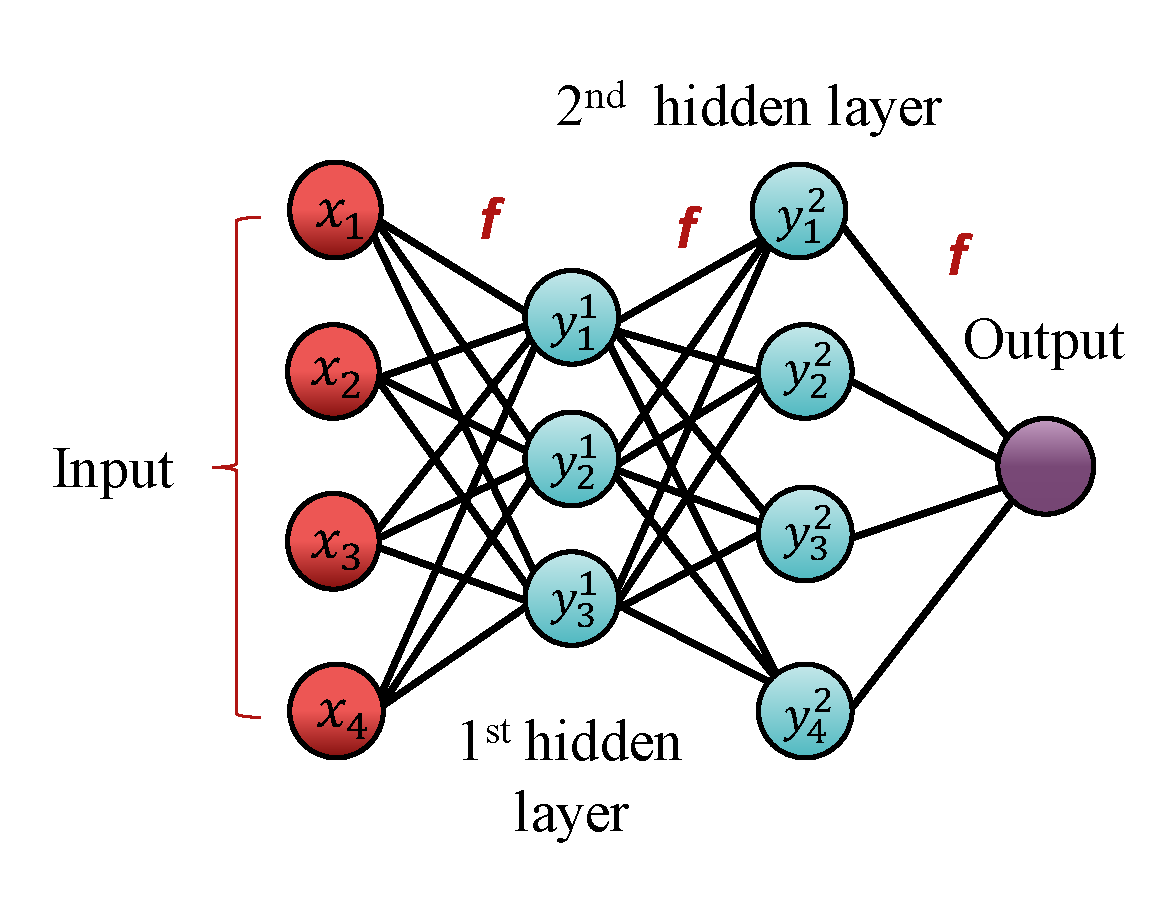
\includegraphics[width=.39\textwidth]{Figures/NN.pdf}
    \caption{Example scheme of a NN with two hidden layers.}
    \label{fig:NN}
\end{figure}

For the regression and classification tasks considered in this project the most natural choice is the FFNN, where each neuron has a non-linear activation function and is connected to all neurons in the subsequent layer. This type of NN is also called a fully-connected NN. All NN used in this project consist of at least three layers (input, hidden and output layer) and are also called multilayer perceptron (MLP) (see Fig.\ref{fig:NN}).

\subsubsection{Mathematical Model of MLP}
\label{subsubsec: MLP}

As it was mentioned, each neuron transforms an input signal from all neurons in the previous layer. Let us consider a node $i$ in the first hidden layer. The contribution of the input data points $x_j$ in $x_0, x_1, ..., x_{N_{in}}$ is regulated by the weights $w_{ij}$ and an additional bias $b_i$. The modified input can be written as:
\begin{equation}
\label{eq: 1}
    z_i = \sum_{j=0}^{N_{in}}w_{ij}x_j +b_i.
\end{equation}
Further, the way neuron fires as a response to this signal is defined by an activation function $f(\cdot)$ and forms an output sent to all neurons on the next layer:
\begin{equation}
    a_i = f\left(z_i\right)=\left(\sum_{j=0}^{N_{in}-1}w_{ij}x_j +b_i\right).
\end{equation}
Following the same logic, an output from a neuron $i$ in the layer $l$, $a_i^l$ can be written in terms of the outputs from the neurons in the layer $l-1$ as:
\begin{equation}
    a_i^l = f\left(z_i^l\right)=\left(\sum_{j=0}^{N_{l-1}-1}w_{ij}^la_j^{l-1} +b_i^l\right),
\end{equation}
or in the vector form:
\begin{equation}
    \textbf{a}^l=f(\textbf{W}^l\textbf{a}^{l-1}+\textbf{b}^l).
\end{equation}
This mathematical model introduces two matrices \textbf{W} and \textbf{b} (vector in the regression task) for each hidden layer. By analogy, an output layer transforms the signals from the last hidden layer $L$ and yields an an output $a_o$ by applying an output activation function $f_{out}(\cdot)$:
\begin{equation}
    \textbf{a}_o=f_{out}(\textbf{W}^{out}\textbf{a}^{L}+\textbf{b}^{out}).
\end{equation}
In overall, this yields $L+1$ (including output) matrices of parameters to be adjusted. The complete passage of the signal through the NN is called a forward pass (feed forward mechanism) and yields an output $\textbf{a}_o$, which should ideally reproduce the target values $y_0,y_1,...,y_{n_{out}}$ corresponding directly to the input vector. With an arbitrary choice of the weights and biases an output will unlikely be able to reproduce the target values, and therefore the weights and biases should be adjusted until the target value is reproduced within a certain accuracy.

\subsubsection{Choice of an Activation Function}
\label{subsubsec: activation function}

By analogy with the action potential on a membrane of a neuron, defining whether a neuron fires or not, an activation function controls an output from each node. This function should fulfill conditions of being non-constant, monotonically-increasing, bounded and continuous. In addition, the activation functions in the output layer should not be linear: in this case the output will be simply linear function of an input. This will make efficient learning of the NN practically impossible. In the simplest case a threshold $a$ is set and an output is set to zero if $z_i$ for a current neuron $i$ is below the threshold, thus switching "on" and "off". This type of activation function can be simply written with the Heaviside step function $H$ as:
\begin{equation}\label{eq:heaviside}
    f(z)=H(bz+c)=\begin{cases}
               0, \mbox{ }z<-c/b\\
               1, \mbox{ } z\geq -c/b\\
            \end{cases}.
\end{equation}
An efficient smooth alternative for the Heaviside function is the logistic Sigmoid function:
\begin{equation}
    f(z) = Sigmoid(z)=\frac{1}{1+e^{-z}}.
\end{equation}
This function constrains an output from a neuron, compressing it to a value from 0 to 1. An output of inactive neuron is set to 0 (one-sided function) and, as compared to the Heaviside, this activation function has defined derivatives for the whole range of $z$ values. Similar alternative to the step function is the hyperbolic tangent:
\begin{equation}
    f(z)=tanh(z)=\frac{e^z-e^{-z}}{e^z+e^{-z}}.
\end{equation}
This function was found to be particularly effective for training MLP and will be tested alongside Sigmoid function in this project. 

In order to avoid identity activation function $f(z)=z$, the so-called rectifier (ReLU, rectifying linear unit) is introduced:
\begin{equation}
    f(z)=\begin{cases}
               0, \mbox{ }z<0\\
               z, \mbox{ } z\geq 0\\
            \end{cases}.
\end{equation}
Simplicity of this function yields potentially efficient computation and smaller CPU times. By analogy with the Sigmoid, it is biologically plausible due to setting outputs of inactive neurons to 0. In addition, it is invariant to scaling and mitigates problem of vanishing gradients in the training procedure. However, it shares the same problem with the step function, by being non-differentiable at zero. In addition, it is unbound for high $z$ values. Another issue, so-called dying ReLU problem, is related to some neurons being hut down(deactivated) so that the signal does not pass through it while training and updating the weights and biases. This can, however, be resolved by allowing a certain linear dependence of an output on the input with leaky ReLU:
\begin{equation}
    f(z)=\begin{cases}
               az, \mbox{ }z<0\\
               z, \mbox{ } z\geq 0\\
            \end{cases},
\end{equation}
where $a$ is a small value, \textit{e.g.} 0.001. In this project the latter four activation functions will be tested for hidden layers.

Finally, the activation function of the output layer yields directly a result to be compared with the target values. For the regression problem adjustment of the weights and biases for all hidden layers and the output layer should be sufficient to be able to reproduce the target. Therefore, a simple identity function $f(z)=z$ is proposed for the output layer. On the contrary, for the classification problem one would be interested in probabilities for a given input point to be attributed to a certain class. As all probabilities should add up to 1, the Softmax function was used for the activation of an output layer (see Eq.\ref{eq:softmax}). With this choice of output activation functions architecture of a NN can be further modified by combining different activation functions for hidden layers to improve an overall performance.

\subsubsection{Back Propagation Mechanism}
\label{subsubsec: back propagation}

As it was already mentioned, the weights and biases in each hidden layer and an output layer should be adjusted for the NN to be able to reproduce its target. In order to do that, the cost function $C(\cdot)$ reflecting directly proximity of the produced result to the target is introduced. The aim now is to find optimal parameters \textbf{W} and \textbf{b} minimizing the cost function. In the most general case, $C(\cdot)$ is a function of an output from the last layer $O$ (output layer), $a_i^O$ and target values $t_i$. We are now in interested in how the cost function changes with respect to the biases and weights of the output layer $\textbf{W}^O$ and $\textbf{b}^O$. According to the chain rule:
\begin{equation}
    \frac{\partial C(a_j^O, t_j)}{\partial w_{ij}^O}=\frac{C(a_j^O, t_j)}{\partial a_{j}^O}\frac{\partial a_{j}^O}{\partial z_{j}^O}\frac{\partial z_{j}^O}{\partial w_{ij}^O}.
\end{equation}
Let us consider all terms in this equation. The first one is firectly defined by the choice of a specific cost function and will be considered later. The second term is defined by the derivative of an output activation function as:
\begin{equation}
    \frac{\partial a_{j}^O}{\partial z_{j}^O} = f^{\prime}(z_{j}^O).
\end{equation}
The last term yields simply (see Eq.\ref{eq: 1}):
\begin{equation}
    \frac{\partial z_{j}^O}{\partial w_{ij}^O}=a^L_i,
\end{equation}
where $L$ denotes the last hidden layer. Combining all together we can express the change of the cost function with respect to $w_{ij}^O$ in terms of an output error $\delta_{j}^O$:
\begin{equation}
    \frac{\partial C(a_i^O, t_i}{\partial w_{ij}^O}=f^{\prime}(z_{j}^O)\frac{\partial C(a_j^O, t_i)}{\partial a_{j}^O}a^L_i= \delta_j^Oa^L_i
\end{equation}
The error $\delta_j^O=f^{\prime}(z_{j}^O)\frac{C(a_j^O, t_i)}{\partial a_{j}^O}$ for an output layer reflects directly how fast the cost function changes with an output activation. It can be also obtained that:
\begin{equation}
    \frac{\partial C(a_j^O, t_i)}{\partial b_{j}^O}=\delta_j^O.
\end{equation}
Replacing the output layer $O$ with a general layer $l$ one can obtain the relation of an error in $l$-th layer to the error in the next $l+1$-th layer:
\begin{equation}
\label{eq: 2}
    \delta_j^l=\frac{\partial C}{\partial z_{j}^l}=\sum_k \frac{\partial C}{\partial z_{k}^{l+1}}\frac{\partial z_{k}^{l+1}}{\partial z_{j}^{l}}=\sum \delta_k^{l+1}\frac{\partial z_{k}^{l+1}}{\partial z_{j}^{l}}.
\end{equation}

Taking into account the relations between $z_{k}^{l+1}, a_{k}^{l}$ and $z_{k}^{l}$, namely  $z_{k}^{l+1}=\sum_{i=0}^{N_l}w_{ik}^{l+1}a_i^l+b^{l+1}_k$ and $a_{k}^{l}=f(z_{k}^{l})$, one can rewrite Eq.\ref{eq: 2} in the following form:
\begin{equation}
    \delta_j^l=\sum_k \delta_k^{l+1} w_{jk}^{l+1}f^{\prime}(z_j^l).
\end{equation}
Thus, the error in a layer $l$ can be propagated back, towards the first hidden layer. This is the core equation of the back propagation mechanism, allowing to update biases and weights based on the feedback from the cost function. The cost function is minimized through series of such updates. The gradients of the cost function $\frac{\partial C}{\partial w_{ij}^l}$ and $\frac{\partial C}{\partial b_{j}^l}$ containing the error for the layer $l$ are used to update the weights and biases for each $l=O, L, L-1, ...2$ as:
\begin{equation}
    w^l_{jk}\rightarrow w_{jk}^l-\eta\delta_j^la_k^{l-1},
    b_j^l\rightarrow b_j^l-\eta\delta_j^l,
\end{equation}
where $\eta$ is the learning rate. Therefore,  Gradient Desencent can be seen as the the core mechanism of learning (updating of all parameters) in the NN. Let us assume that the data set is split into $M$
minibatches, then the full forward pass of a current minibatch followed by the back propagation is called an iteration. The full training period for all $M$ minibatches is called an epoch in the context of the NN. Depending on the choice of a minibatch size and, thus, number of iterations, learning rate, initial choice of weights and biases and number of epochs, the accuracy or the resulting scores can vary significantly. By tuning these parameters and modifying the architecture of the NN one could approximate a desired target with desired accuracy. This is indeed in accordance with the Universal approximation theorem, stating that a FFNN with one hidden layer and a fine number of neurons in it can approximate a continuous multidimensional function with an arbitrary chosen accuracy, given an activation function fulfilling all necessary requirements. 

All equations listed above are written in their general form and should be specified for a particular cost, hidden layer and output activation functions. For the regression problem, the natural choice of cost function is a sum of squared residuals, by analogy with that in the Project 1:
\begin{equation}
    C(a_j^O, t_j)=\frac{1}{2}\sum_{j=0}^{N_O}(a_j^O-t_j)^2.
\end{equation}
 This form of the cost function yields:
 \begin{equation}
     \frac{C(a_j^O, t_j)}{\partial a_{j}^O}=(a_{j}^O-t_j).
 \end{equation}
 An output activation function, as discussed above, is a simple identity function $f(z)=z$, yielding $f^{\prime}(z)=1$. Collecting all these expression, the error in the output layer can be written explicitly as:
 \begin{equation}
     \delta_j^O = a_{j}^O-t_j.
 \end{equation}
 
 For the case of the multiclass classification problem the typical choice of the cross-entropy, or negative log likelihood function, expressed as:
 \begin{equation}
     C(a_j^O, t_j)=-\sum_{j=0}^{N_O}\left(t_j\log{a_j^O}+(1-t_j)\log{a_j^O}\right).
 \end{equation}
 Writing its derivative with respect to the $a_j^O$ values provides us with:
  \begin{equation}
     \frac{C(a_j^O, t_j)}{\partial a_{j}^O}=\frac{t_j}{a_j^O}-\frac{1-t_j}{1-a_j^O}=\frac{t_1-a_j^O}{a_j^O(1-a_j^O)}.
 \end{equation}
 The activation function choice, previously discussed, is the Softmax function, yielding the derivative:
 \begin{equation}
     f^{\prime}(z_j^O)=f(z_j^O)(1-f(z_j^O))= a_j^O(1-a_j^O).
 \end{equation}
 Both equations end up in the output error given by:
 \begin{equation}
     \delta_j^O=a_j^O(1-a_j^O)\frac{t_1-a_j^O}{a_j^O(1-a_j^O)}=a_{j}^O-t_j,
 \end{equation}
 which is exactly the same result as in case of the regression problem. Hence, the same equations will be used to perform both regression and classification types of analysis. The only expression left is the derivative of an activation layer $l$ used for the propagation of the error in the backward direction. Since different activation functions can be assigned to different hidden layers, all options for the activation functions and their derivatives is included in the code for this project.
 %----------------------------------------------------------
 
 \subsection{Metrics}\label{subsec: metrics}
 
 In order to asses performance of the model (in our case, a NN) one has to introduce statistical characteristics relating the target values with an obtained prediction. The $R^2$ and MSE scores are the natural choice to estimate deviation of the predictions from the actual value in case of a regression problem. They are used in this Project for the Franke's function-based dataset. Both definitions are are described and discussed in more detail in the previous project \cite{proj1, proj1_2}.
 
In contrast to predicting continuous values, an assessment of how well a machine performs by guessing a class (discrete value) was carried out in terms of the accuracy. This metric is simply defined as the number of correctly guessed targets $t_i$ divided by the total number of targets, \textit{i.e.} \cite{Morten}:
 \begin{equation}
     \mathrm{Accuracy} = \frac{\sum_{i=1}^{n} I(t_i = y_i)}{n}.
 \end{equation}
 Here the $I$ is the indicator function, giving 1 if $t_i = y_i$ and $0$ otherwise. The $t_i$ represents the target and $y_i$ represents the outputs of our neural network, and $n$ is the total number of targets.
 
\section{Studied models}
\label{sec: Studied models} 

\subsection{Franke Function}\label{subsec: franke function}

All methods described in the previous sections were tested on the dataset acquired with the Franke's function with added noise, by analogy with Project 1. We hereby refer to Project 1 for more information about the form of the Franke's function \cite{proj1, proj1_2}. This dataset provides us with a good test example where various methods performing regression can be compared on the same footing. The noise added is normally distributed $\sim\mathcal{N}(0,1)$ and modulated by an amplitude $\alpha=0.001$. Such a small noise reduces probability of the standard gradient descent procedure to be stuck in numerous potential  local minima of the cost function and makes it, presumably, less dependent on the initial choice of the regression parameter $\beta$.  For the present project, the Franke's function is defined on the regular grid $x\in[0,1]$ and $y\in[0,1]$ with $N\timesN=30\times 30=900$ data points in overall.

The first step of the analysis is again scaling of the dataset as discussed in \cite{proj1, proj1_2}. Since the GD and SGD are involved, scaling of the data might become crucial for the convergence of the procedure. The study in Project 1 was found to be less sensitive to weather the dataset is scaled or not, but in the presented case might result in reduction of the number of epochs used (for the same learning rate) and, therefore, decrease the CPU run time. The second step implies creation of the design matrix $X$ for a chosen polynomial degree \cite{proj1, proj1_2}. From now on we limit ourselves to the polynomial degree 5, which reproduces the main features of the function without slowing down the computational procedure due to the particularly large dimensions of the design matrix. This matrix, together with the values of the Franke's function presents the main input for the GD, SGD and the FFNN, which will be first trained on the training subset of the design matrix and the Franke's function and subsequently applied to the test set of data. 

\subsection{MNIST Data}\label{subsec: mnist data}

The Neural Network developed in this project was also tested on the MNIST hand-written numbers database \cite{MNIST}. Here, a picture of a hand written digit was input to the neural network, with a goal of \textquotedblleft reading\textquotedblright the value. Where the Franke's function was a continuous function and we were interested in predicting its value for a data point in the grid, the MNIST database provides an opportunity to work with the classification problem where we are interested in an exact discrete output value between $0-9$.
\begin{figure}[h]
    \centering
    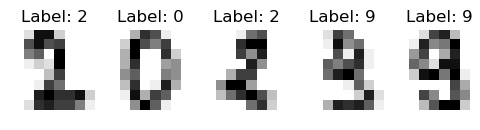
\includegraphics[width=.49\textwidth]{Figures/MNIST_illustrated.png}
    \caption{Examples of hand written numbers from the MNIST database used for this project. The label shows what digit it is supposed to be.}
    \label{fig:MNIST_illustrations}
\end{figure}

From the MNIST database we collect gray-scale images with the size of $8x8$ pixels (see Fig. \ref{fig:MNIST_illustrations}). For simplicity, the number of pixels are reduced from the original values of $28x28$. Since each input picture is a 2D matrix, it was \textquotedblleft unraveled\textquotedblright to a vector with $64$ inputs. Each vector element is then a number between $0$ and $1$, representing the gray-scale intensity, and additionally labelled by this number. These labels will be the target values we will be aiming at reproducing.

As for a typical multiclass classification problem, it is convenient to convert the labels attributed to each image into the so-called \textit{one-hot} vectors. 
Therefore, the NN will output a one-hot vector by using the Softax activation function in the outpuut layer from an input image and will be compared with the target one-hot vector in the training procedure. The cost-function as well as the output error of the NN model is calculated from a relation between the input and the output one-hot vector in terms of the cross-entropy. A one-hot vector has the size of the number of classes, where each value corresponds to the probability that the input image represents a certain class. For example, the input one-hot vector for an image of the written digit "2" will  look like 
\begin{equation}
y=2 \rightarrow \hat{y}_{input} = \{0,0,1,0,0,0,0,0,0,0\}
\end{equation}
i.e. the probability that this image represents the number $2$ is $100\%$. The output one-hot vector might for example look like 
\begin{equation}
y=2 \rightarrow \hat{y}_{output} = \{0,0,0.8,0,0,0,0.5,0,0.15,0\}    
\end{equation}
saying it is a $80\%$ chance the image represents the number $2$, $15\%$ chance it is an $8$ and a $5\%$ chance it is a $6$.

After the training procedure is accomplished, there is no need to convert the dataset one wants to make a prediction for into a one-hot representation. Instead, prediction of a label is made by picking an index of an element with maximum probability in an output one-hot vector. An obvious advantage of such representation of labels and images is that rescaling of the input data is no longer crucial for the convergence of the SGD.

%-----------------------------------------------------------
\section{Code} \label{sec: Code}

The study of the regression and classification problems for the Franke's and MNIST data combined with an application of the stochastic gradient descent was performed with the set of Python3-based codes which can be accessed from Appendix.A(\ref{Appendix:A}). The major improvement of the code, as compared to the code for the Project 1 \cite{proj1,proj1_2} is introduction of the classes, used for more efficient structuring of the computational procedure for all tasks. Interpreting a neural network as an object of a neural network class is a natural and efficient choice for the work with various types of networks with adjustable parameters and architectures. In addition, the functions used for performing direct work with and preprocessing of input data, resampling methods and regression methods were combined into three interconnecting classes. 

\begin{figure}[h]
    \centering
    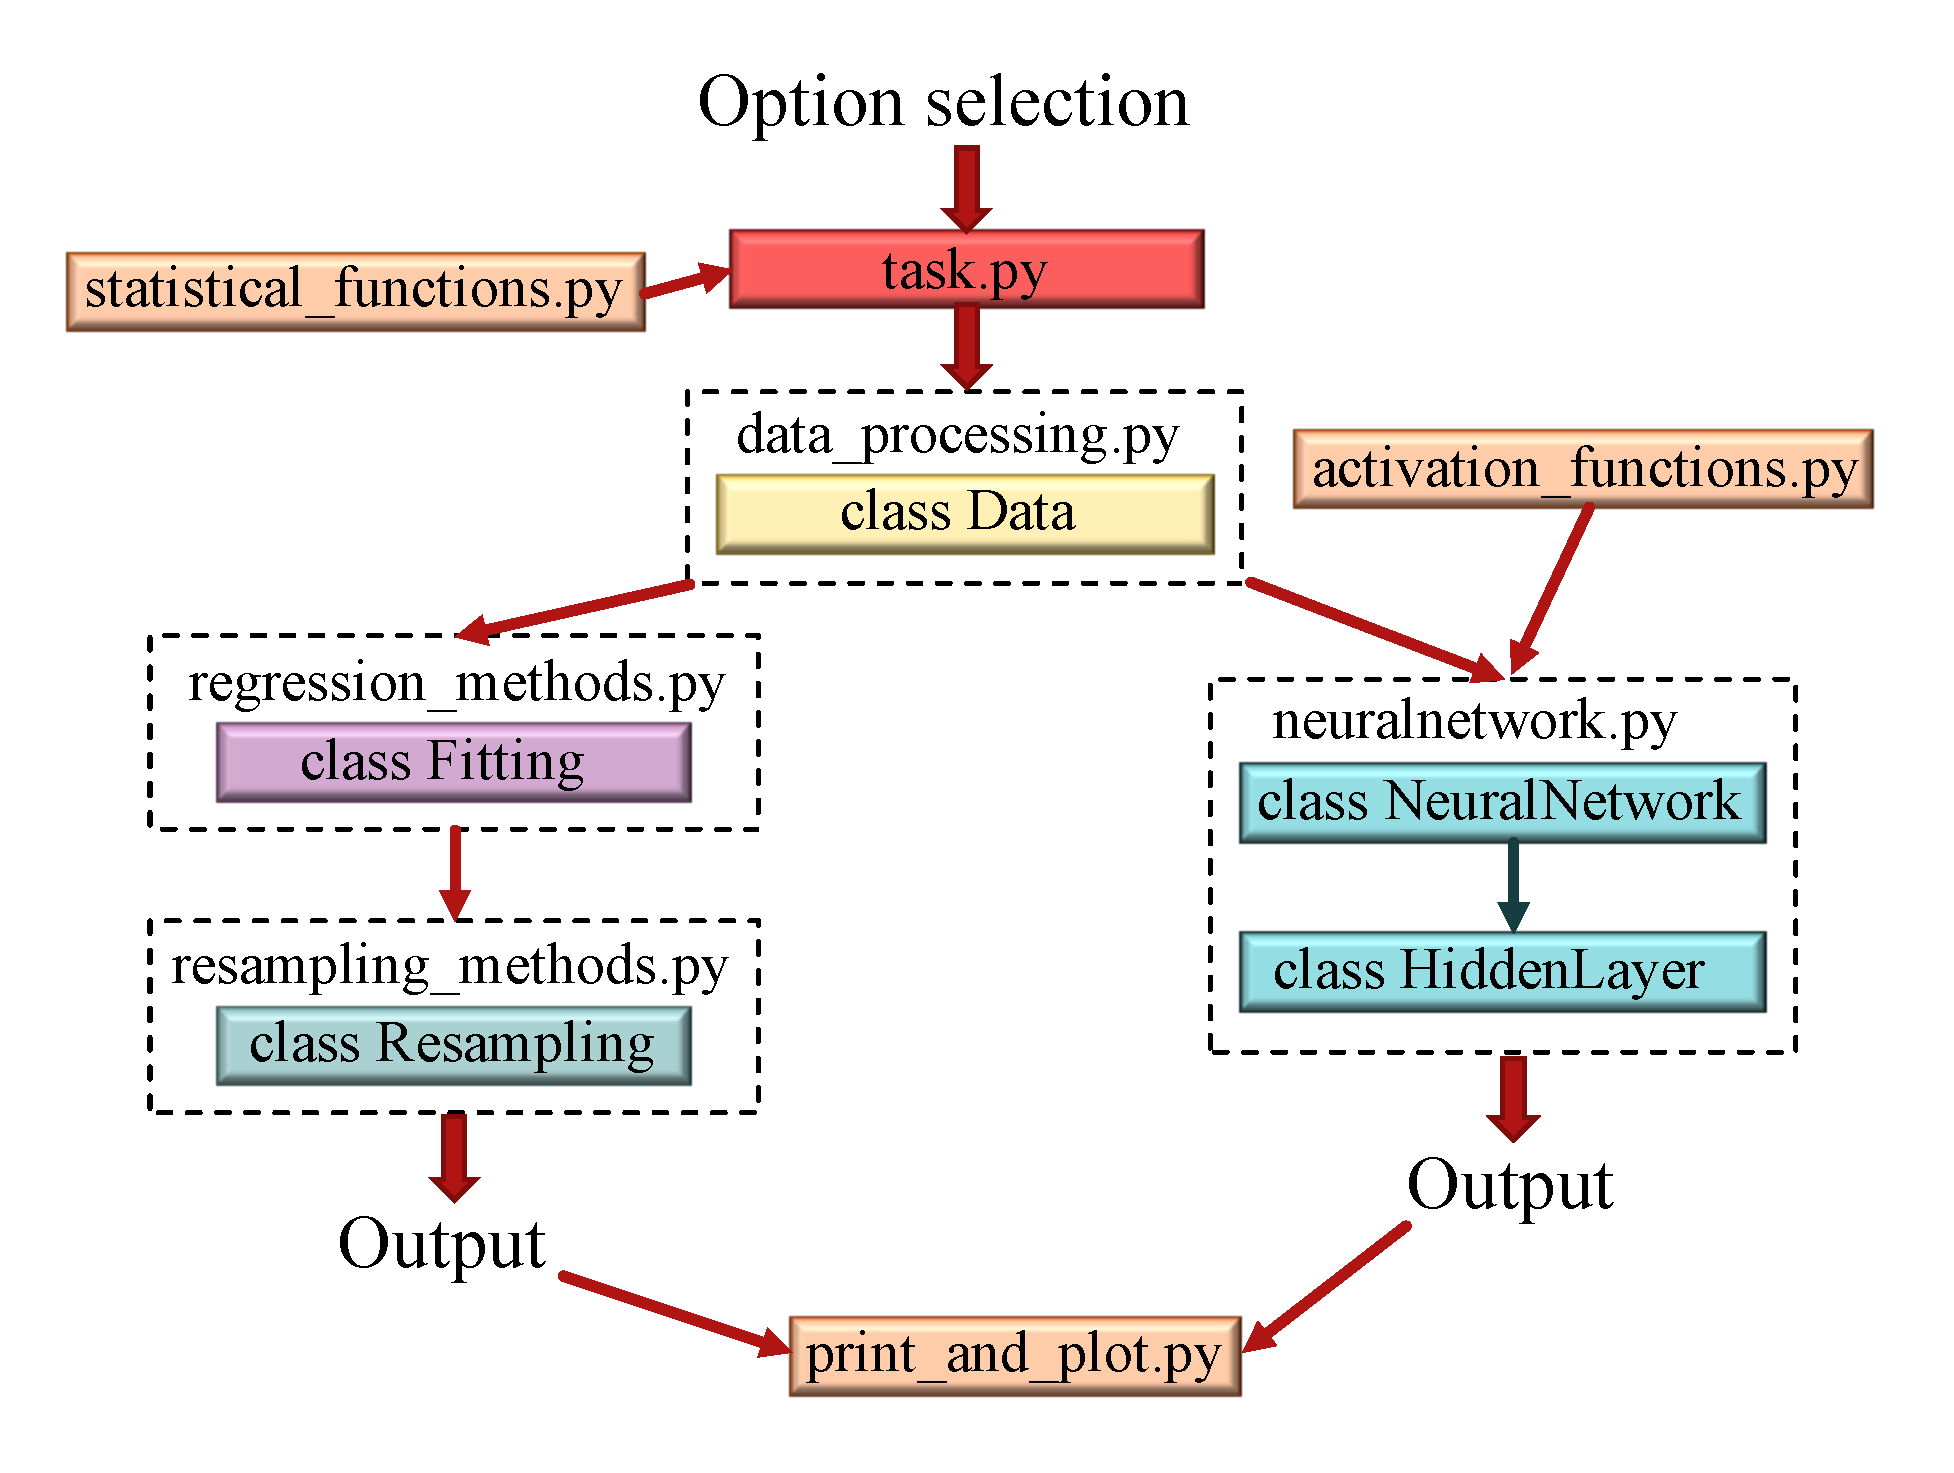
\includegraphics[width=.49\textwidth]{Figures/code.pdf}
    \caption{Principal scheme of the code used in the project.}
    \label{fig:code}
\end{figure}

The principal scheme of the components of the code is shown in Fig.\ref{fig:code}. In order to collect results for different cases \textit{task\_a.py}, \textit{task\_b.py}, \textit{task\_c.py}, \textit{task\_d.py}, and \textit{task\_e.py} files were run. In each file several user-defined study options are available, \textit{e.g.} study of the test and training scores as functions of the learning rate, number of epochs, grid search, \textit{etc.} Resulting scores are written to files used further for graphical interpretation of the results, presented in the following section.


For the first task an object \textit{franke\_function} of the class \textit{Data} (\textit{data\_processing.py} is created and prepared for the implementation of regression with the attributed class methods, \text{e.g.} by setting a grid and the Franke's function (\textit{set\_grid\_franke\_function(...)}, \textit{set\_franke\_function()}), adding noise (\textit{add\_noise()}) and scaling with the Scikit-Learn functionality \textit{sklearn.preprocessing.StandardScaler} \cite{skl}. Further, an additional object \textit{model} of the class \textit{Resampling} (\textit{resampling\_methods.py}) is created on the base of an existing \textit{Data} object. For the presented study we keep two possible options for the analysis of the scores, namely k-fold cross-validation and no-resampling method exploiting \textit{sklearn.model\_selection.train\_test\_split} functionality from Scikit-Learn \cite{skl}. For the project, if k-fold cross-validation is not chosen, the input data are split into the test and training subsets with this functionality, implemented as a class \textit{Data} method, in proportion  80\% training/ 20\% test data. This was shown to be a suitable ratio for effective training in Project 1 \cite{proj1}. For the k-fold cross-validation 5 folds case was used based on its good performance for the score assessment for the Franke's data in the first Project \cite{proj1,proj1_2} and relatively small CPU run time as compared to the higher number of folds. Splitting of data into minibatches is performed with the \textit{split\_minibatch(...)} routine of \textit{Data} class. Since this method is used for both the k-fold cross-validation (all data into minibatches) and SGD (training data into minibatches), a user can choose which dataset will be divided into minibatches or divide both of them. 

Both resampling options perform fitting of the data (class \textit{Fitting}, \textit{regression\_methods.py} object) by either OLS (\textit{OLS()}) or ridge (\textit{ridge(...)}) with the standard matrix SVD-based matrix inversion \textit{numpy.linalg.pinv} \cite{numpy}. The new cost function minimization options include SGD (\textit{SGD()}) for the cases with and without penalty ($\lambda>0$) included, standard GD and the Scikit-Learn functionality \textit{sklearn.linear\_model.SGDRegressor} \cite{skl}. The mechanism of the SGD tested in the first task is further implemented in the neural network.


As it was already mentioned, the neural network in the second task is set and interpreted as an object of the \textit{NeuralNetwork(...)} class in \textit{neuralnetwork.py}. Setting of the network is flexible and implies different architecture types with variable number of hidden layers, neurons in each layer, activation functions for the hidden and output layers. In order to facilitate setting of the new hidden layers, and additional class \textit{HiddenLayer(...)} was created, collecting all inputs and outputs from each neuron in a given hidden layer. The principal components of the NN are listed below:

\begin{lstlisting}[language=Python, caption={Structure of the NeuralNetwork and HiddenLayer classes}]
import numpy as np
from activation_functions import *

class NeuralNetwork:
    def __init__(NN parameters):
        ''' FFNN class, setting of all SGD parameters, 
        penalty hidden and output weights  '''
        
    def create_output_biases_and_weights(self):
        '''Setting of normally distributed 
        output weights and constant output bias'''
        
    def feed_forward(self):
        '''Forward pass for a selected 
        minibatch'''
        
    def backpropagation(self):
        ''' Back propagation mechanism for a 
        given minibatch, updating weights and biases'''
        
    def train(self):
        ''' Training for a selected number of 
        epochs for all minibatches with 
        random selection of data into 
        minibatches'''
        
    def predict(self, X):
        ''' Prediction of an output value for 
        the regression problem'''
        
    def predict_class(self, X):
        '''Prediction of an output value for 
        the classification problem'''


class HiddenLayer:
    def __init__(layer parameters):
        '''Hidden layer class containing 
        information on inputs and outputs for 
        each node in a givel layer'''
        
    def hidd_act_function(self, x):
        '''Returns a selected activation 
        function for a given hidden 
        layer'''
        
    def hidd_act_function_deriv(self, x):
        '''Returns a derivative of a selected 
        activation function for a given hidden 
        layer'''
        
    def create_biases_and_weights(self):
        '''Setting of normally distributed 
        weights and a constant bias for a 
        hidden layer'''
\end{lstlisting}

Training procedure combines passage of each randomly selected (without replacement) minibatch in the forward direction through the whole NN and its back propagation looped over a selected number of minibatches and epochs. Such setting of the NN provides us with a considerable freedom to adjust the architecture to achieve the best scores. This will be shown in the next section for the regression problem on the Franke's data. In addition, the NN can be easily adapted for the classification problem by switching to the different (cross-entropy) cost function, output activation function (Softmax) and number of output categories. For both cases, the regression and classification, performance of this NN is compared to the in-built Scikit-Learn functionalities, namely \textit{sklearn.neural\_network.MLPRegressor} and \textit{sklearn.neural\_network.MLPClassifier} \cite{skl} with the same settings of the layer initialization, SGD parameters and regularization parameter (SKL NN). In addition, we compare performance of all above-mentioned NN \textit{vs.} the Keras NN, running on top of the machine learning platform TensorFlow \cite{keras}. In overall, Keras provides us with even more freedom in designing a NN , by \textit{e.g.} choosing different activation functions and for different hidden layers and their initialization. In this sense, the Scikit-Learn is more limited, but still an effective tool for the proposed analyses. For this project we aim to compare performance of all three types of NN with the same settings without exploring the whole computational power of Keras-based NN. For the classification task, all studies of the SKL and Keras NN is kept in the \textit{project2.ipynb} Jupiter notebook, exploiting \textit{keras\_NN.py} functionality for the faster representation of the results.  

Finally, for the last task, including classification of the MNIST data, the logistic regression based on the SGD and GD was written and included as a routine of the \textit{Fitting} class. Performance of this logistic regression function was also compared with the implemented Scikit-Learn functionality \textit{sklearn.linear\_model.LogisticRegression}, also included, as an option, in the logistic regression routine.


All classes and task files share access to the functions from \textit{statistical\_functions.py}, returning desired metrics. The \textit{NeuralNetwork} class has an additional access to all implemented activation functions and their derivatives. The obtained results, written to files, were plotted by running a chosen option from the \textit{print\_and\_plot.py} file and are presented in the next section.

%-----------------------------------------------------------------
\hspace{1cm}
\section{Results} 
\label{sec: Results}

%---------------------------Task a----------------------------
\subsection{Testing stochastic gradient descent}
\label{subsec: Task 1}
As a first step, the Franke's  function analysis from Project 1 \cite{proj1, proj1_2} was performed again,but using stochastic gradient descent (SGD) with both the ordinary least square regression (OLS) and ridge regression instead of the matrix inversion. For all the results for the Franke's function analysis we used 5-fold cross-validation resampling method to increase stability and reliability of the results.

The resulting $R^{2}$ scores and MSEs for the training and test datasets as functions of the learning rate $\eta$ for OLS is shown in Fig.\ref{fig: R2_OLS_eta} and Fig.\ref{fig: MSE_OLS_eta} respectively. The results show a very slight difference between the training and test data, where the $R^{2}$ is slightly bigger for the training set, whereas the MSE is lower for the training set, as might be expected for this choice of the design matrix. For a selected range of the learning rates, both the training and test $R^{2}$ seem to increase monotonously (MSE decreases monotonously) for a chosen number of epochs and minibatch size $N_{\mathrm{epochs}}=1000$ and minibatch size $M=5$ (will be denoted by $M$ from now own).

\begin{figure}[h]
    \centering
    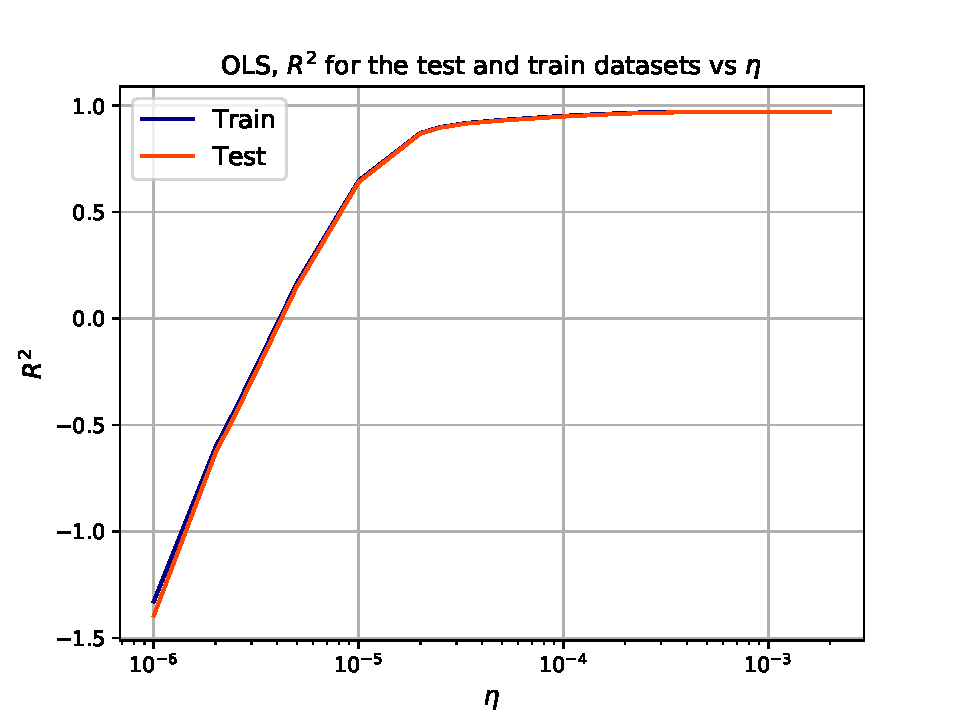
\includegraphics[width=.49\textwidth]{Figures/OLS_R2_eta.pdf}
    \caption{$R^2$ scores for the test and training datasets obtained with SGD and 5-fold cross-validation with $N_{\mathrm{epochs}}=1000$ and $M=5$ for different learning rates. OLS ($\lambda=0.0)$ case.}
    \label{fig: R2_OLS_eta}
\end{figure}

\begin{figure}[h]
    \centering
    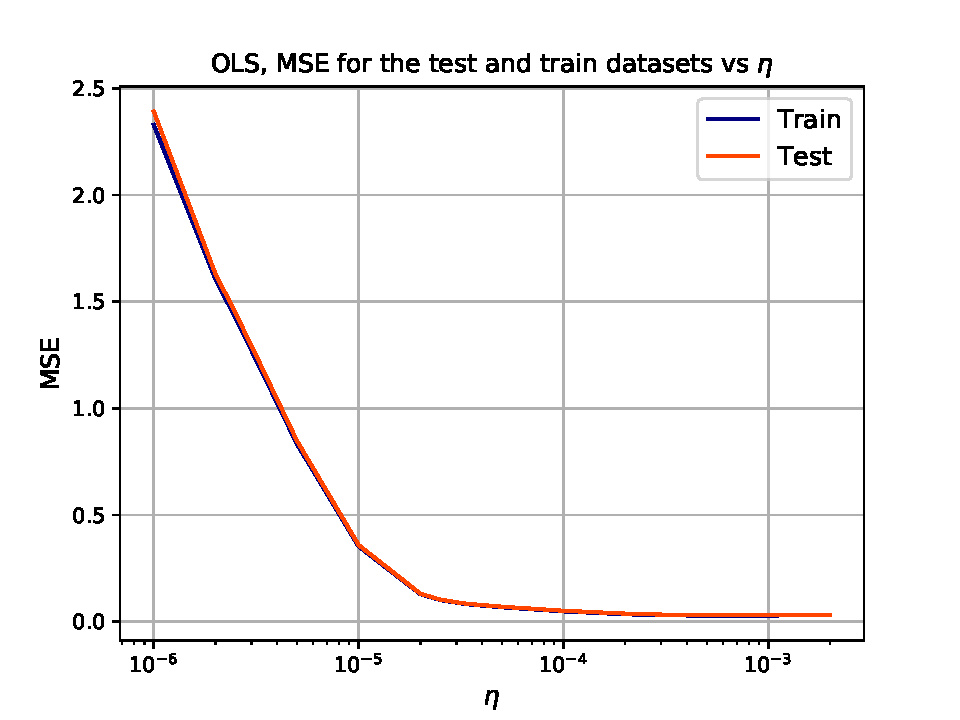
\includegraphics[width=.49\textwidth]{Figures/OLS_MSE_eta.pdf}
    \caption{MSE for the test and training datasets obtained with SGD and 5-fold cross-validation with $N_{\mathrm{epochs}}=1000$ and $M=5$ for different learning rates. OLS ($\lambda=0.0)$ case.}
    \label{fig: MSE_OLS_eta}
\end{figure}

The OLS $R^{2}$ test and training scores and MSEs as functions of a minibatch size are presented in Fig.\ref{fig: R2_OLS_minibatch} and \ref{fig: MSE_OLS_minibatch}. It seems to show that the optimal size of the minibatch is around $M\approx5-10$. For the further increase of $M$ a fast worsening of the results is observed. 

\begin{figure}[h]
    \centering
    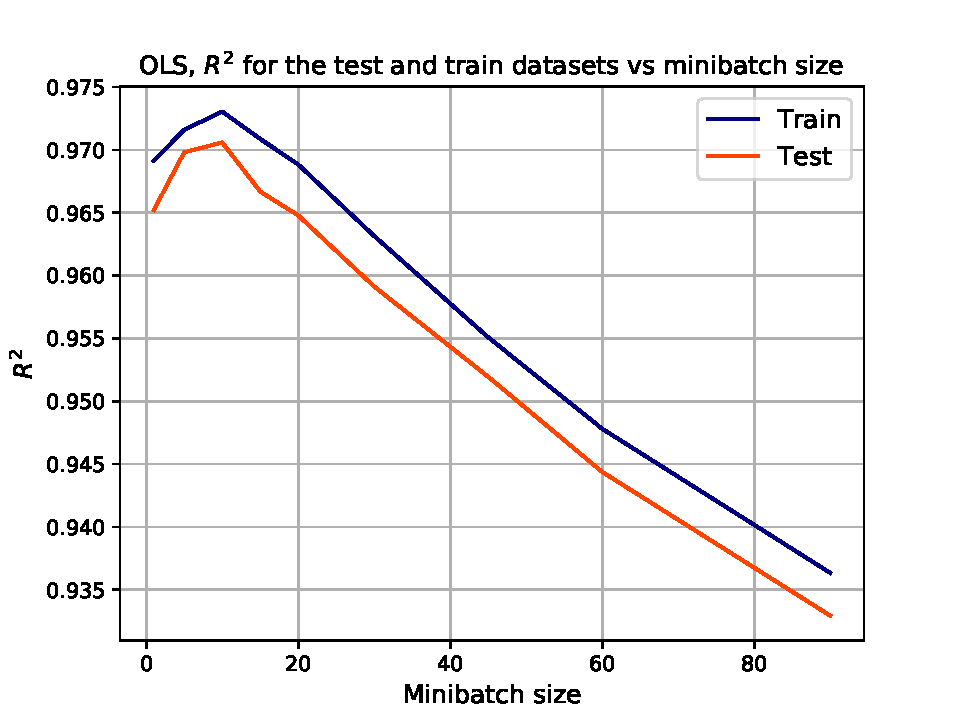
\includegraphics[width=.49\textwidth]{Figures/OLS_R2_minibatch.pdf}
    \caption{$R^2$ scores for the test and training datasets obtained with SGD and 5-fold cross-validation with $N_{\mathrm{epochs}}=1000$ and $\eta=0.001$ for different sizes of minibatches. OLS ($\lambda=0.0)$ case.}
    \label{fig: R2_OLS_minibatch}
\end{figure}

\begin{figure}[h]
    \centering
    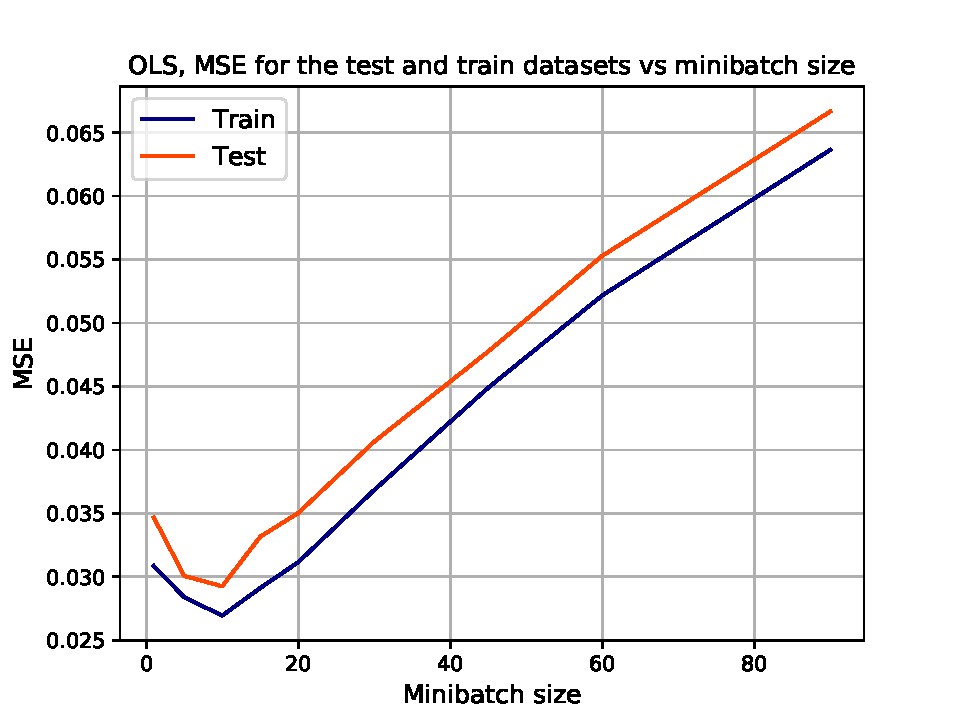
\includegraphics[width=.49\textwidth]{Figures/OLS_MSE_minibatch.pdf}
    \caption{MSE for the test and training datasets obtained with SGD and 5-fold cross-validation with $N_{\mathrm{epochs}}=1000$ and $\eta=0.001$ for different sizes of minibatches. OLS ($\lambda=0.0)$ case.}
    \label{fig: MSE_OLS_minibatch}
\end{figure}

To also study the effect of the number of epochs, the $R^{2}$ scores for the test and training sets and MSE for OLS were also studied as functions of epochs. These results are shown in Fig.\ref{fig: R2_OLS_epochs} and Fig.\ref{fig: MSE_OLS_epochs} respectively. The optimal number of epochs seem to be $\approx 1000$, after which it seems to be essentially constant with increasing epochs. For the chosen learning rate $\eta=0.001$ and the minibatch size $M=5$ further increasing of $N_{\mathrm{epochs}}$ does not seen to lead to any significant improvements, meaning that the SGD was able to converge properly.

\begin{figure}[h]
    \centering
    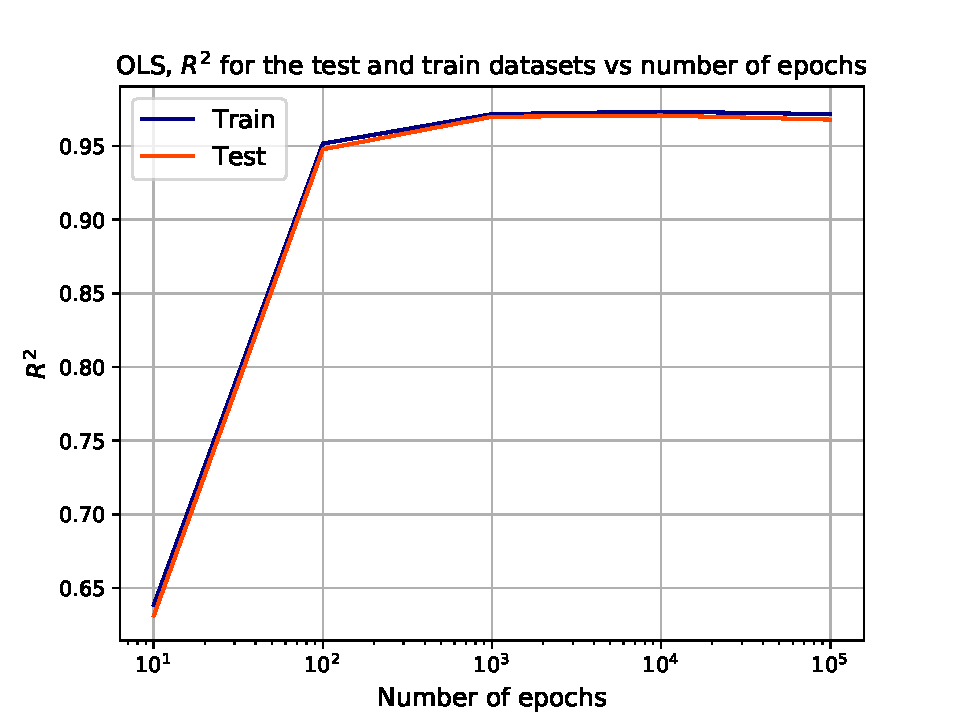
\includegraphics[width=.49\textwidth]{Figures/OLS_R2_epochs.pdf}
    \caption{$R^2$ scores for the test and training datasets obtained with SGD and 5-fold cross-validation with $M=5$ and $\eta=0.001$ for different numbers of epochs. OLS ($\lambda=0.0)$ case.}
    \label{fig: R2_OLS_epochs}
\end{figure}

\begin{figure}[h]
    \centering
    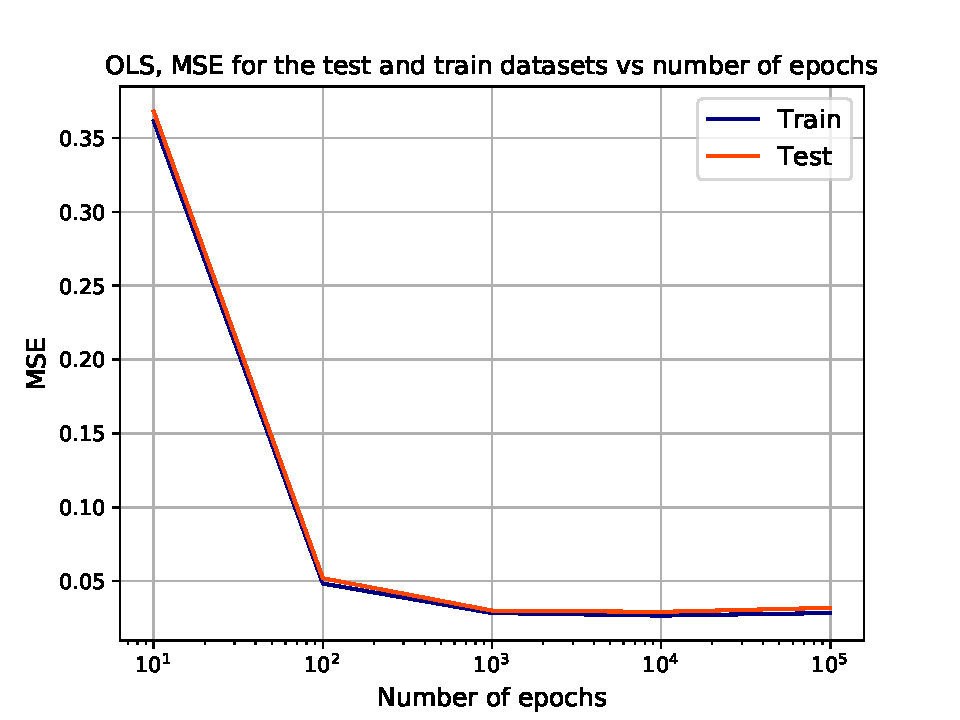
\includegraphics[width=.49\textwidth]{Figures/OLS_MSE_epochs.pdf}
    \caption{MSE for the test and training datasets obtained with SGD and 5-fold cross-validation with $M=5$ and $\eta=0.001$ for different numbers of epochs. OLS ($\lambda=0.0)$ case.}
    \label{fig: MSE_OLS_epochs}
\end{figure}

When it comes to the ridge regression results with SGD, a grid search was performed to find the optimal $\lambda$ and $\eta$. The $R^{2}$ score and MSE for the test and training datasets  for zero and non-zero regularization parameters are presented in Figures \ref{fig: Ridge_grid_R2_coarse} and \ref{fig: Ridge_grid_MSE_coarse} respectively. These results use a coarse learning rate grid with the step of one order of magnitude. We also present results with a fine learning rate grid where Fig.\ref{fig: Ridge_grid_R2_fine} and Fig.\ref{fig: Ridge_grid_MSE_fine} show the resulting $R^{2}$ scores and MSEs respectively for a selected set of learning rates, thus zooming the area of the best scores presented in the previous figures. These fine scale results are used for a better representation of the area with the highest $R^{2}$ scores (and lowest MSE). The white spots encountered in the grid denote the cases where results can not be obtained due to a computational overflow.

In addition, the study of the $R^2$ scores and MSE for the case of non-zero regularization parameter $\lambda=0.1,0.01,0.001$ was also performed. But due to the similar trends they are not included into the main discussion part and presented in Appendix C \ref{Appendix:C}. 

\begin{figure}[h]
    \centering
    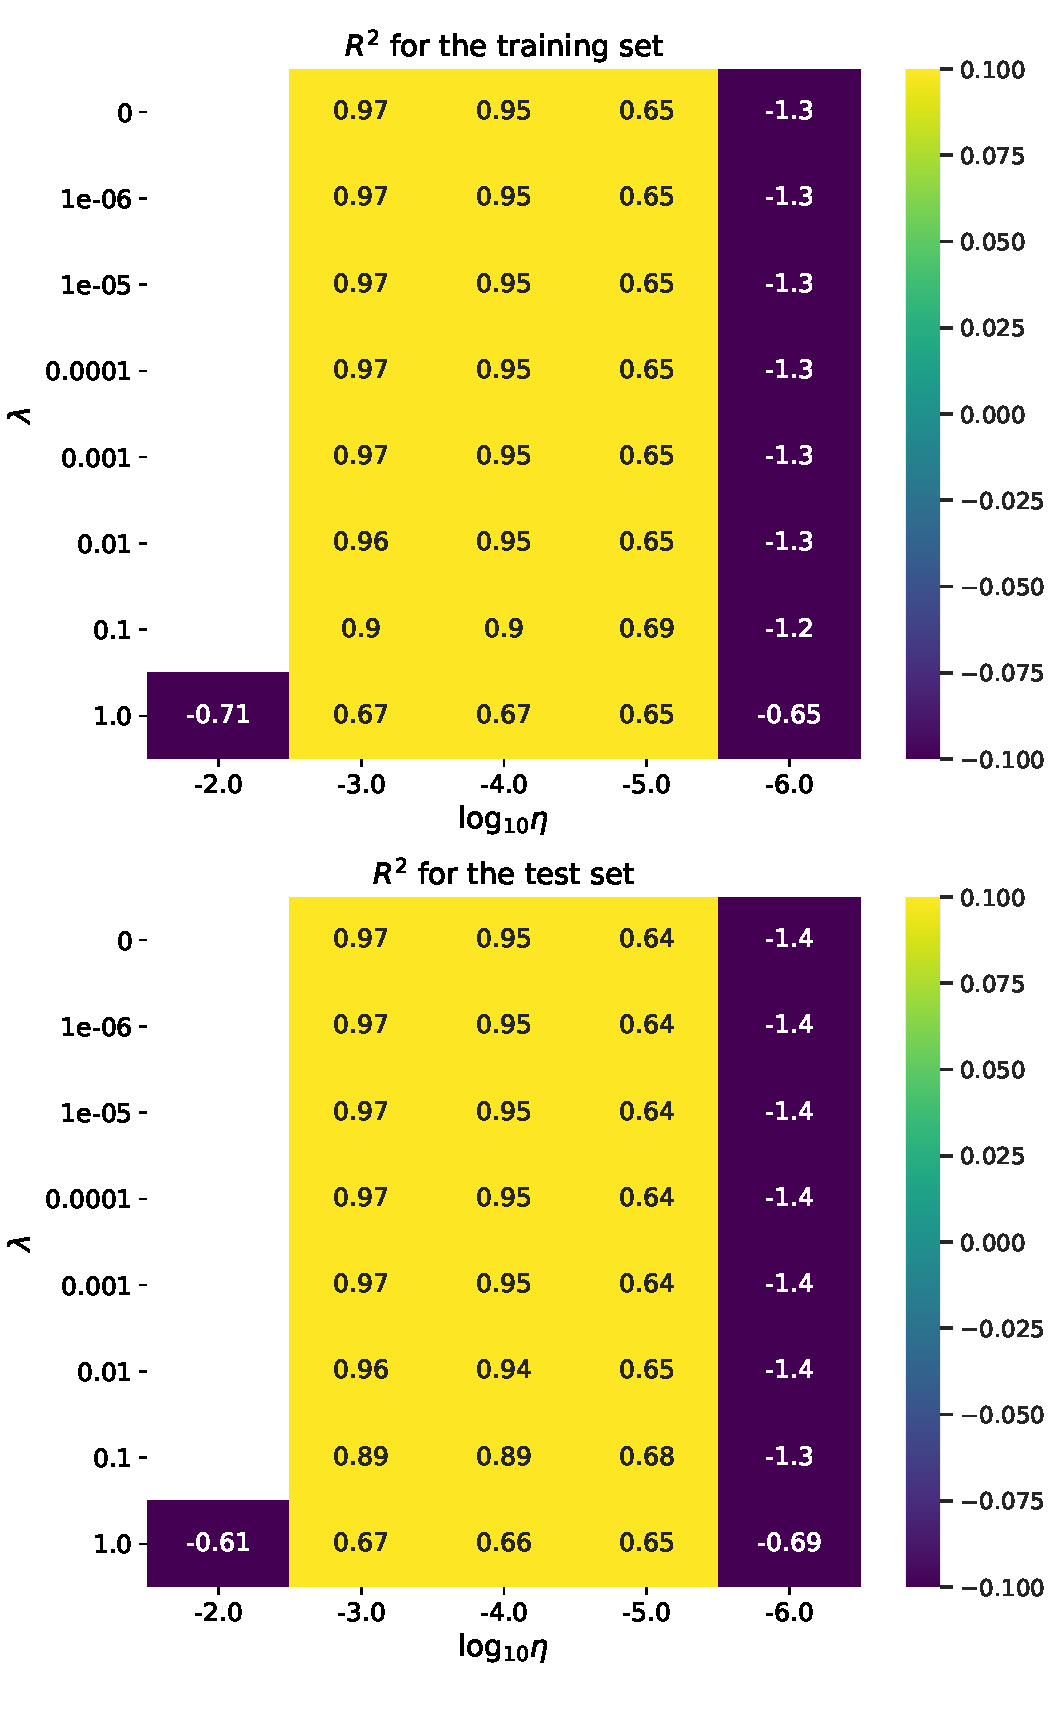
\includegraphics[width=.49\textwidth]{Figures/Ridge_R2.pdf}
    \caption{Grid search for the optimal $\lambda$ and $\eta$ maximising the training (upper panel) and test (lower panel) $R^2$ scores for Ridge with the SGD with 5-fold cross-validation, $N_{\mathrm{epochs}}=1000$, $M=5$. Coarse learning rate grid.}
    \label{fig: Ridge_grid_R2_coarse}
\end{figure}

\begin{figure}[h]
    \centering
    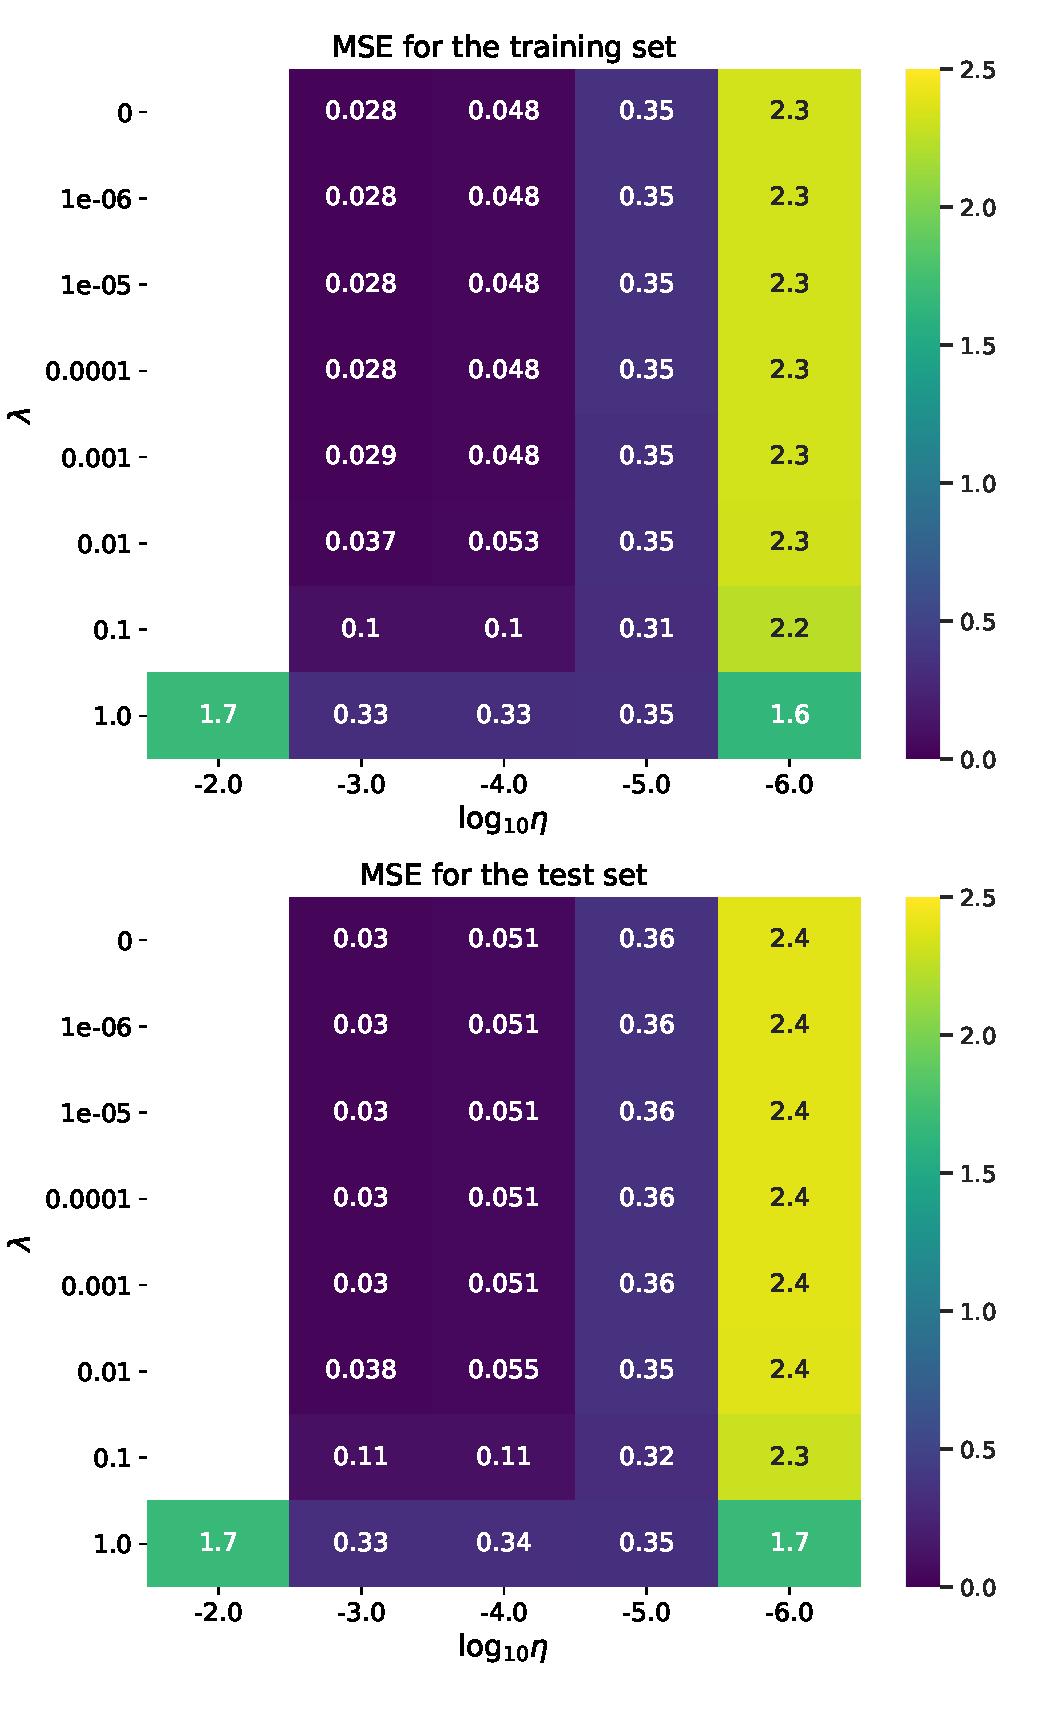
\includegraphics[width=.49\textwidth]{Figures/Ridge_MSE.pdf}
    \caption{Grid search for the optimal $\lambda$ and $\eta$ minimizing the training (upper panel) and test (lower panel) MSE for Ridge with the SGD with 5-fold cross-validation, $N_{\mathrm{epochs}}=1000$, $M=5$. Coarse learning rate grid.}
    \label{fig: Ridge_grid_MSE_coarse}
\end{figure}

\begin{figure}[h]
    \centering
    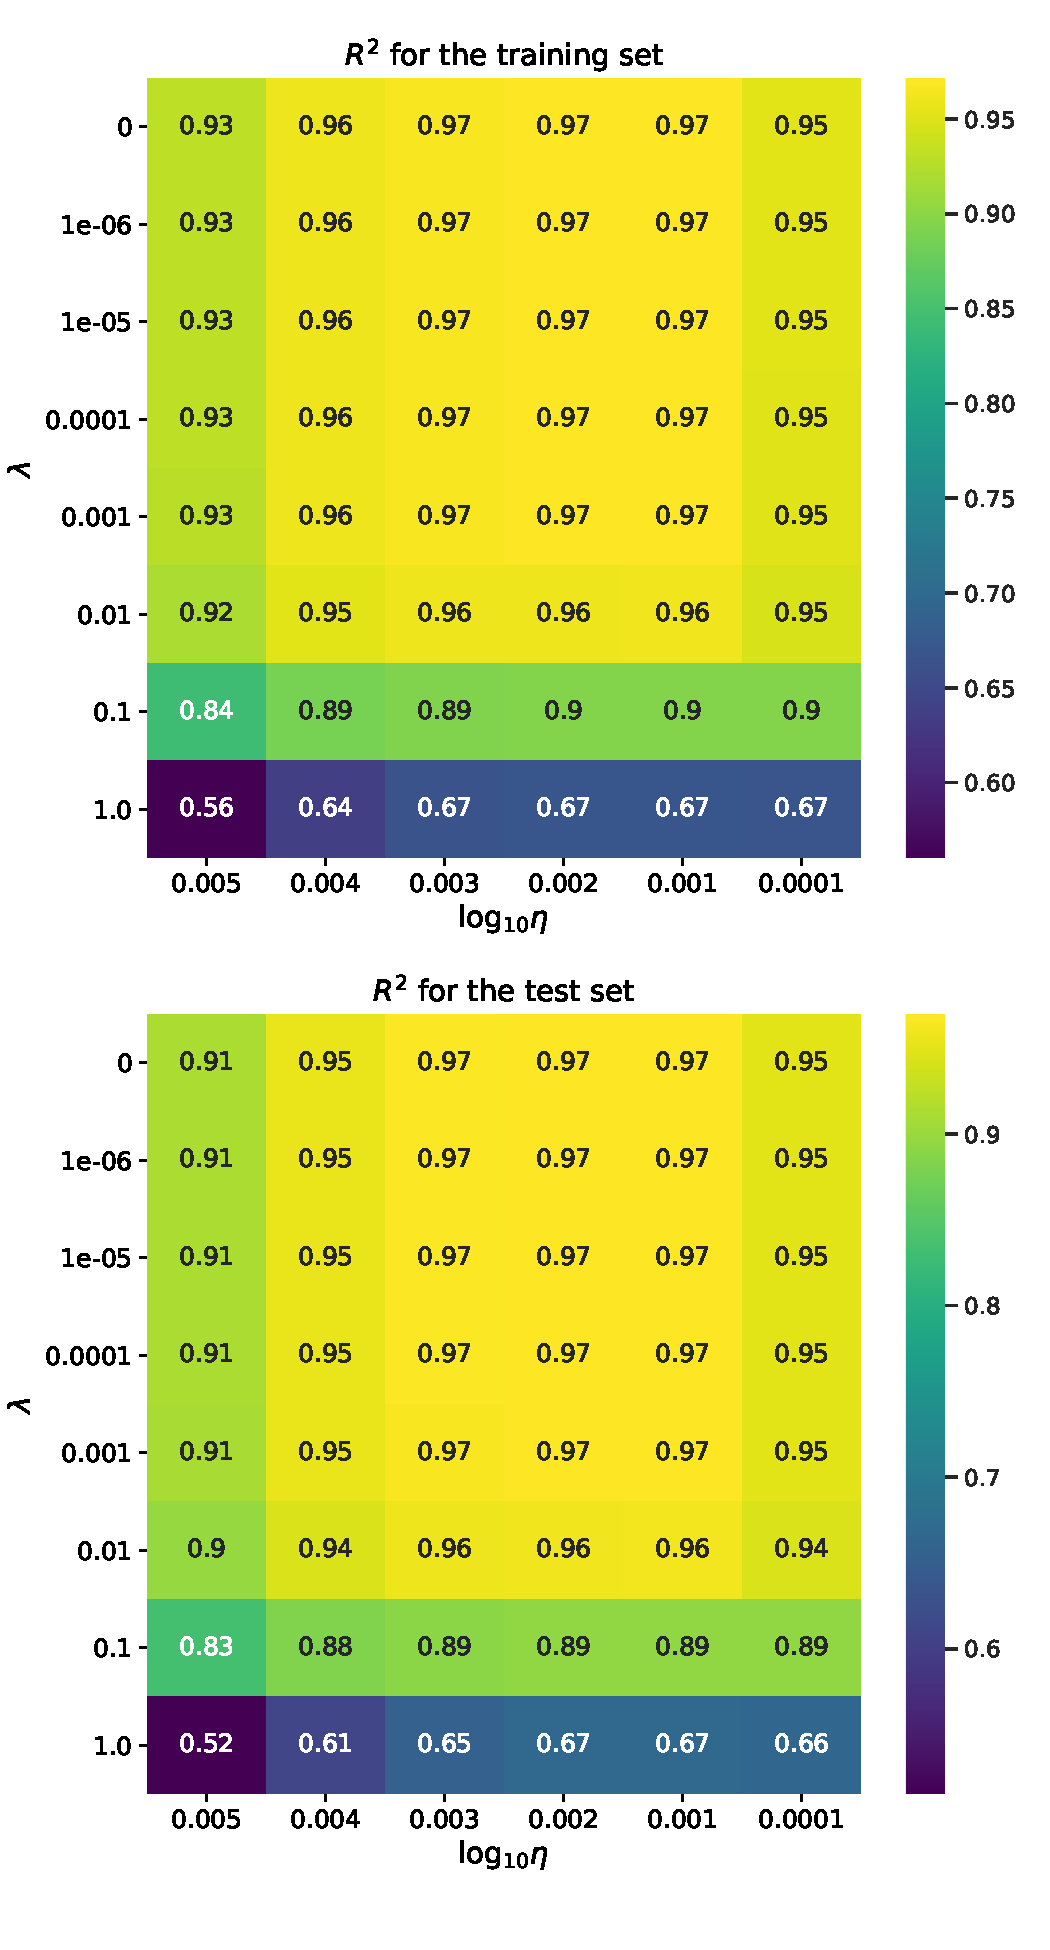
\includegraphics[width=.49\textwidth]{Figures/Ridge_R2_fine.pdf}
    \caption{Grid search for the optimal $\lambda$ and $\eta$ maximising the training (upper panel) and test (lower panel) $R^2$ scores for Ridge with the SGD with 5-fold cross-validation, $N_{\mathrm{epochs}}=1000$, $M=5$. Fine learning rate grid.}
    \label{fig: Ridge_grid_R2_fine}
\end{figure}

\begin{figure}[h]
    \centering
    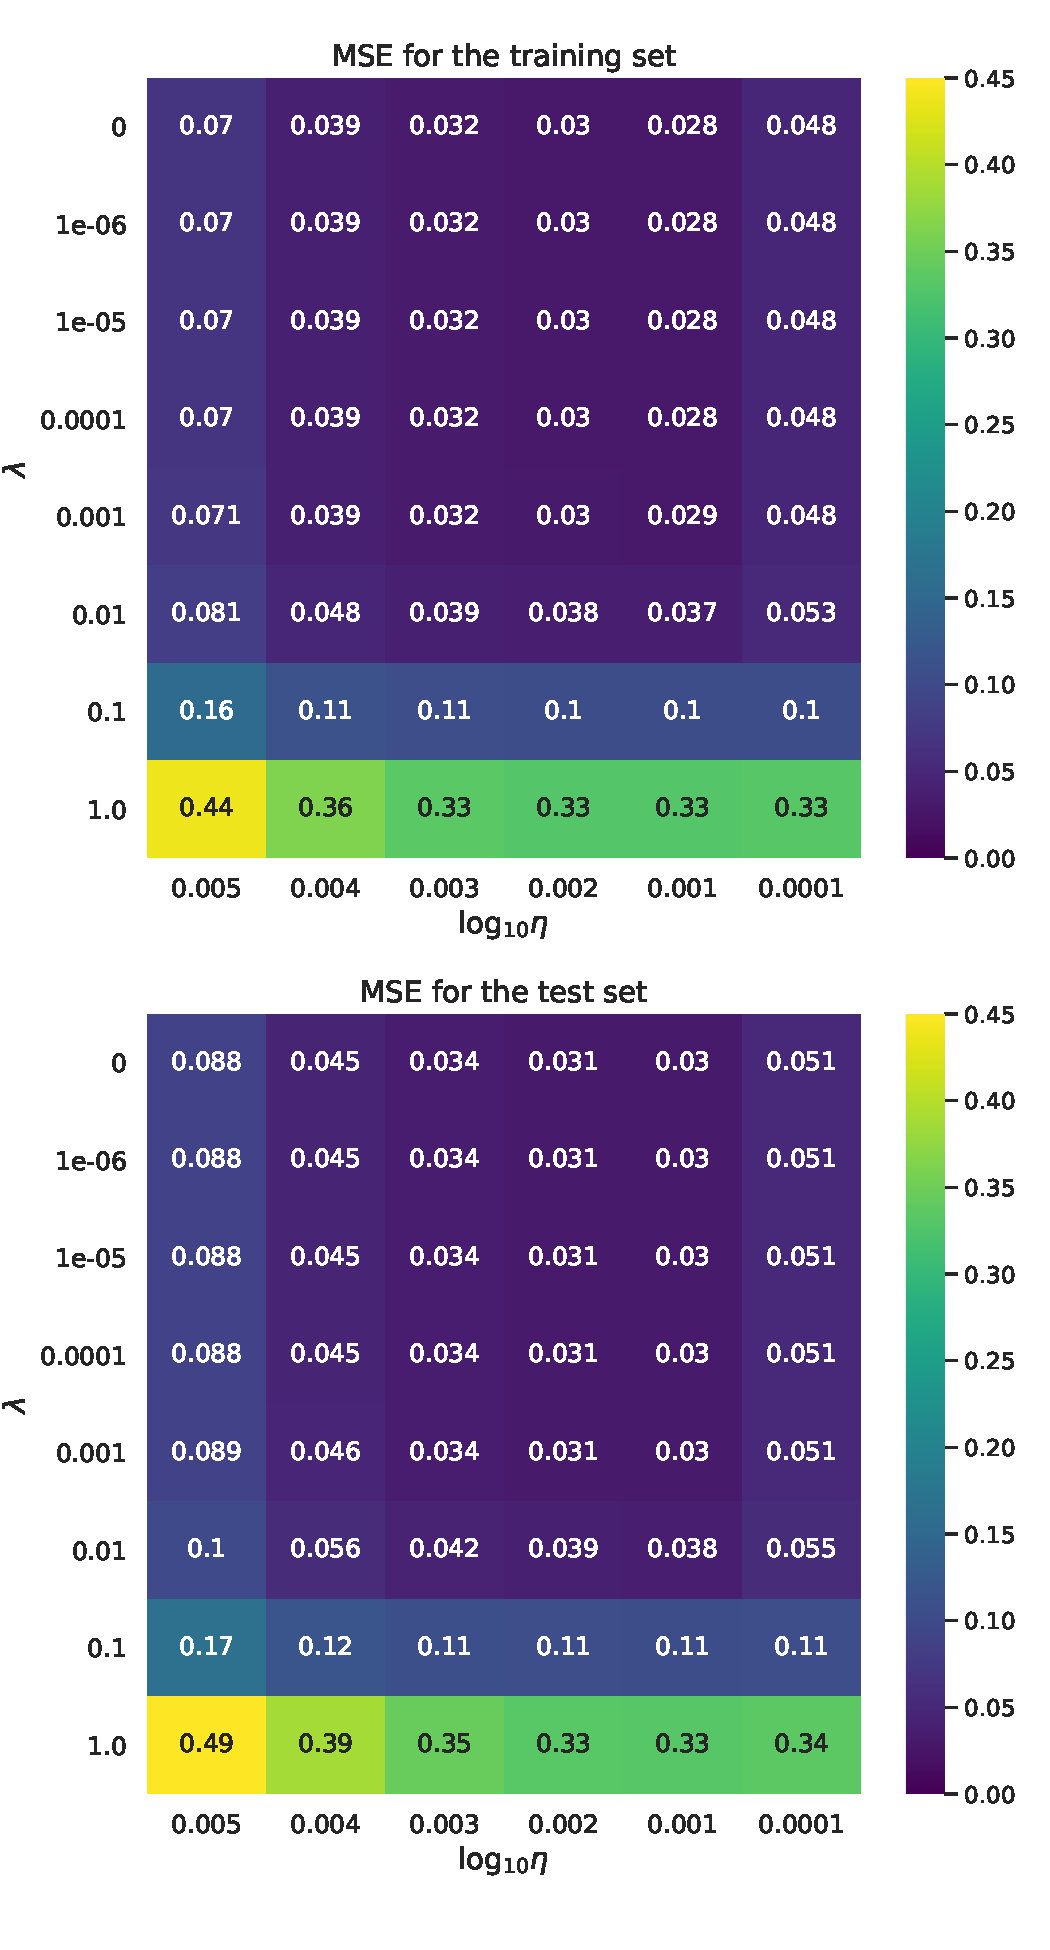
\includegraphics[width=.49\textwidth]{Figures/Ridge_MSE_fine.pdf}
    \caption{Grid search for the optimal $\lambda$ and $\eta$ minimizing the training (upper panel) and test (lower panel) MSE for Ridge with the SGD with 5-fold cross-validation, $N_{\mathrm{epochs}}=1000$, $M=5$. Fine learning rate grid.}
    \label{fig: Ridge_grid_MSE_fine}
\end{figure}

Additionally, we investigated the effects of a scaled learning rate $\eta$. As it was mentioned in Section \ref{subsubsec: SGD}, the learning rate can be set to adjustable as procedure runs through a chosen number of epochs and iterations. By scaled from now on we define the learning rate $\eta=t_0/(t_1+e\cdot m+i)$ with $e$ being a current epoch, $i$ - a current minibatch, $m$ - total number of minibatches. This adjustable learning rate starts with the initial value $t_0/t_1$ and decreases gradually with the number of epochs and minibatch number. The scaled learning rate was tested versus the constant learning rate that keeps the same value $t_0/t_1$ throughout the whole procedure. The results in Table \ref{tab:OLS} show the training and test $R^{2}$ scores and MSEs for OLS with both a constant $\eta$ and a scaled $\eta$. From these results, the performance with the constant learning rate is noticeably better and for the further analysis we should not scale the $\eta$ for OLS with the chosen parameters. From now on the learning rate is kept constant.

In Table \ref{tab:OLS vs ridge} the test $R^{2}$ score and MSE is presented for both OLS and Ridge using the matrix inversion from Project 1, as well as our SGD and and Scikit-Learn SGD (SKL SGD). We also have included the results using the standard gradient descent method. The results are presented for a selected number of different learning rates, as is shown in the Table \ref{tab:OLS vs ridge}. For the SKL SGD maximum 1000 iterations were sufficient to achieve a result comparable to the implemented SGD. For the GD 100000 were chosen and found sufficient to achieve good performance on both the training and the test set.


\begin{table}[!htb]
\begin{center}
\caption{The $R^2$ scores for the test and training datasets for the constant ($\eta=0.001$) and scaled ($t_0=1, t_1=1000$) learning rates, $N_{\mathrm{epochs}}=1000$, $M=5$, OLS case with 5-fold cross-validation.}
\label{tab:OLS}  
\begin{tabular}{lllll}
\cline{2-5}
\noalign{\smallskip}
\cline{2-5}\noalign{\smallskip}
& \multicolumn{2}{c}{Constant $\eta$} & \multicolumn{2}{c}{Scaled $\eta$}\\
\cline{2-5}\noalign{\smallskip} & Train &  Test  & Train & Test \\
\hline\noalign{\smallskip}
\multicolumn{1}{l|}{$R^2$} & 0.9716 & 0.9698 & 0.9197 & 0.9166 \\
\multicolumn{1}{l|}{MSE} & 0.0283 & 0.0301 & 0.0803 & 0.0829 \\ \noalign{\smallskip}\hline
\end{tabular}
\end{center}
\end{table}

\begin{table}[!htb]
\begin{center}
\caption{\scriptsize Comparison of the test $R^2$ for OLS ($\lambda=0.0) $ and Ridge ($\lambda=0.001$) for the standard matrix inversion, SGD with $N_{\mathrm{epochs}}=1000$ and $\eta=0.001$, GD with 100000 iterations and $\eta=0.01,0.001$, and scikit-learn SGD with $\eta=0.01,0.001$ and maximum limit of 1000 iterations. }
\label{tab:OLS vs ridge}  
\begin{tabular}{lllll}
\cline{2-5}\noalign{\smallskip}\cline{2-5}\noalign{\smallskip}
& \multicolumn{2}{c}{OLS} & \multicolumn{2}{c}{Ridge} \\ \cline{2-5}\noalign{\smallskip} 
& $R^2$ & MSE & $R^2$ & MSE \\ \hline\noalign{\smallskip}
\multicolumn{1}{l|}{Mat.inv.} & 0.9712 & 0.0287 & 0.9712 & 0.0287\\
\multicolumn{1}{l|}{SGD, $\eta=0.001$} & 0.9698 & 0.0301 & 0.9697 & 0.0302\\
\multicolumn{1}{l|}{SGD SKL, $\eta=0.01$} & 0.9398  & 0.0599 & 0.9394 & 0.0603\\
\multicolumn{1}{l|}{SGD SKL, $\eta=0.001$} & 0.8516  & 0.1480 & 0.8514 & 0.1482\\
\multicolumn{1}{l|}{GD, $\eta=0.01$} & 0.9712 & 0.0287 & 0.9710 & 0.0288\\
\multicolumn{1}{l|}{GD, $\eta=0.001$} & 0.9710 & 0.0289 & 0.9706 & 0.0292\\ \noalign{\smallskip}\hline
\end{tabular}
\end{center}
\end{table}

\subsection{Regression with Neural Networks}
\label{subsec:regression neural network}

The SGD discussed in the previous section forms the base for the learning mechanism in the neural network. As the main structure of the NN is developed, an important choice to make is to set initial guesses for all hidden layers, an output layer as well as the corresponding biases. For the NN used to produce the results in this task we have, unless stated otherwise, set the biases as small constant values, $b_i=0.01$, the weights used are normally distributed $w_{ij}\in\mathcal{N}(0,1)$, and for the output activation we simply select the identity function $f(x) = x$. For each hidden layer the Sigmoid activation function is chosen.

In Table \ref{tab:Ols vs ridge vs FFNN and NN} the results for the cases with and without regularization ($\lambda=0.001, \lambda=0$ respectively) our self-made FFNN with three hidden layers and 50 neurons in each is compared to the results obtained with the matrix inversion, the Scikit-Learn FFNN using both SGD and ADAM optimizer, and TensorFlow Keras FFNN using SGD and ADAM as optimizers. For all mentioned NN 1000 epochs, minibatch size $M=5$ and $\rta=0.001$ were chosen. For the Keras NN performance can be further improved by setting $\eta=0.01$. This result is also included in the Table \ref{tab:Ols vs ridge vs FFNN and NN}. We see that all the NN perform better than matrix inversion. For Scikit-Learn and Keras we test several different optimizers, but the Keras FFNN with ADAM seems to perform best for the case with $\lambda=0$, whereas our self-made FFNN perform the best for $\lambda=0.001$.

\begin{table}[!htb]
\begin{center}
\caption{\scriptsize The MSE and $R^2$ scores for the test set obtained for  $\lambda=0$ and $\lambda=0.001$ with matrix inversion, self-made FFNN, Scikit-learn FFNN, and Tensorflow Keras FFNN. For all NN three hidden layers with 50 neurons, $N_{\mathrm{epochs}}=1000$, $M=5$ are used. For all cases except for the Keras SGD-based NN ($\eta=0.01$), $\eta=0.001$ is used.}
\label{tab:Ols vs ridge vs FFNN and NN}  
\begin{tabular}{lllll}
\cline{2-5}\noalign{\smallskip}\cline{2-5}\noalign{\smallskip}
& \multicolumn{2}{c}{$\lambda=0$} & \multicolumn{2}{c}{$\lambda=0.001$} \\ \cline{2-5}\noalign{\smallskip} 
& $R^2$ & MSE & $R^2$ & MSE \\ \hline\noalign{\smallskip}
\multicolumn{1}{l|}{Mat.inv.} & 0.9719 & 0.0287 & 0.9719 & 0.0287\\
\multicolumn{1}{l|}{FFNN} & 0.9955 & 0.0039 & 0.9967 & 0.0028\\
\multicolumn{1}{l|}{FFNN SKL (SGD)} & 0.9908 & 0.0080 & 0.9908 & 0.0079\\
\multicolumn{1}{l|}{FFNN SKL (ADAM)} & 0.9978 & 0.0019 & 0.9965 & 0.0030\\
\multicolumn{1}{l|}{FFNN Keras (SGD), $\eta=0.01$} & 0.9983 & 0.0014 & 0.9931 & 0.0059\\
\multicolumn{1}{l|}{FFNN Keras (SGD), $\eta=0.001$} & 0.9806 & 0.0168 & 0.9682 & 0.0274\\
\multicolumn{1}{l|}{FFNN Keras (ADAM)} & 0.9999 & 0.0001 & 0.9938 & 0.0053\\
 \noalign{\smallskip}\hline
\end{tabular}
\end{center}
\end{table}

We also study how the training and test MSE behaves for our FFNN with three hidden layers for an increasing number of epochs. This result can be seen in Figure \ref{fig: NN_MSE_epochs}. An overall trend here is a decrease of the training and test MSE with increasing number of neurons. The decrease for the training set is apparent, whilst the test value varies significantly throughout the whole range chosen for the number of epochs. This makes the search for the local minimum of the test MSE complicated. In overall, we observe a slight increase of the MSE for the number of epochs higher than $\approx 900$, implying that for  $N_{\mathrm{epochs}}$ we might enter the area of overfitting.

\begin{figure}[h]
    \centering
    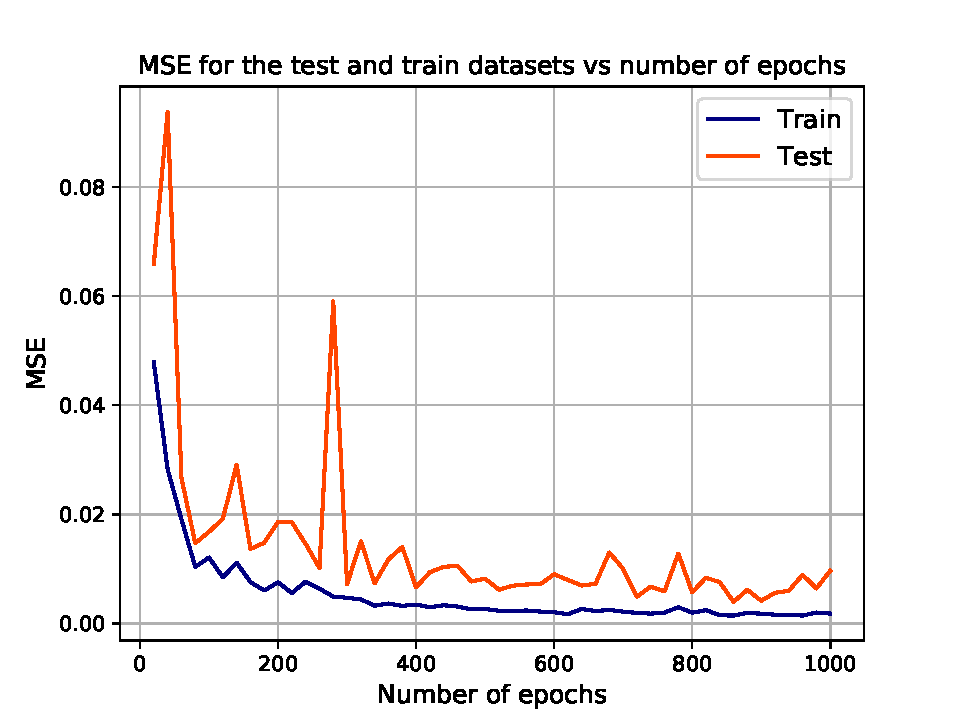
\includegraphics[width=.49\textwidth]{Figures/NN_MSE_epochs.pdf}
    \caption{Mean squared error for the test and train datasets as a function of number of epochs for the FFNN with three hidden layers with 50 neurons in each, $\eta=0.001$, $M=5$.}
    \label{fig: NN_MSE_epochs}
\end{figure}

In Fig.\ref{fig: NN_MSE_layers} we study how the MSE for the FFNN changes with increasing number of hidden layers. The decrease of the test and training MSEs is quite steady, no overfitting is observed. Adding additional hidden layers might be a clue to improving a performance of the network. Fig.\ref{fig: NN_MSE_neurons} illustrates how the MSE changes with increasing number of neurons for the FFNN with one hidden layer. As the training MSE drops firmly to its minimum value with the increasing number of neurons, the test MSE demonstrates significant variation from point to point. This, again makes estimation of where the networks begins to overfit the data quite unclear. In overall, one might conclude that overfitting occurs for the number of neurons bigger that $\approx20$, as the test MSE tends to increase in overall after this point. 

\begin{figure}[h]
    \centering
    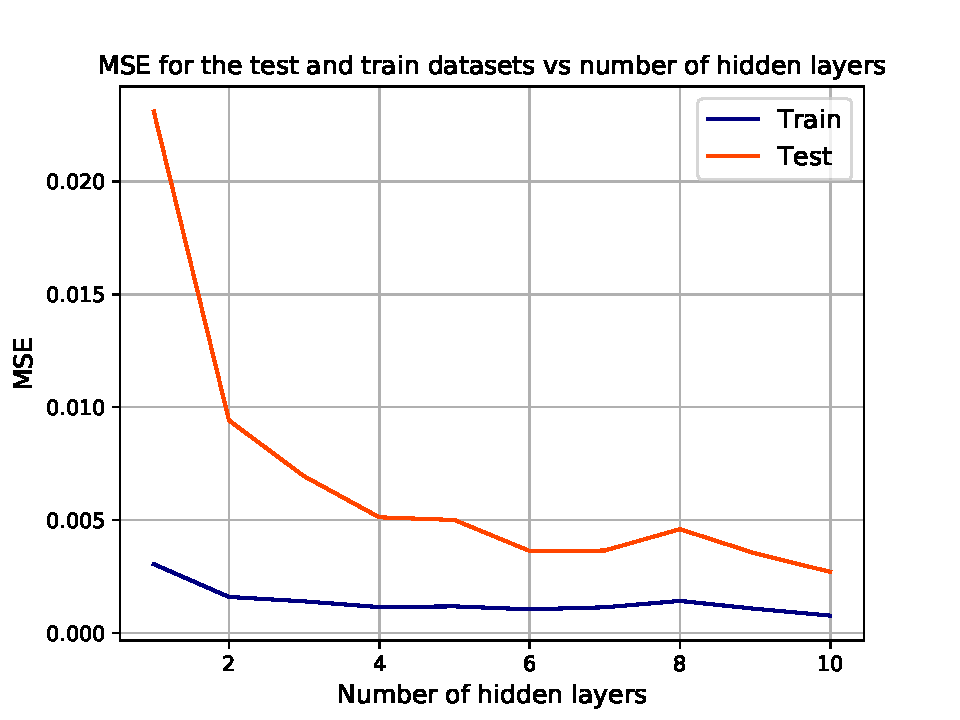
\includegraphics[width=.49\textwidth]{Figures/NN_MSE_layers.pdf}
    \caption{Mean squared error for the test and train datasets as a function of number of hidden layers (50 neurons in each) for the FFNN with $N_{epoch}=1000$, $\eta=0.001$, $M=5$.}
    \label{fig: NN_MSE_layers}
\end{figure}

\begin{figure}[h]
    \centering
    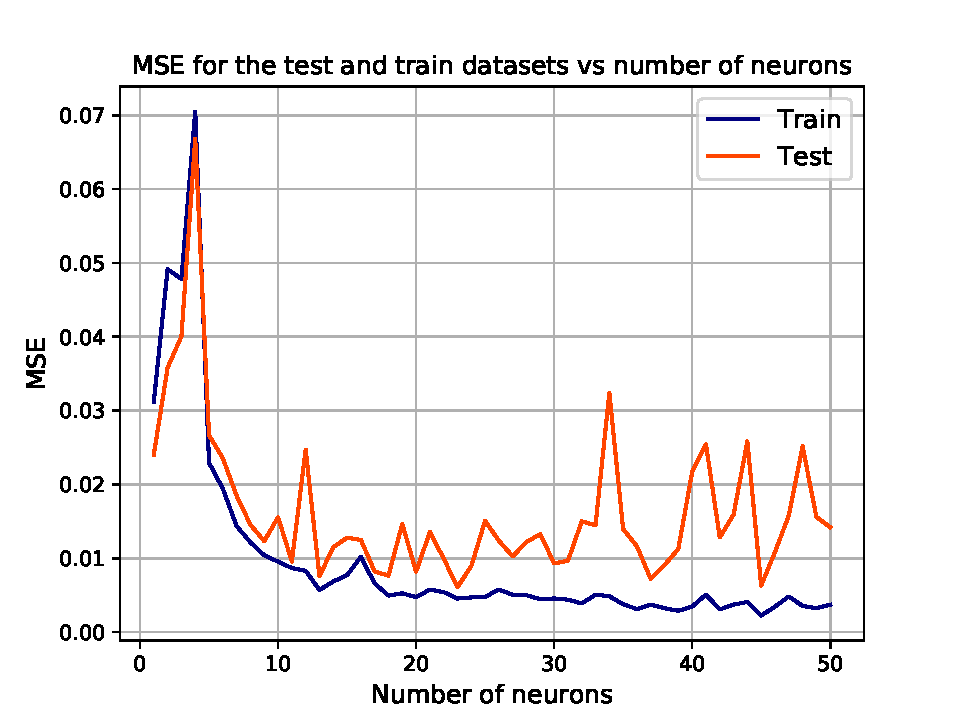
\includegraphics[width=.49\textwidth]{Figures/NN_MSE_neurons.pdf}
    \caption{Mean squared error for the test and train datasets as a function of number of neurons for the FFNN with $N_{epoch}=1000$, $\eta=0.001$, $M=5$ and one hidden layer.}
    \label{fig: NN_MSE_neurons}
\end{figure}

For the case with non-zero regularization parameter included, the grid search showing the training and test $R^{2}$ scores are found in Figure \ref{fig: NN_Ridge_R2}. Since the corresponding search for the minimum MSE is quite similar to search for the maximum $R^{2}$ scores, we present here results for $R^{2}$ only, while the grid search for the smallest test and train MSE can be found in Appendix C \ref{Appendix:C}. The blank squares denote the cases resulting in the computational overflow. The area of the highest scores for both the test and training $R^{2}$ is clear and covers $\lambda=0$ and $\lambda<0.001$ and $10^{-4}\eta<10^{-2}$.

Fig.\ref{fig:franke} demonstrates the original form of the Franke's function to be fitted (a), the fit result with the FFNN with three layers on the training data (b) and, finally, the fitted test data (c). An overall fit of both datasets is quite satisfying, which is supported by the high $R^2$ scores, stored in the Table \ref{tab:Ols vs ridge vs FFNN and NN}.

\begin{figure*}
\label{fig:franke}
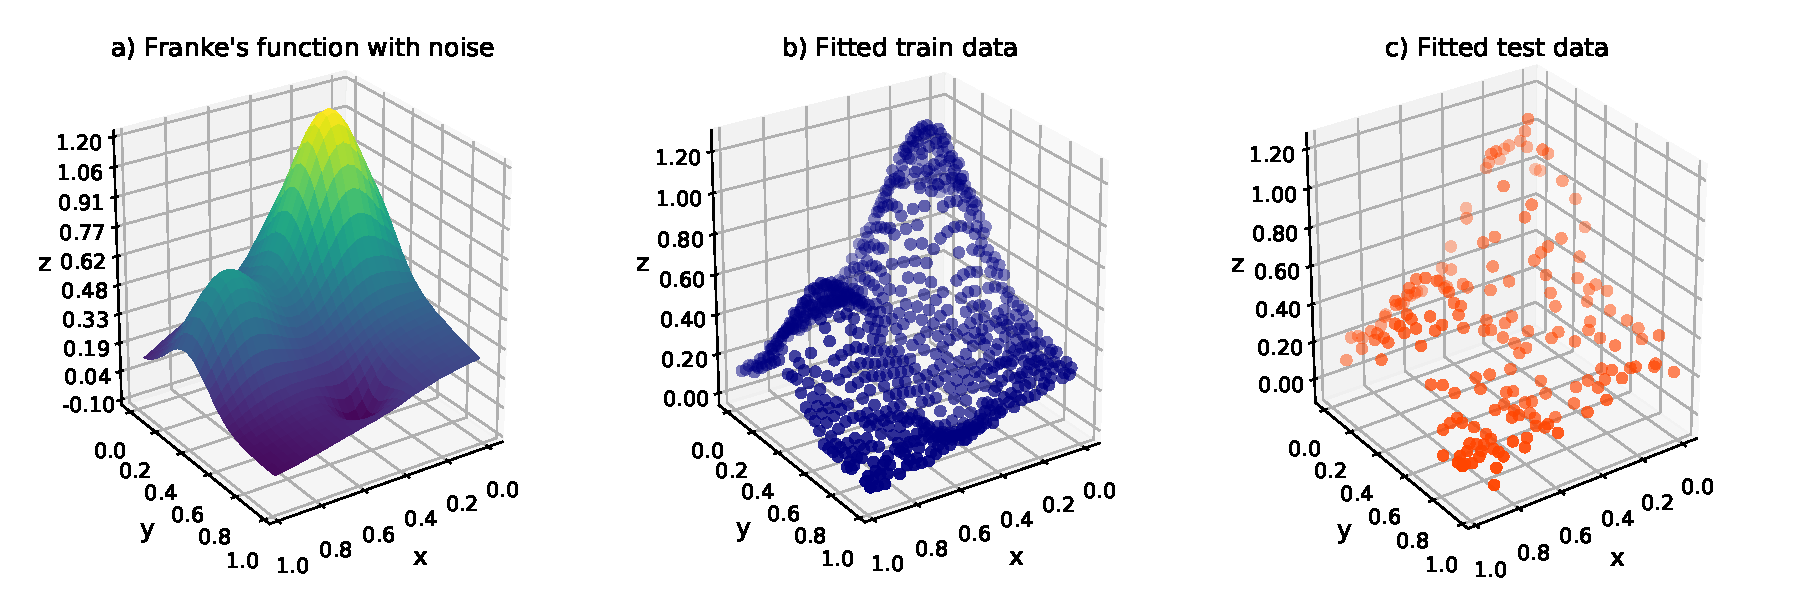
\includegraphics[width=1.0\textwidth]{Figures/Franke.pdf}% Here is how to import EPS art
\caption{\label{fig:Franke}Franke's function, test and training datasets in case of $N=30$, and total number of $(x_i,y_i)$ data pairs $N\times N=900$.}
\end{figure*}

\begin{figure}[h]
    \centering
    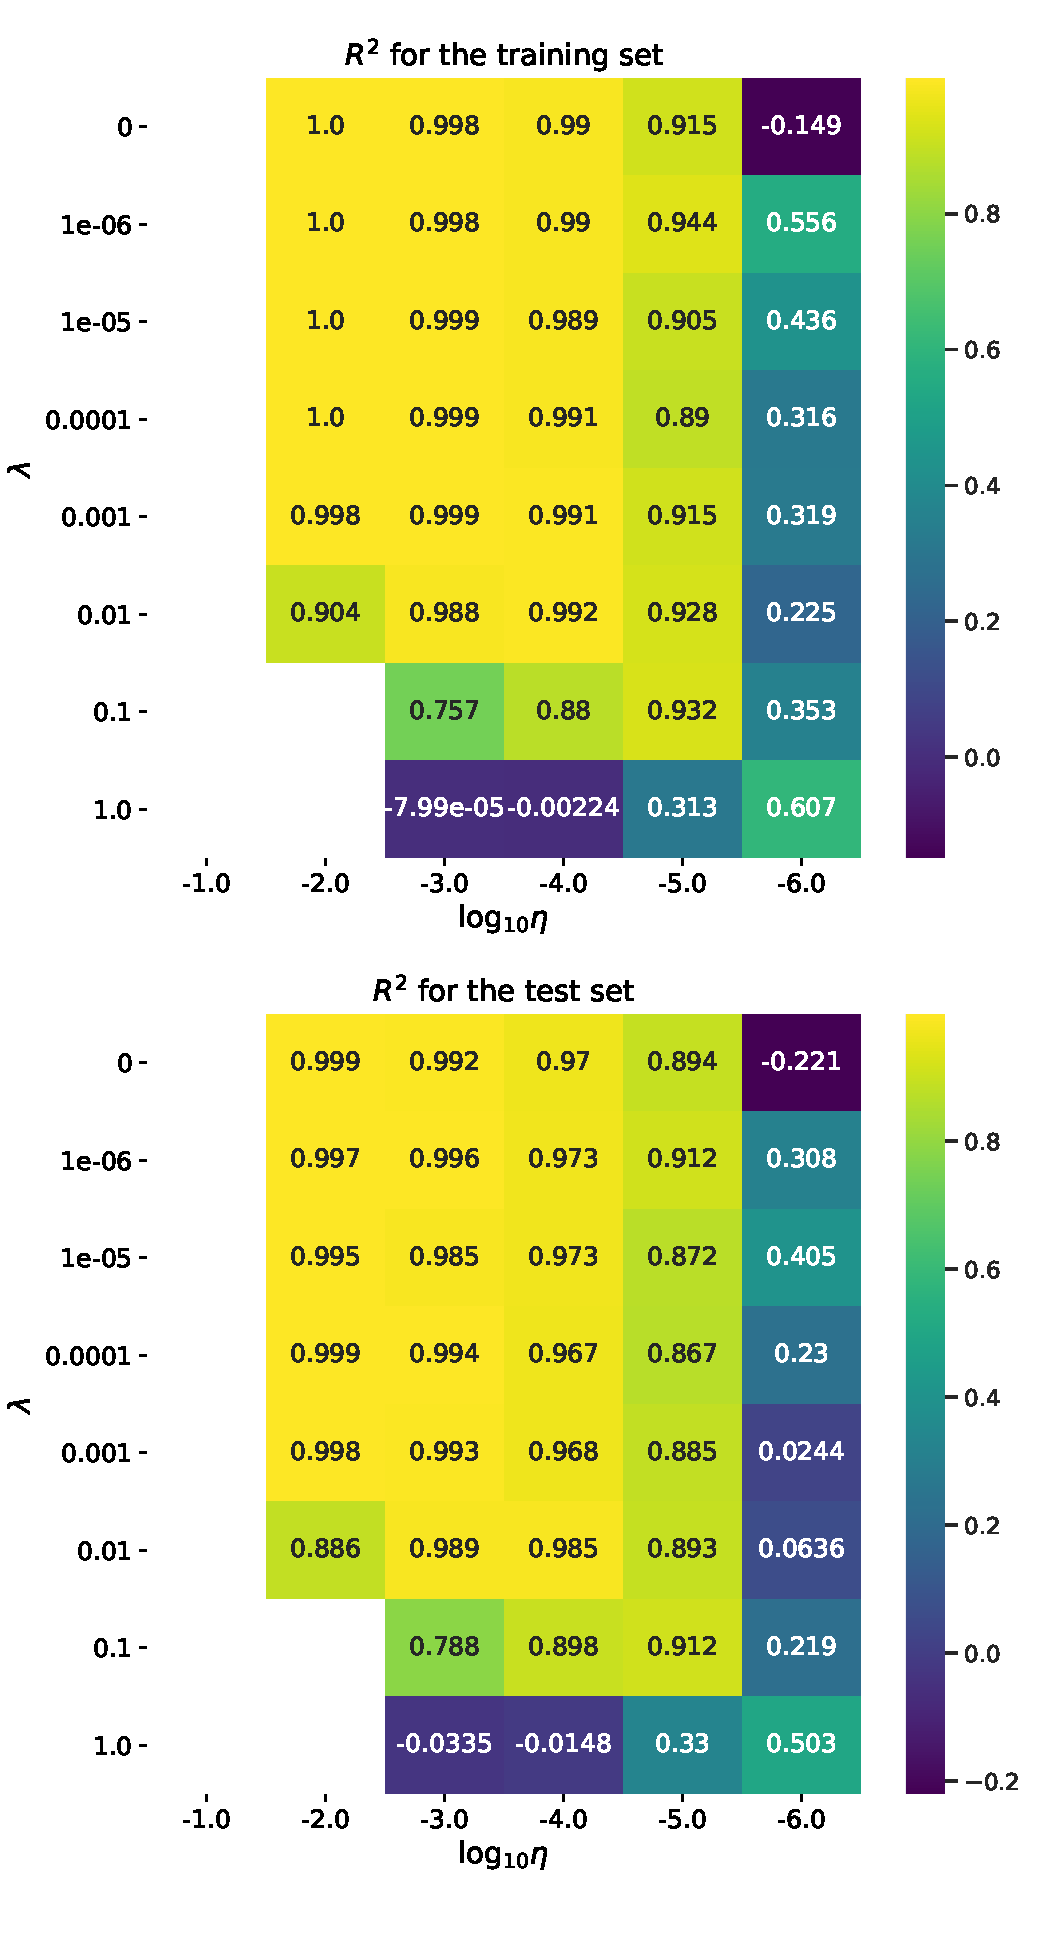
\includegraphics[width=.49\textwidth]{Figures/NN_Ridge_R2.pdf}
    \caption{Grid search for the optimal $\lambda$ and $\eta$ maximising the training (upper panel) and test (lower panel) $R^2$ scores for the three-layer FFNN (50 neurons each), $N_{\mathrm{epochs}}=1000$, $M=5$.}
    \label{fig: NN_Ridge_R2}
\end{figure}


To study how the different activation functions and initial weights and biases impact the results we hereby vary these. In Table \ref{tab:activation functions} we have used one hidden layer with 50 neurons, but calculated the $R^{2}$ score and MSE using different activation functions, namely Sigmoid, ReLU, leaky ReLU and tanh. For the leaky ReLu we present the results for two slopes below zero, $a=0.01$ and $a=0.001$. For the case of Sigmoid and tanh the NN was run with 1000 epochs, $\eta=0.001$ and minibatch size $M=5$. For the ReLU and leaky ReLU these parameters result in a computational overflow. Decreasing the learning rate was found to be a clue to overcome this issue, among $10^{-3},10^{-4},10^{-5}$, $\eta=10^{-5}$ is the first value that can be used to produce the results. In order to achieve the same performance as for the Sigmoid and tanh, the number of epochs had to be increased significantly to 100000, increasing the CPU run time dramatically. With these parameters, all activation functions performed in a very similar way, but the Sigmoid function performed slightly better than the rest. 


Another interesting aspect to study is to check influence of initial setting of weights and biases in the hidden layers, an output layer and biases. The results of how the weights and bias alter the test and training $R^{2}$ score and MSE are shown in Table \ref{tab:bias and weight FFNN}. These results seem to show that the most drastic change is when we use a constant weights ($w_{ij}=0.1$). Increasing of the bias by one order of magnitude does not seem to distort the results dramatically. The combination of constant weights and increased constant bias provided results that are a lot poorer than the results for normally distributed weights and the smaller biases. 

\begin{table}[!htb]
\begin{center}
\caption{1 hidden layer. The MSE and $R^2$ scores for the test and training datasets for the FFNN, in case of sigmoid 1000 epochs are used, $\eta=0.001$, ReLU and leaky Relu 100000 epochs, $\eta=0.00001$ }
\label{tab:activation functions}  
\begin{tabular}{lllll}
\cline{2-5}
\noalign{\smallskip}
\cline{2-5}\noalign{\smallskip}
& \multicolumn{2}{c}{$R^2$} & \multicolumn{2}{c}{MSE}\\
\cline{2-5}\noalign{\smallskip} & Train &  Test  & Train & Test \\
\hline\noalign{\smallskip}
\multicolumn{1}{l|}{Sigmoid} & 0.9970 & 0.9733 & 0.0030 & 0.0231 \\
\multicolumn{1}{l|}{ReLU} & 0.9962 & 0.9686 & 0.0039 & 0.0271 \\
\multicolumn{1}{l|}{Leaky ReLU, $a=0.001$} & 0.9962 & 0.9687 & 0.0039 & 0.0270\\
\multicolumn{1}{l|}{Leaky ReLU, $a=0.01$} & 0.9963 & 0.9686 & 0.0038 & 0.0271\\
\multicolumn{1}{l|}{tanh} & 0.9962 & 0.8942 & 0.0039 & 0.0913
\\\noalign{\smallskip}\hline
\end{tabular}
\end{center}
\end{table}

\begin{table}[!htb]
\begin{center}
\caption{The MSE and $R^2$ scores for the test and training datasets for the FFNN with $N_{epoch}=1000$, $\eta=0.001$, $M=5$. Four different ways to set initial weights and biases for the case of $\lambda=0.0$.}
\label{tab:bias and weight FFNN}  
\begin{tabular}{lllll}
\cline{2-5}
\noalign{\smallskip}
\cline{2-5}\noalign{\smallskip}
& \multicolumn{2}{c}{$R^2$} & \multicolumn{2}{c}{MSE}\\
\cline{2-5}\noalign{\smallskip} & Train &  Test  & Train & Test \\
\hline\noalign{\smallskip}
\multicolumn{1}{l|}{Normal $w_{ij}$, $b_i=0.01$} & 0.9988 & 0.9955 & 0.0013 & 0.0039 \\
\multicolumn{1}{l|}{Normal $w_{ij}$, $b_i=0.1$} & 0.9986 & 0.9945 & 0.0014 & 0.0047 \\
\multicolumn{1}{l|}{$w_{ij}=0.1$, $b_i=0.01$} & 0.8167 & 0.8281 & 0.1886 &  0.1484\\
\multicolumn{1}{l|}{$w_{ij}=0.1$, $b_i=0.1$} & 0.6294 & 0.6315 & 0.3813 & 0.3182 \\\noalign{\smallskip}\hline
\end{tabular}
\end{center}
\end{table}

\subsection{Classification}
\label{sec:classification}

For classification tasks we use primarily the Softmax function as the activation function. To estimate the performance of the neural networks we use the accuracy. 

The classification problem studied in the present work is the MNIST dataset of handwritten digits. As the neural network is trained with the dataset, we can find its accuracy for recognizing what number a handwritten digit is. 

In Figures \ref{fig:accuracy vs hidden layers}, \ref{fig:accuracy vs num neurons} and \ref{fig:accuracy vs num epochs} it is shown how the accuracy changes as a function of number of hidden layers, number of neurons, and number of epochs, respectively. We see that for our parameters we get the best accuracy for number of hidden layers at 5 and below. The accuracy is also best for number of neurons above approximately 15. As for number of epochs, we see that the accuracy is best for approximately 100 epochs, and does not improve for higher numbers. 


\begin{figure}[h]
    \centering
    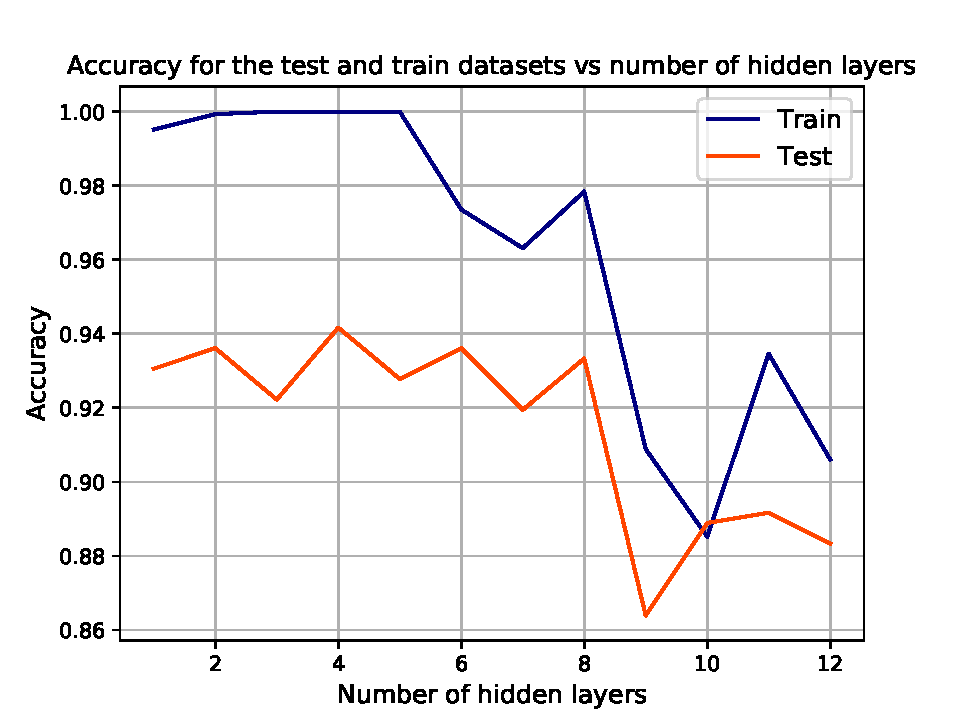
\includegraphics[width=.49\textwidth]{Figures/Class_hidden_layers.pdf}
    \caption{Accuracy for the test and training sets as functions of the number of hidden layers, 50 neurons in each layer, 100 epochs, $\lambda=0.0$, $\eta=0.01$, minibatch size $M=50$.}
    \label{fig:accuracy vs hidden layers}
\end{figure}

\begin{figure}[h]
    \centering
    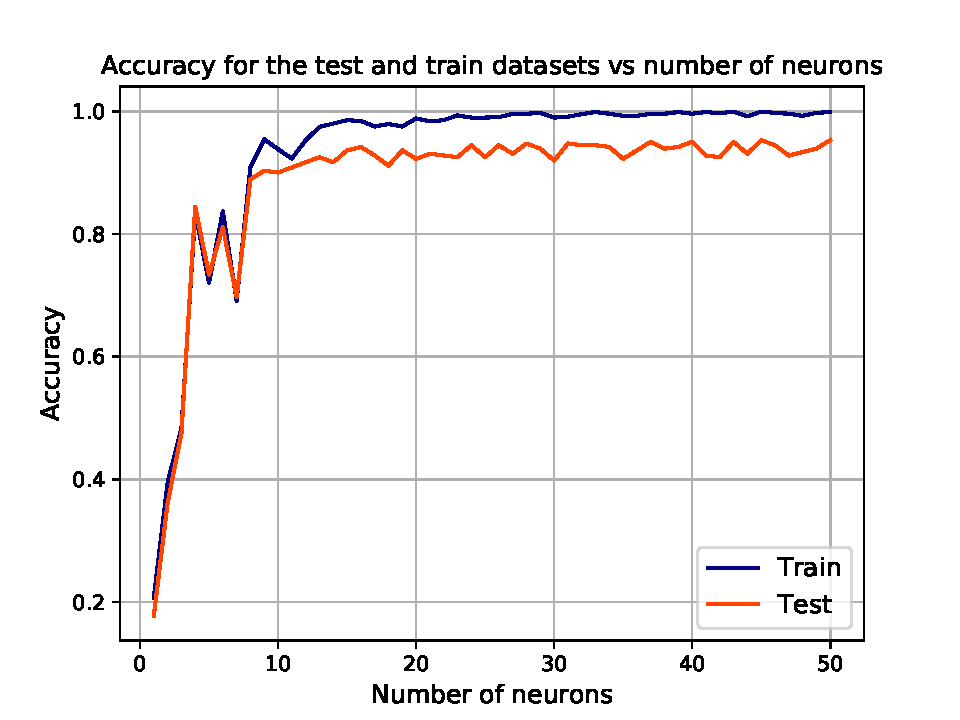
\includegraphics[width=.49\textwidth]{Figures/Class_hidden_neurons.pdf}
    \caption{Accuracy for the test and training sets as functions of the number of neurons, 1 hidden layer, 100 epochs, $\lambda=0.0$, $\eta=0.01$, minibatch size $M=50$.}
    \label{fig:accuracy vs num neurons}
\end{figure}

\begin{figure}[h]
    \centering
    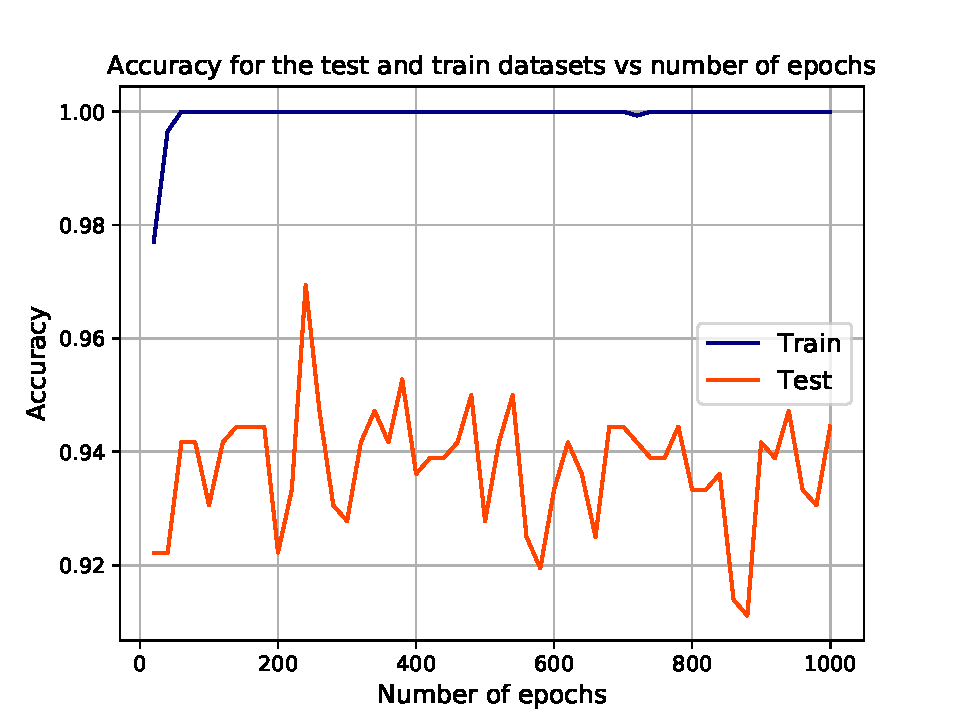
\includegraphics[width=.49\textwidth]{Figures/Class_epochs_number.pdf}
    \caption{Accuracy for the test and training sets as functions of the number of neurons, 3 hidden layers, $\lambda=0.0$, $\eta=0.01$, minibatch size $M=50$.}
    \label{fig:accuracy vs num epochs}
\end{figure}

In order to find the parameters for which we achieve the optimal accuracy, we perform a grid search. The results for the FFNN with Sigmoid activation function can be found in Figure \ref{fig: grid search class 1 layer}.

\begin{figure}[h]
    \centering
    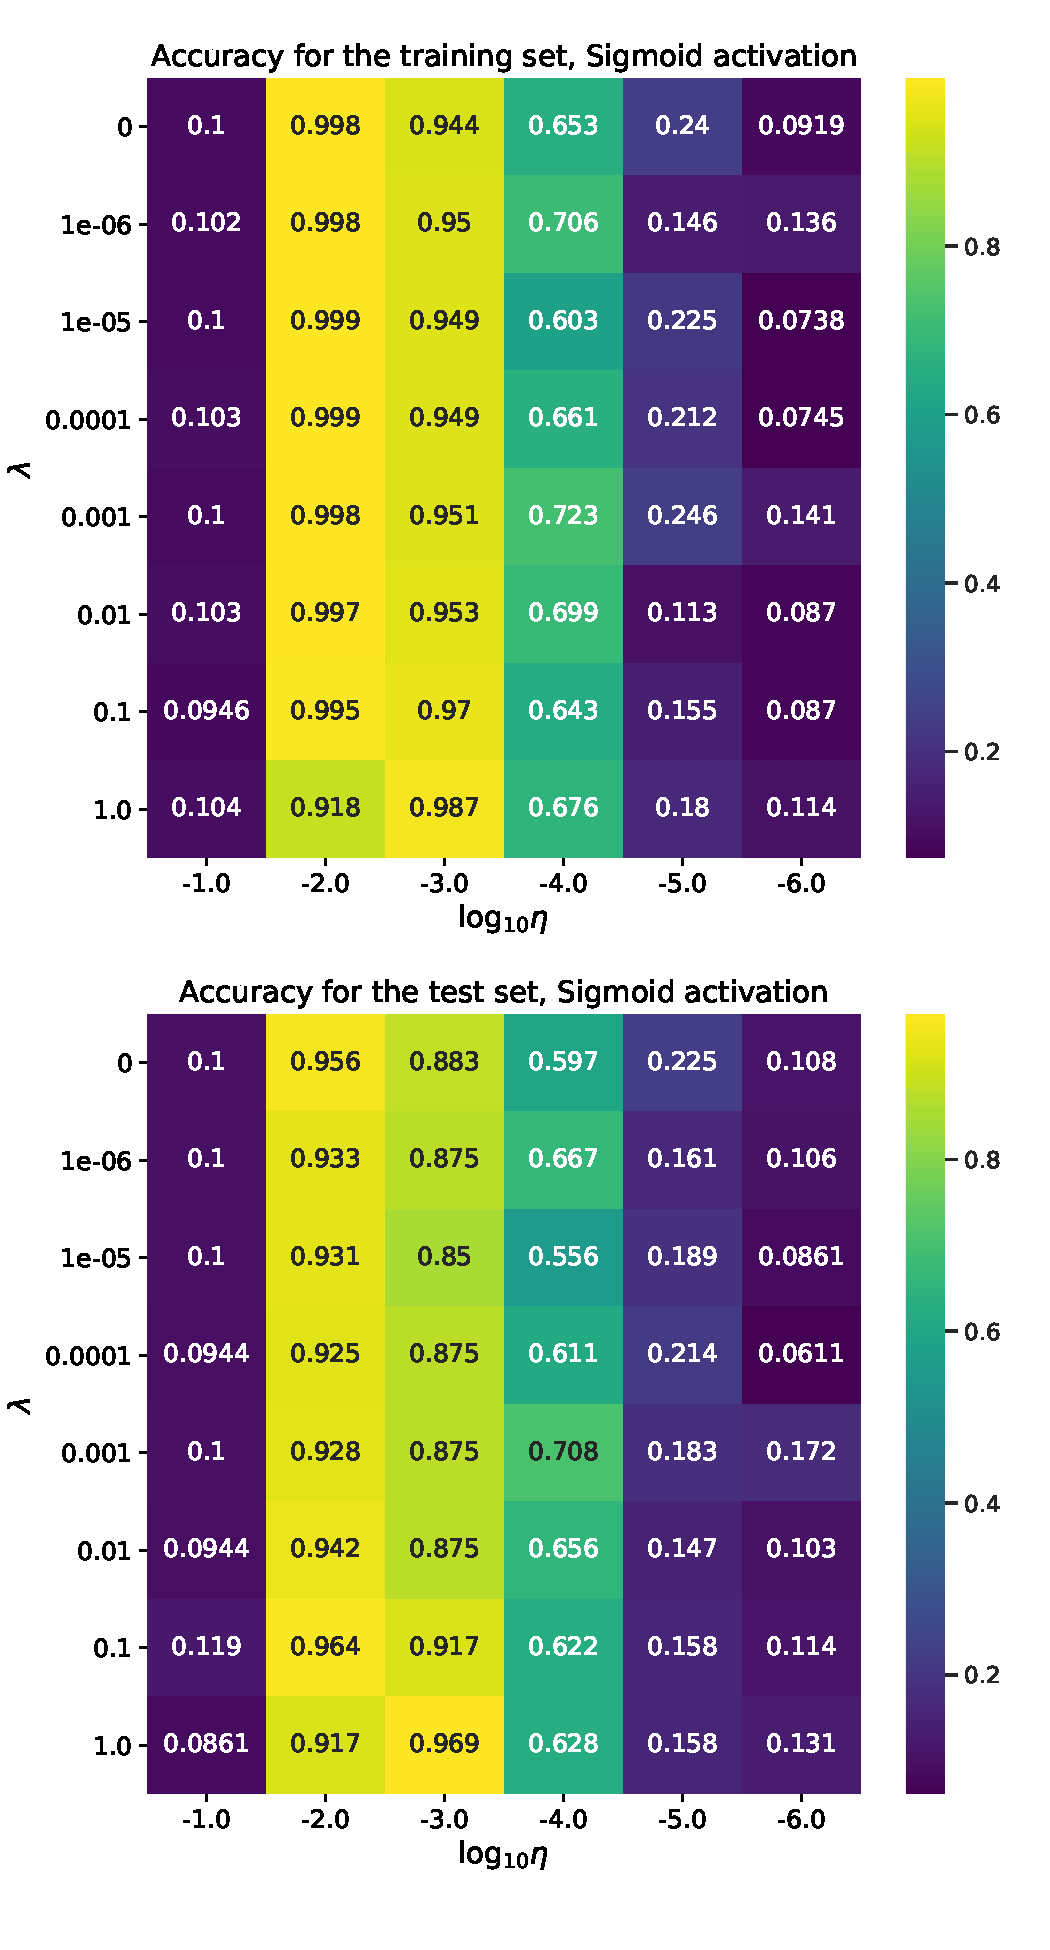
\includegraphics[width=.49\textwidth]{Figures/Class_Ridge_1_layer.pdf}
    \caption{Grid search for the optimal accuracy for the test and training sets presented as a functions of the learning rate and regularization parameter $\lambda$, 100 epochs, $M=50$. One hidden layer with Sigmoid activation function and 50 neurons is used.}
    \label{fig: grid search class 1 layer}
\end{figure}

Comparatively, the ReLU and Leaky ReLU activation functions proved to be more sensitive to input parameters. This can be seen in Figures \ref{fig: grid search class 1 layer relu} and \ref{fig: grid search class 1 layer leaky relu}. Additionally we used the tanh activation function for comparison. The results from this is presented in Figure \ref{fig: grid search class 1 layer tanh}. 

\begin{figure}[h]
    \centering
    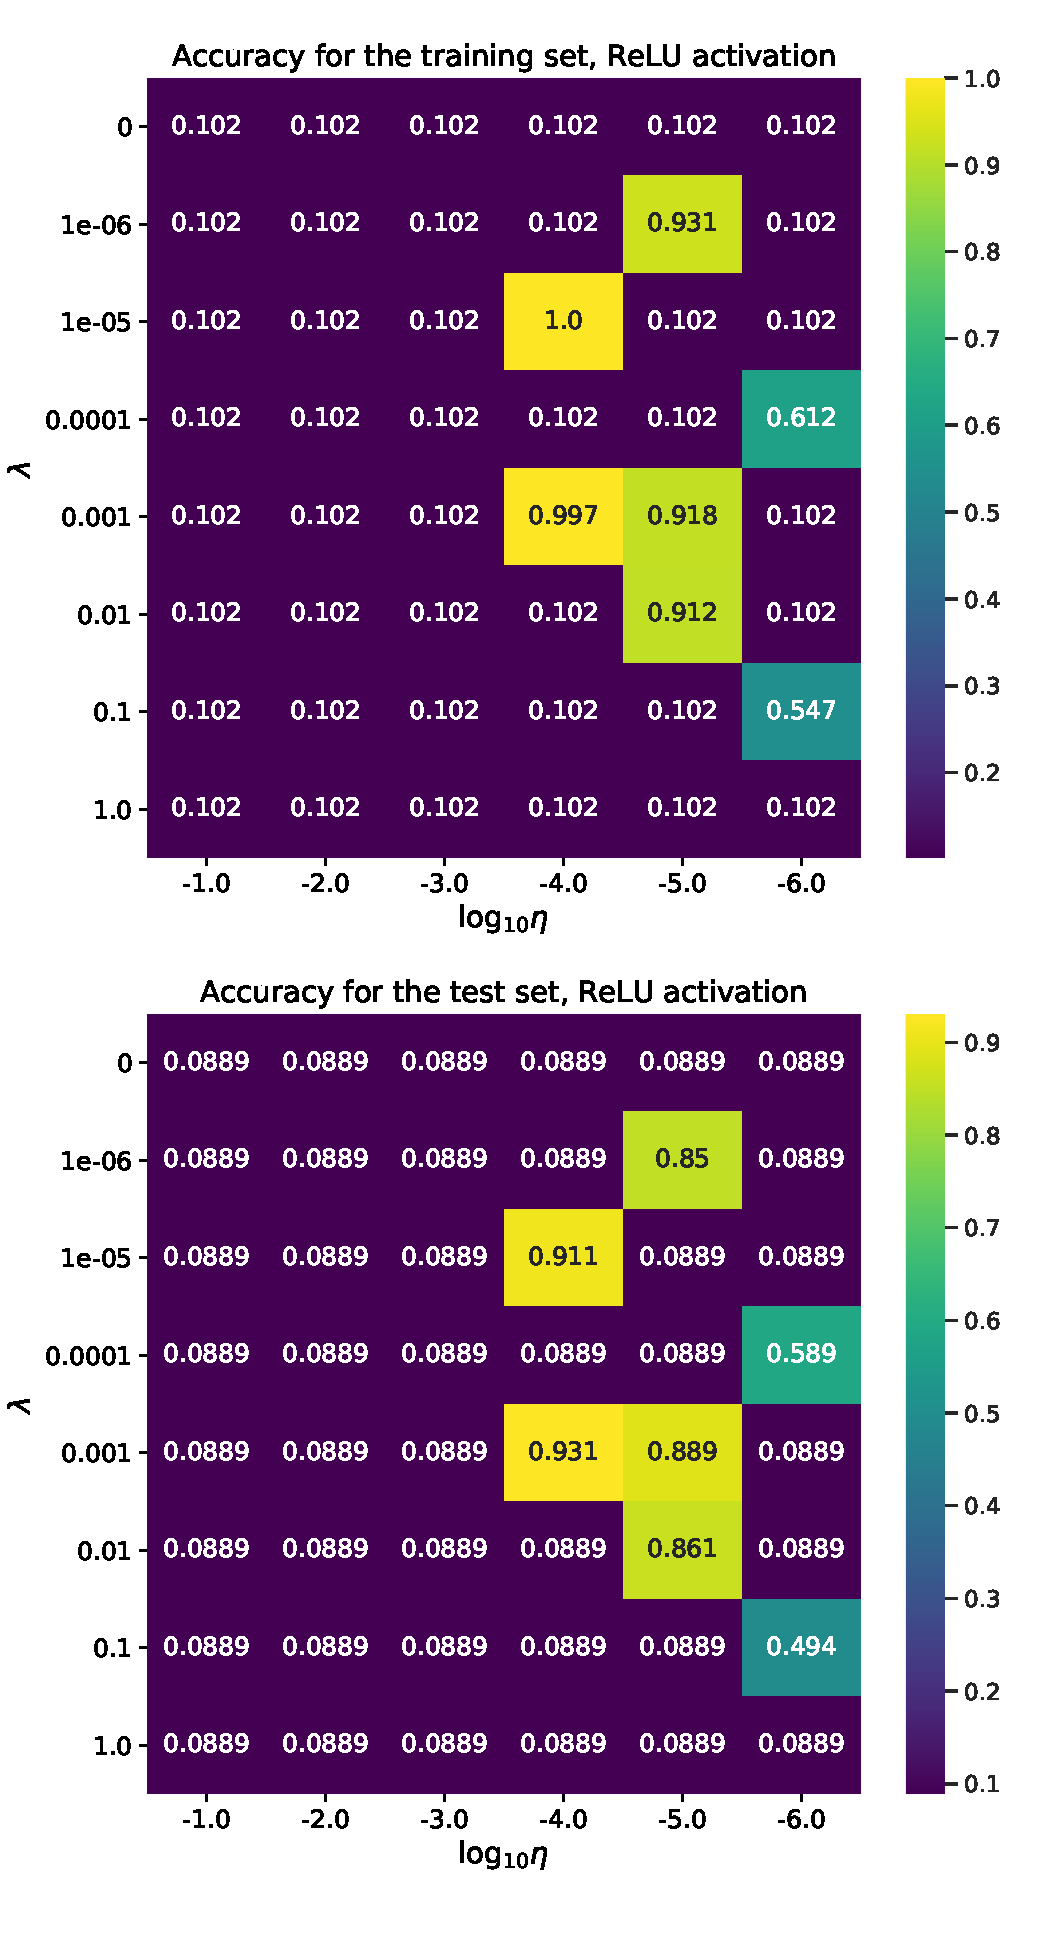
\includegraphics[width=.49\textwidth]{Figures/Class_Ridge_1_layer_relu.pdf}
    \caption{Grid search for the optimal accuracy for the test and training sets presented as a functions of the learning rate and regularization parameter $\lambda$, 100 epochs, $M=50$. One hidden layer with ReLU activation function and 50 neurons is used.}
    \label{fig: grid search class 1 layer relu}
\end{figure}

\begin{figure}[h]
    \centering
    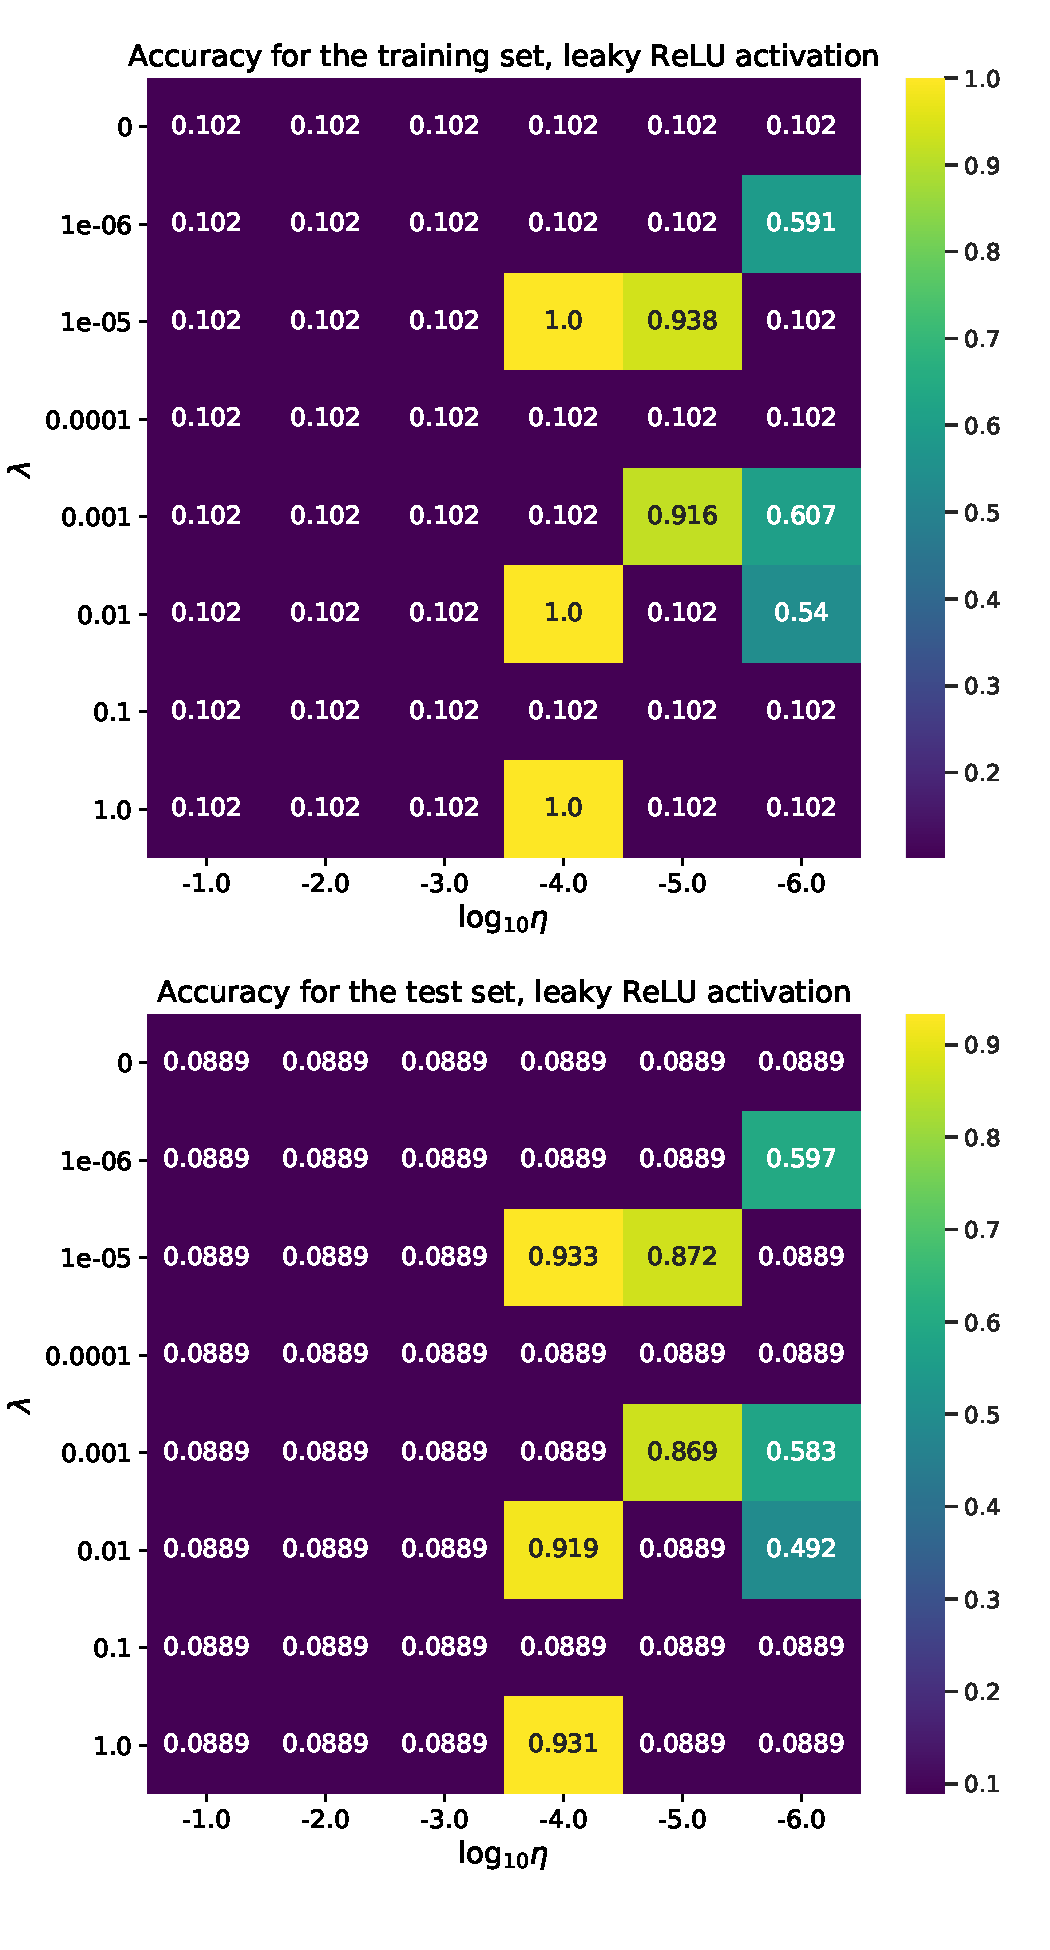
\includegraphics[width=.49\textwidth]{Figures/Class_Ridge_1_layer_leaky_relu.pdf}
    \caption{Grid search for the optimal accuracy for the test and training sets presented as a functions of the learning rate and regularization parameter $\lambda$, 100 epochs, $M=50$. One hidden layer with leaky ReLU activation function ($a=0.001$) and 50 neurons is used.}
    \label{fig: grid search class 1 layer leaky relu}
\end{figure}

\begin{figure}[h]
    \centering
    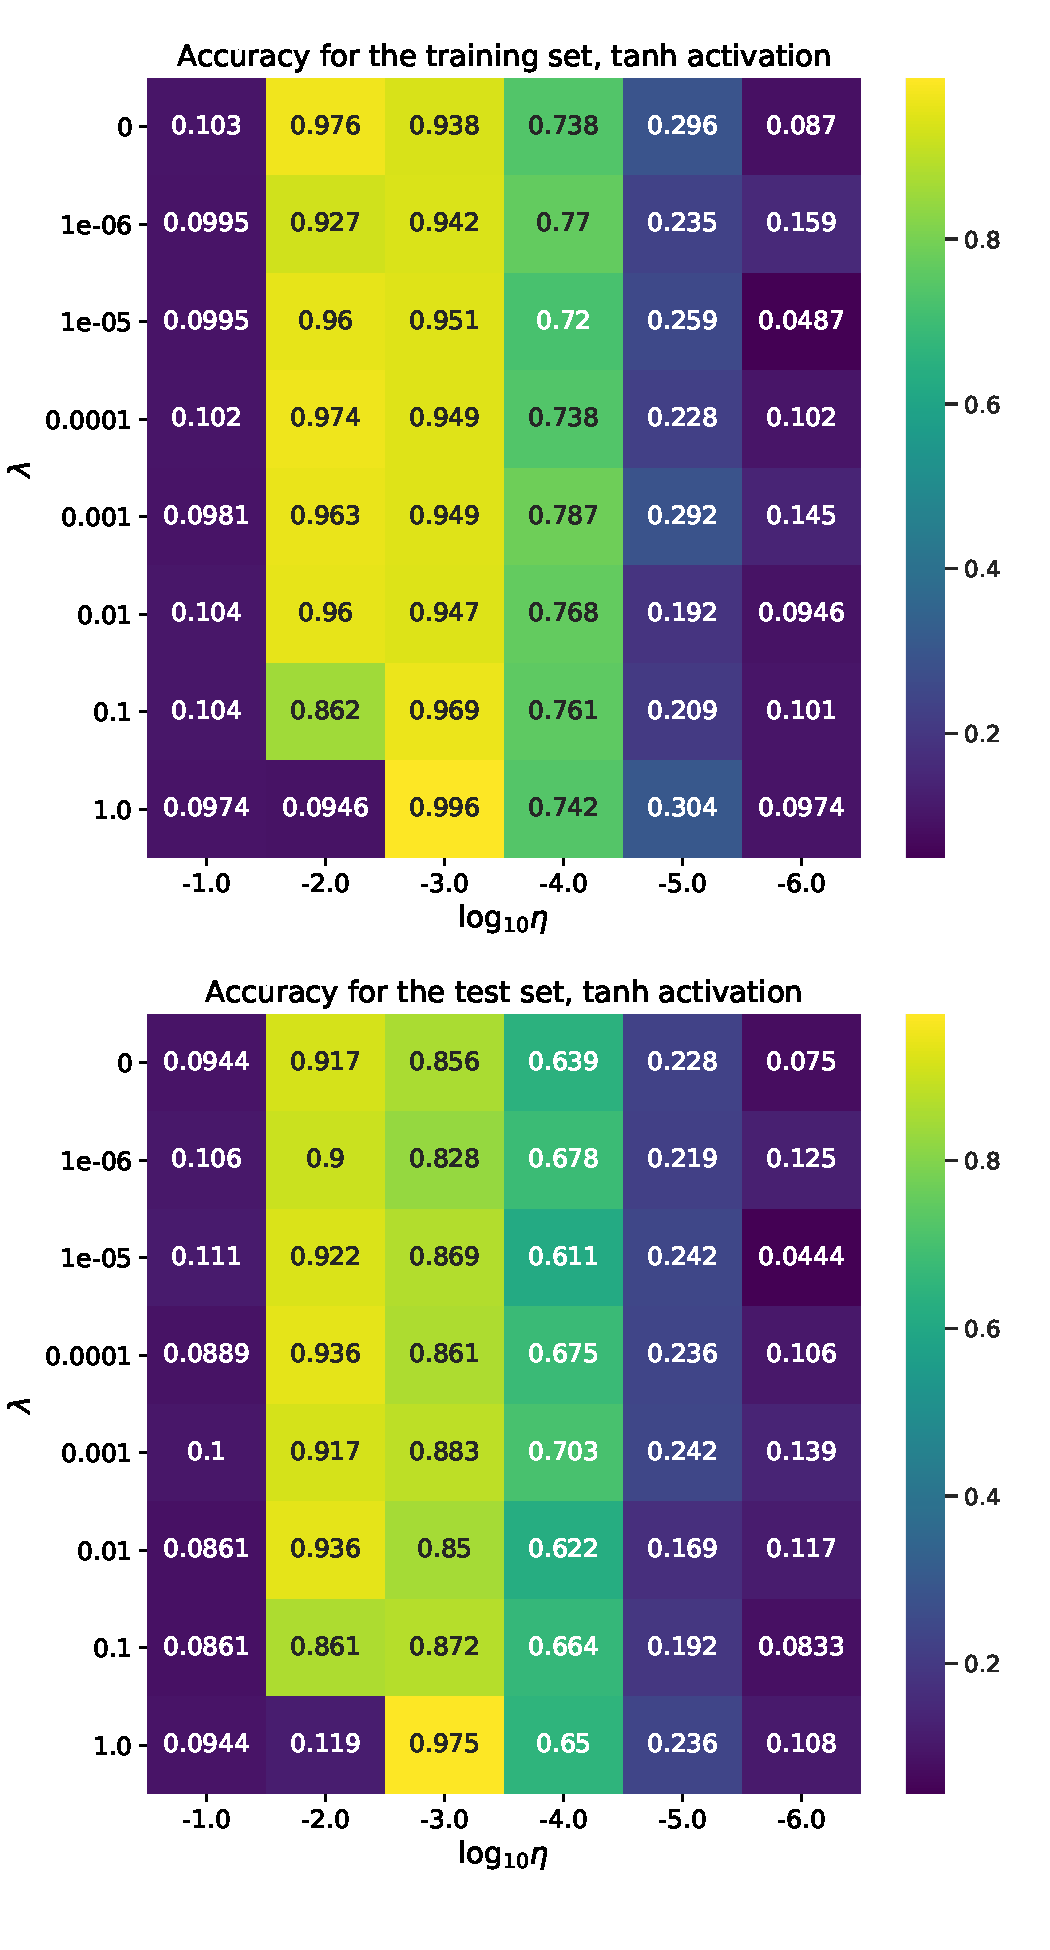
\includegraphics[width=.49\textwidth]{Figures/Class_Ridge_1_layer_tanh.pdf}
    \caption{Grid search for the optimal accuracy for the test and training sets presented as a functions of the learning rate and regularization parameter $\lambda$, 100 epochs, $M=50$. One hidden layer with tanh activation function ($a=0.001$) and 50 neurons is used.}
    \label{fig: grid search class 1 layer tanh}
\end{figure}


Furthermore, we compare our FFNN to the Scikit-Learn and TensorFlow Keras results. The results are shown in Table \ref{tab:Accuracy for FFNN with Keras}. Here we see that our FFNN performs quite well, but the overall best results are achieved with the Scikit-Learn FFNN with SGD. 


\begin{table}[!htb]
\begin{center}
\caption{\scriptsize The accuracy for the test and training sets obtained with $\lambda=0.0$ and $\lambda>0.0$. For all NN 100 epochs, $\eta=0.01$, minibatch size $M=$50 are used. In case of Keras NN $\lambda=0.001$, in other cases $\lambda=0.01$.}
\label{tab:Accuracy for FFNN with Keras}  
\begin{tabular}{lllll}
\cline{2-5}
\noalign{\smallskip}
& \multicolumn{4}{c}{Classification accuracy}\\
\cline{2-5}\noalign{\smallskip}
& \multicolumn{2}{c}{$\lambda = 0$} & \multicolumn{2}{c}{$\lambda > 0$}\\ \cline{2-5}\noalign{\smallskip} 
& Train & Test & Train & Test \\ \hline\noalign{\smallskip}
\multicolumn{1}{l|}{FFNN} & 1.0000 & 0.9333 & 1.0000 & 0.9389\\
\multicolumn{1}{l|}{FFNN SKL (SGD)} & 0.9993 & 0.9694 & 0.9993 & 0.9611\\
\multicolumn{1}{l|}{FFNN SKL (ADAM)} & 0.9680 & 0.9417 & 0.9784 & 0.9611\\
\multicolumn{1}{l|}{FFNN Keras (SGD)} & 0.6374 & 0.6306 & 0.6681 & 0.5972\\
\multicolumn{1}{l|}{FFNN Keras (ADAM)} & 0.6374 & 0.6306 & 0.6681 & 0.5972\\
 \noalign{\smallskip}\hline
\end{tabular}
\end{center}
\end{table}

\subsection{Logistic regression}
\label{subsec:logistic regression results}

Finally, we also study the accuracy of Logistic regression. In Table \ref{tab:Accuracy FFNN and logistic regression} we see how well our LR with SGD and GD performs compared to our FFNN and the Scikit-Learn LR. Here we see that our FFNN with 6 hidden layers performs the best without regularization, whereas the Scikit-Learn LR performs best with regularization. 

\begin{table}[!htb]
\begin{center}
\caption{\scriptsize The accuracy for the test and training sets obtained with $\lambda=0.0$ and 0.01. For the FFNN 100 epochs are used, $\eta=0.01$, minibatch size$=$50. In case of LR+SGD the same settings are used, for LR+GD 10000 iterations and $\eta=0.01$ were used. The Scikit-Learn logistic regression is used with the default settings.}
\label{tab:Accuracy FFNN and logistic regression}  
\begin{tabular}{lllll}
\cline{2-5}
\noalign{\smallskip}
& \multicolumn{4}{c}{Classification accuracy}\\
\cline{2-5}\noalign{\smallskip}
& \multicolumn{2}{c}{$\lambda = 0$} & \multicolumn{2}{c}{$\lambda > 0$} \\ \cline{2-5}\noalign{\smallskip} 
& Train & Test & Train & Test \\ \hline\noalign{\smallskip}
\multicolumn{1}{l|}{FFNN 3 hidden layers} & 1.0000 & 0.9333 & 1.0000 & 0.9389\\
\multicolumn{1}{l|}{FFNN 6 hidden layers} & 1.0000 & 0.9611 & 1.0000 & 0.9639\\
\multicolumn{1}{l|}{LR+SGD} & 0.9903 & 0.9556 & 0.9903 & 0.9556\\
\multicolumn{1}{l|}{LR+GD} & 0.9986 & 0.9583 & 0.9986 & 0.9583\\
\multicolumn{1}{l|}{SKL LR} & 1.0000 & 0.9472 & 1.0000 & 0.9667\\
 \noalign{\smallskip}\hline
\end{tabular}
\end{center}
\end{table}

\section{Discussion of the results}  
\label{sec: Discussion}


\section{Perspectives for further improvements} 
\label{sec: Improvements}

One of the desired improvements which will be implemented in the next project is including the validation set alongside the training and test sets and the early stopping mechanism. It is used for the preliminary assessment of the trained model (NN) performance before making predictions on the test data. An overfitting and underfitting problems for the validation set imply that we must expect similar problems for the test set as well. These issues can be traced and avoided by adjusting the parameters for the better performance on the validation and, correspondingly, test sets. In this project all parameters were chosen to achieve good performance on the test set and both overfitting and underfitting are not as apparent and are not expected to be a great issue for the analysis. However, this situation might change significantly if the NN is applied to a different dataset. In case of this project, the early stopping option might be especially crucial for studies with ReLU and leaky ReLu activation functions of the hidden layers. An uneven distribution of the learning rates and $\lambda$ yielding high scores might become an issue in both regression and classification analysis. An option of creating a validation set will be further implemented in the \textit{data\_processing.py} as the early stopping mechanism will be set as an additional function coupled to the grid search. In addition, further assessment of the scores can be coupled to the k-fold cross-validation, and, therefore, more reliable estimates of the scores as functions of the increasing number of hidden layers, neurons, number of epochs and learning rates can be achieved. In overall, implementation of the early stop while searching for the optimal parameters will save computational time which can be used for performing cross-validation and improvement of reliability of the results.

\section{Conclusions} 
\label{sec: Conclusions}


\section{Appendix A: Link to all programs}
\label{Appendix:A}
\href{https://github.com/tellefs/ML-projects/tree/master/project2}{Link to the project in Github}

\section{Appendix B: Study of different NN architecture types}
\label{Appendix:B}

One additional test to be performed with the FFNN is to study different architectures by selecting different number of neurons in each hidden layer. Here we propose three different architectures shown in Fig.\ref{fig:architectures}. The first type is characterized by an equal distribution of neurons in each, exploiting 5 hidden layers with 150 neurons in total and 30 neurons per layer. The second type has a gradually increasing (by 10) number of neurons in consecutive layers, starting from 10 and ending with 50 neurons. Finally, the third type has a gradually decreasing number of neurons from the first to the last hidden layer. All three types of NN were applied to the regression problem on Franke's data and the classification problem on MNIST data. In the first case, the $R^2$ scores and MSE were estimated for the training and the sets sets, as for the classification of MNIST data these scores were substituted by accuracy. All results obtained are shown in Table \ref{tab:architectures}.

In case of the regression problem it can be seen that the first type of architecture (even distribution of neurons) yields the highest $R^2$ scores of all and, correspondingly, the lowest MSE for both the training and the test sets. The third type of architecture yields slightly smaller, but comparable $R^2$ scores and slightly bigger MSEs. However, the difference between the scores for the first and the third types is in the fourth digit after the decimal and one could safely conclude that both types perform equally well. The second type of architecture results in somewhat worse results. In case of our analysis, the performance seems to improve if a certain number of neurons larger than 10 is used in the first hidden layer. Three tests are not sufficient to make a solid conclusion. However, this study supports the choice of 3 layers with an equal number of neurons in each used in the project for the majority of tests.

In case of classification problem the third type of NN demonstrates the best performance, as the first one yields slightly lower accuracy. Again, the second type performs worse that the first and the third, but the difference is more noticeable than in the regression problem. relatively high classification accuracy for the first type of NN supports the choice of three hidden layers with equal number of neurons applied to the MNIST data.

\begin{figure}[h]
    \centering
    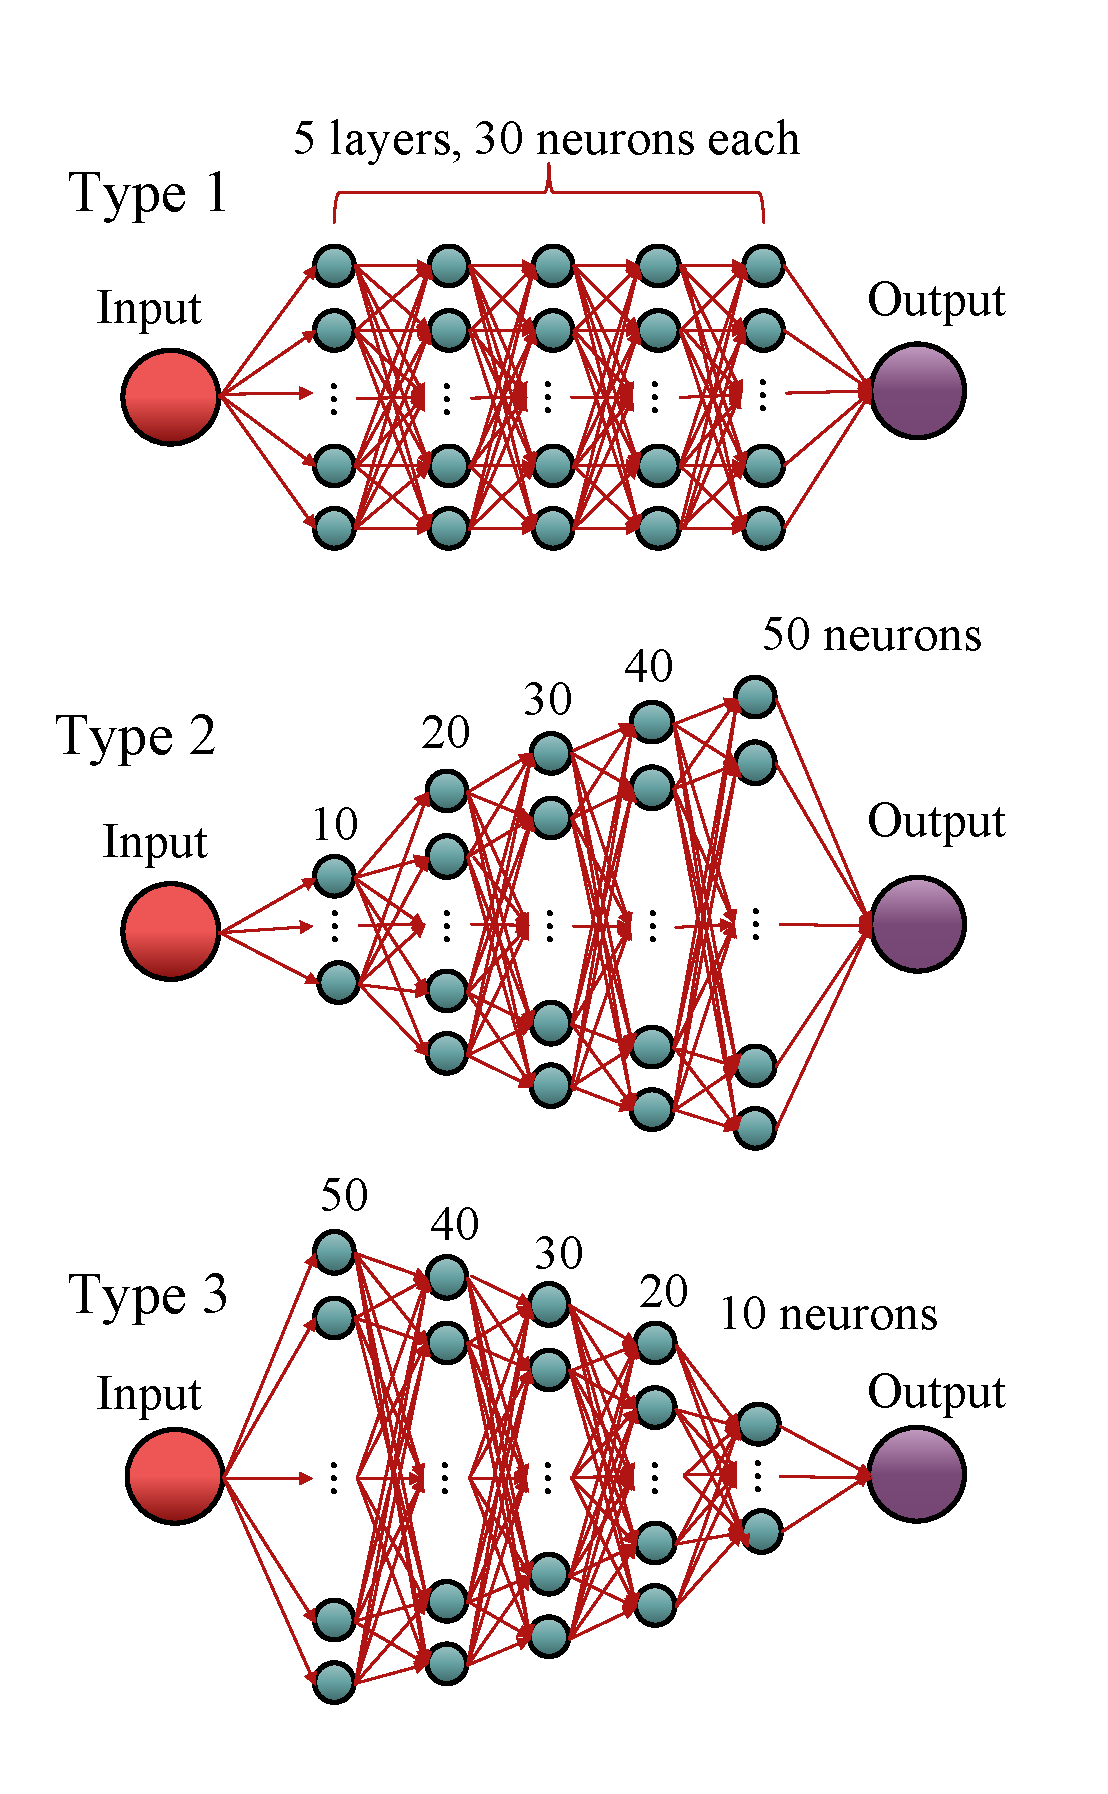
\includegraphics[width=.39\textwidth]{Figures/architectures.pdf}
    \caption{Three different types of NN architecture.}
    \label{fig:architectures}
\end{figure}

\begin{table}[!htb]
\begin{center}
\caption{The MSE, $R^2$ scores and accuracy for the test and training datasets obtained with the FFNN with three different architectures. For the regression problem 1000 epochs, $\lambda=0.0$, $\eta=0.001$ and minibatch size$=$5 were used. In case of classification, 100 epochs, $\eta=0.01$, minibatch size$=$50 were used.}
\label{tab:architectures}  
\begin{tabular}{lllll}
\cline{2-5}
\noalign{\smallskip}
& \multicolumn{4}{c}{Regression}\\
\cline{2-5}\noalign{\smallskip}
& \multicolumn{2}{c}{$R^2$} & \multicolumn{2}{c}{MSE}\\
\cline{2-5}\noalign{\smallskip} & Train &  Test  & Train & Test \\
\hline\noalign{\smallskip}
\multicolumn{1}{l|}{Type 1} & 0.9982 & 0.9941 & 0.0019 & 0.0050 \\
\multicolumn{1}{l|}{Type 2} & 0.9948 & 0.9820 & 0.0053 & 0.0156 \\
\multicolumn{1}{l|}{Type 3} & 0.9979 & 0.9934 & 0.0021 & 0.0056 \\
\hline\noalign{\smallskip}
& \multicolumn{4}{c}{Classification, accuracy}\\
\cline{2-5}\noalign{\smallskip}
& \multicolumn{2}{c}{Train} & \multicolumn{2}{c}{Test}\\
\hline\noalign{\smallskip}
\multicolumn{1}{l|}{Type 1} & \multicolumn{2}{c}{0.9736} & \multicolumn{2}{c}{0.9250} \\
\multicolumn{1}{l|}{Type 2} & \multicolumn{2}{c}{0.9450} & \multicolumn{2}{c}{0.9250}  \\
\multicolumn{1}{l|}{Type 3} & \multicolumn{2}{c}{0.9833} & \multicolumn{2}{c}{0.9417} \\
\hline
\end{tabular}
\end{center}
\end{table}

\section{Appendix C: Additional figures}
\label{Appendix:C}

The following Appendix contains some of the results excluded from the main analysis. Firstly, the results for the training and test MSE presented in form of the grid search for the three layer FFNN are shown in Fig.\ref{fig: NN_Ridge_MSE}. As it was shown for the stochastic gradient descent in Section \ref{sec: Results}, high $R^2$ scores correlate with the low MSE values, and it can be seen that the lowest test and train MSE can be achieved with $\eta=0.01$ and $\lambda=0.001$. The values $\eta=0.001$ and $\lambda=0.001$ chosen for the analysis in the project correspond to the area of low MSE values.

\begin{figure}[!ht]
    \centering
    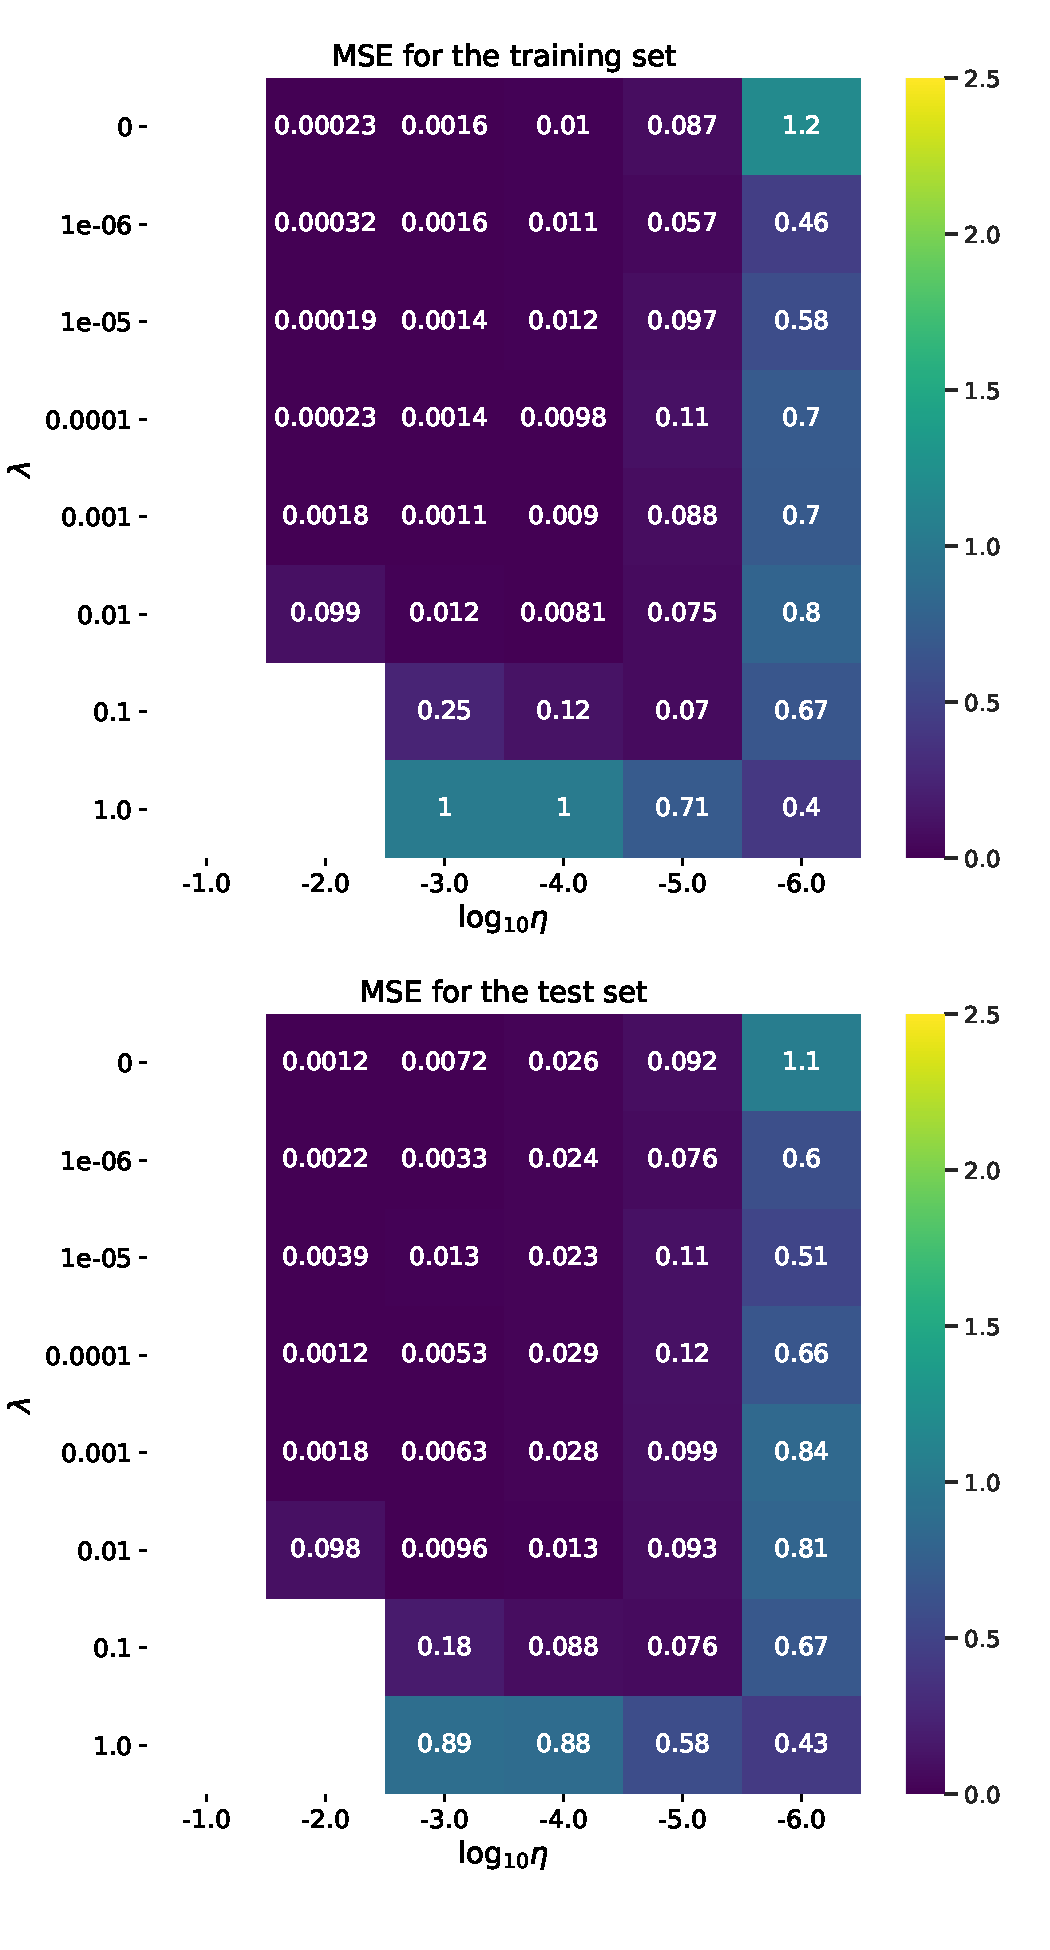
\includegraphics[width=.49\textwidth]{Figures/NN_Ridge_MSE.pdf}
    \caption{Grid search for the optimal $\lambda$ and $\eta$ minimizing the training (upper panel) and test (lower panel) MSE for the three-layer FFNN (50 neurons each), $N_{\mathrm{epochs}}=1000$, $M=5$.}
    \label{fig: NN_Ridge_MSE}
\end{figure}

\begin{figure}[!ht]
    \centering
    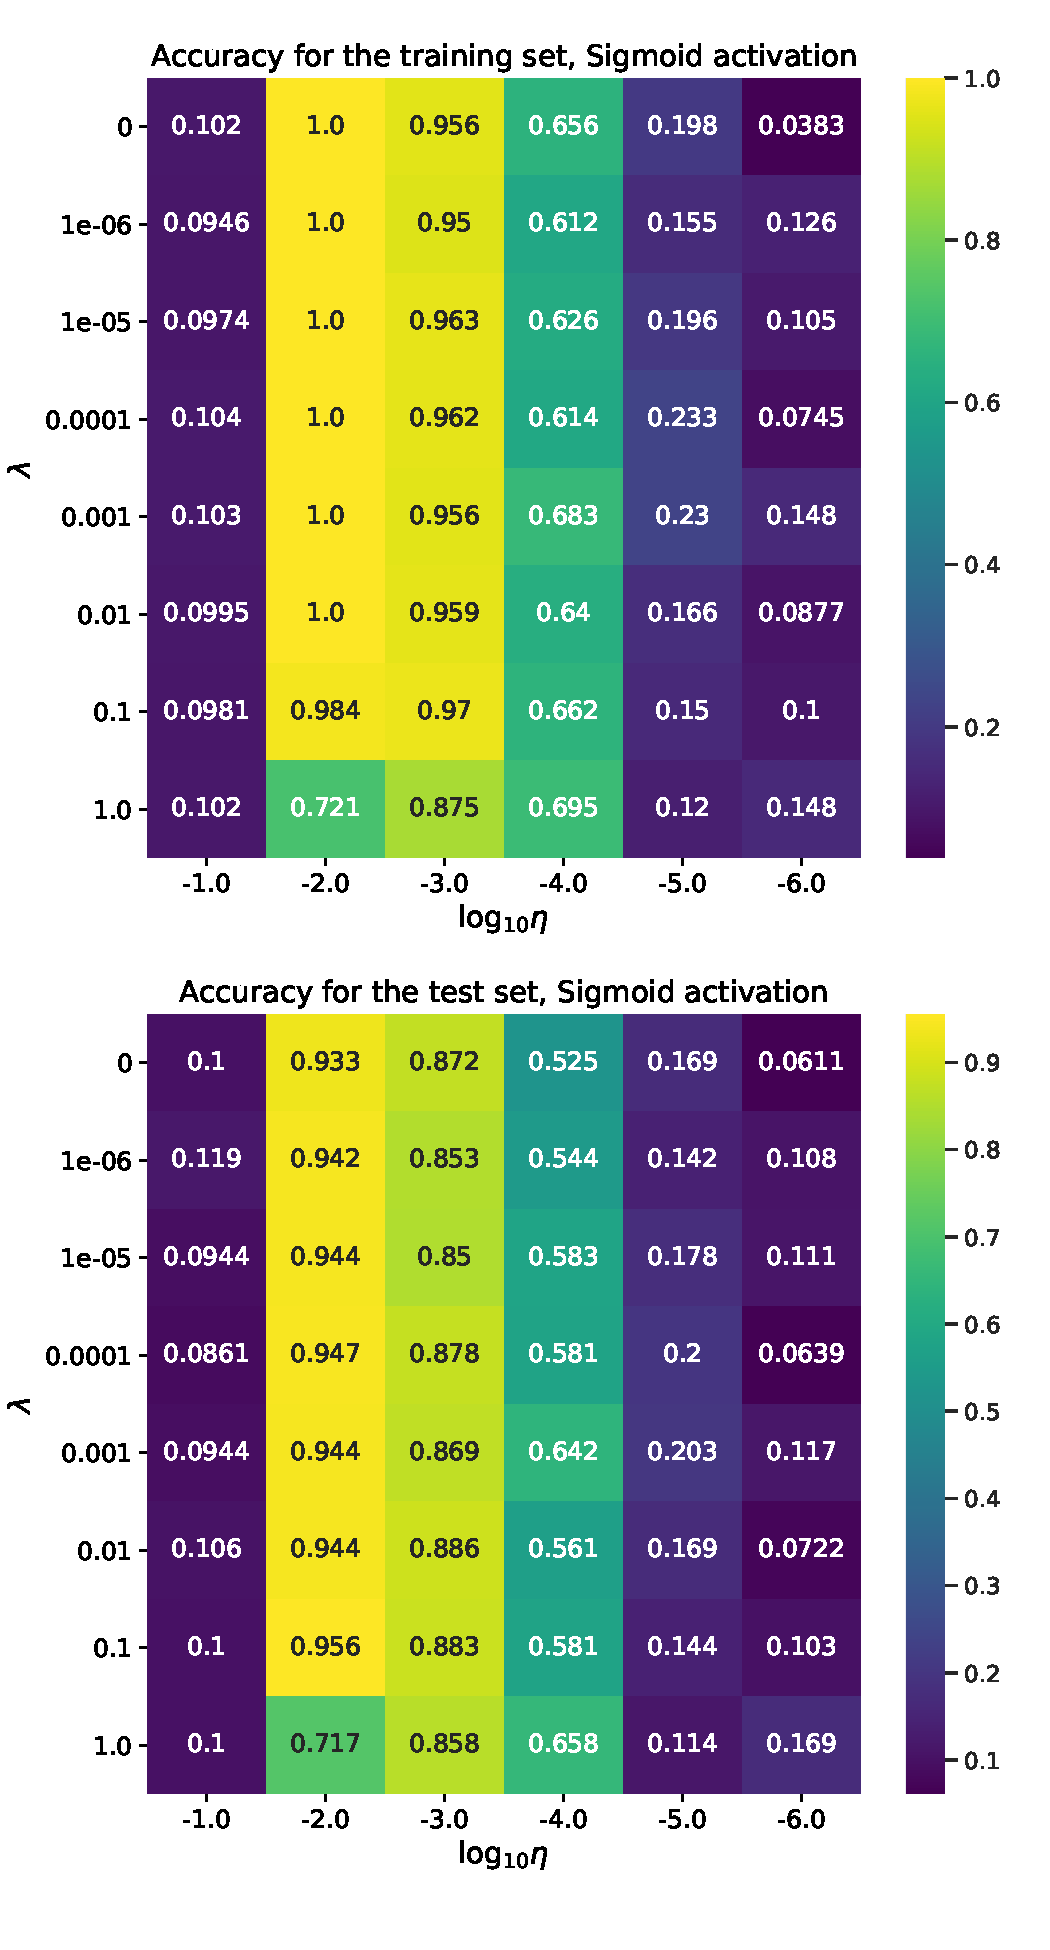
\includegraphics[width=.49\textwidth]{Figures/Class_Ridge.pdf}
    \caption{Grid search for the optimal accuracy for the test and training sets presented as a functions of the learning rate and regularization parameter $\lambda$, 100 epochs, $M=50$. Three hidden layers with 50 neurons are used.}
    \label{fig: grid search class 3 layer}
\end{figure}

Fig.\ref{fig: grid search class 3 layer} presents the grid search of an optimal learning rate value and regularization parameter $\lambda$ for the 3 layer FFNN specified for the classification task. Here, 100 epochs and 50 data points in each minibatch were used. The accuracy obtained for both the test and training sets are especially close to those from Fig.\ref{fig: grid search class 1 layer} obtained for the NN with one layer only. In overall, accuracy for both dataset is slightly higher and it correlates with a slight increase of of accuracy with number of hidden layers observed in Fig.\ref{fig:accuracy vs hidden layers}. The range of the learning rates yielding high scores is quite narrow, $\eta\approx10^{-3}-10^{-2}$. The accuracy degrades fast with the increasing learning rate and relatively slow with the decreasing learning rate. A wide range of $\lambda\approx0-0.1$ seems to yield almost equally high scores for $\eta\approx10^{-3}-10^{-2}$. The highest test accuracy can be achieved with $\eta=0.01$ and $\lambda=0.1$, bit these values do not yield the highest training accuracy. In overall, $\eta=0.01$ and $\lambda=0.01$ chosen for the analysis and comparison of different methods in the project is a reasonable choice providing 100\% training accuracy and relatively high test accuracy. 

\section{Appendix D: study of the ridge case for SGD}
\label{Appendix:D}

By analogy with with the study of the OLS with SGD presented in sec.\ref{sec: Results}, study of the test and training $R^2$ scores and MSE as functions of different parameters was performed for the Ridge case with three different regularization parameters $\lambda=0.1,0.01,0.001$. Firstly, the test and training $R^2$ scores were studied as functions of the learning rate. The results for all three values of $\lambda$ are displayed in Fig.\ref{fig: R2_Ridge_eta}. In all cases, the training score is slightly higher than that for the test set, as expected for the chosen parameters. The test $R^2$ are particularly close to the training scores and are close to the maximum value 1, implying good performance of the model for fitting the Franke's function. A zoomed section of the same graph is presented in Fig.\ref{fig: R2_Ridge_eta_zoom}. It can be seen that the regularization parameter $\lambda=0.001$ gives essentially the same results as in the OLS case. Increased parameter $\lambda=0.01$ still yields the high scores, but the highest of considered parameters, $\lambda=0.1$, leads to a noticeable worsening of the fit quality for the learning rates $\eta\sim 10^{-5}-10^{-3}$. It is important to notice an especially poor performance of the model for particularly small values of $\eta\sim 10^{-6}$. The $R^2$ score for both data sets for all parameters $\lambda$ drops below zero, meaning worse predictions as compared to the baseline model, predicting always the mean value or the target values. Indeed, one should not expect good performance for low values of learning rates and 1000 epochs only. Increasing number of epochs will improve predicting ability of the model, but will simultaneously increase CPU run times considerably.

\begin{figure}[h]
    \centering
    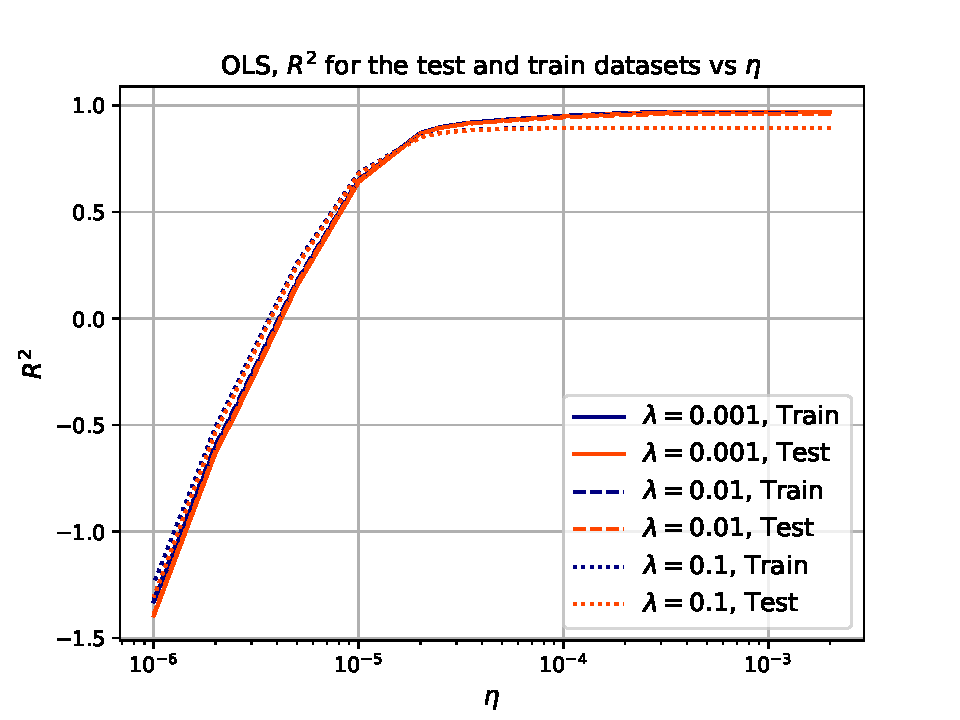
\includegraphics[width=.49\textwidth]{Figures/Ridge_R2_eta.pdf}
    \caption{$R^2$ scores for the test and training datasets obtained with SGD and 5-fold cross-validation with $N_{\mathrm{epochs}}=1000$ and $M=5$ for different learning rates. Ridge case for $\lambda=0.1,0.01,0.001$.}
    \label{fig: R2_Ridge_eta}
\end{figure}

\begin{figure}[h]
    \centering
    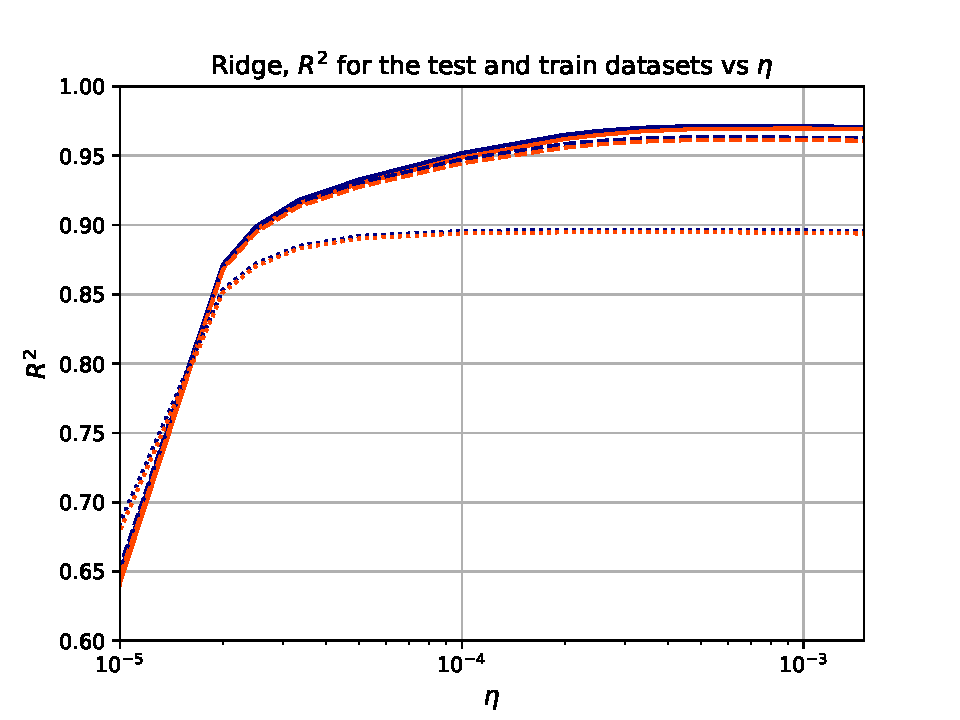
\includegraphics[width=.49\textwidth]{Figures/Ridge_R2_eta_zoom.pdf}
    \caption{Zoomed graph: $R^2$ scores for the test and training datasets obtained with SGD and 5-fold cross-validation with $N_{\mathrm{epochs}}=1000$ and $M=5$ for different learning rates. Ridge case for $\lambda=0.1,0.01,0.001$.}
    \label{fig: R2_Ridge_eta_zoom}
\end{figure}

The MSE for the test and training sets demonstrates an opposite behavior with the increasing learning rate. As the $R^2$ scores demonstrate monotonous increase, the MSE monotonously drops to the minimum value. This fact is reflected in Fig.\ref{fig: MSE_Ridge_eta} for all regularization parameters.

\begin{figure}[h]
    \centering
    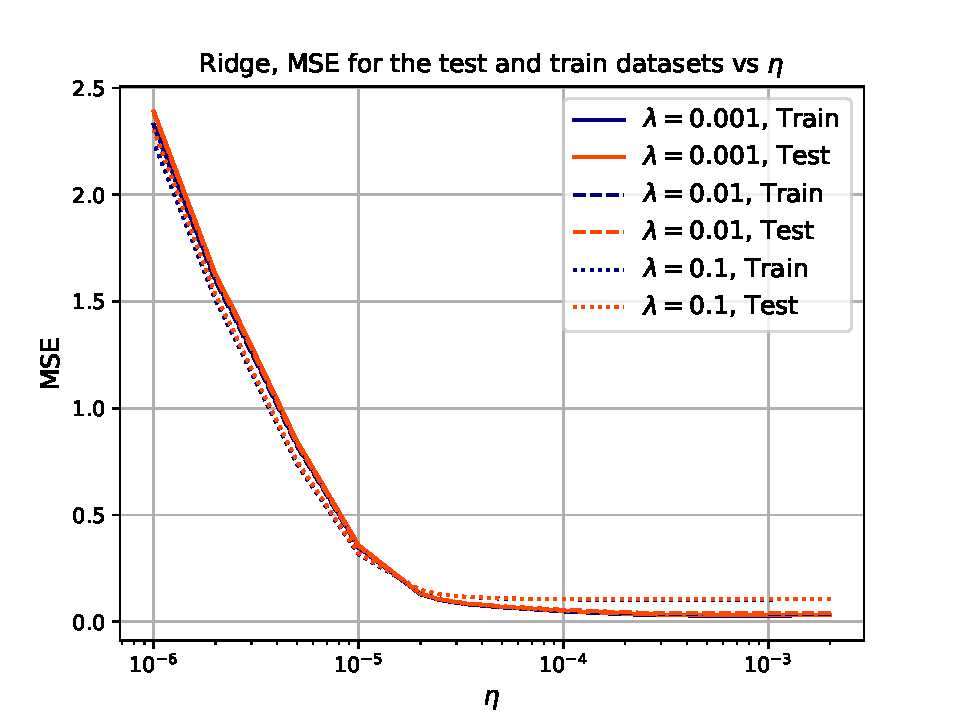
\includegraphics[width=.49\textwidth]{Figures/Ridge_MSE_eta.pdf}
    \caption{MSE for the test and training datasets obtained with SGD and 5-fold cross-validation with $N_{\mathrm{epochs}}=1000$ and $M=5$ for different learning rates. Ridge case for $\lambda=0.1,0.01,0.001$.}
    \label{fig: MSE_Ridge_eta}
\end{figure}

The test and training $R^2$ were also studied as functions of minibatch size $M$. The results for $\lambda=0.1,0.01,0.001$ are shown in Fig.\ref{fig: R2_Ridge_minibatch}. The results for $\lambda=0.001$ are close to those for the OLS case. A noticeable decrease of the scores can be seen for higher values $\lambda=0.1,0.01$. For $\lambda=0.01$ and 0.001 the optimal size of minibatches is clearly seen and corresponds to $M\approx5-10$. For the highest regularization parameter $\lambda=0.1$ the scores remain almost independent (with a slight decrease with $M$) of the minibatch size and no significant improvements can be introduced by tuning $M$.

\begin{figure}[h]
    \centering
    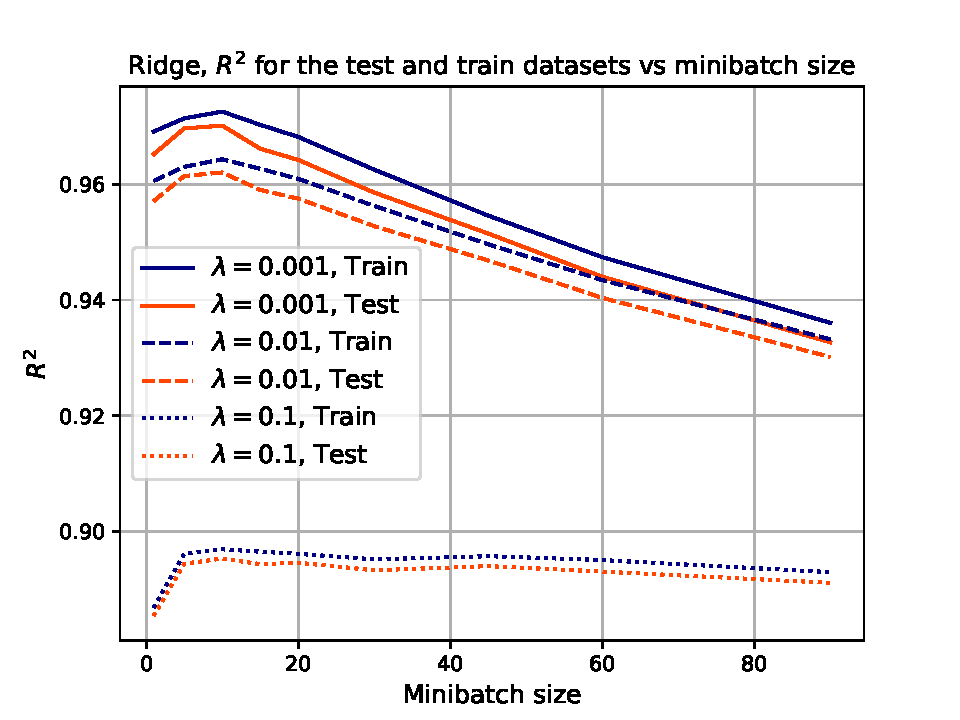
\includegraphics[width=.49\textwidth]{Figures/Ridge_R2_minibatch.pdf}
    \caption{$R^2$ scores for the test and training datasets obtained with SGD and 5-fold cross-validation with $N_{\mathrm{epochs}}=1000$ and $\eta=0.001$ for different sizes of minibatches. Ridge case for $\lambda=0.1,0.01,0.001$.}
    \label{fig: R2_Ridge_minibatch}
\end{figure}

An opposite is observed for the training and test MSE for all regularization parameters and can be seen in Fig.\ref{fig: MSE_Ridge_minibatch}. The MSE reaches its minimum at $M\approx5-10$. For $\lambda=0.1$ the MSE remains on almost the same high level for all studies sizes of minibatches.

\begin{figure}[h]
    \centering
    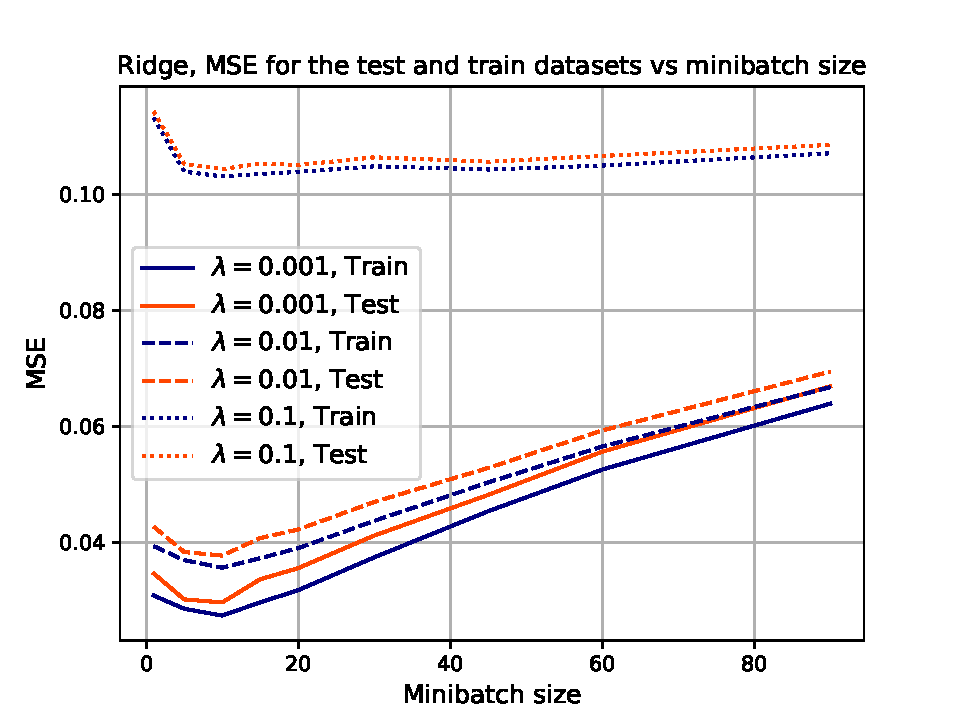
\includegraphics[width=.49\textwidth]{Figures/Ridge_MSE_minibatch.pdf}
    \caption{MSE for the test and training datasets obtained with SGD and 5-fold cross-validation with $N_{\mathrm{epochs}}=1000$ and $\eta=0.001$ for different sizes of minibatches. Ridge case for $\lambda=0.1,0.01,0.001$.}
    \label{fig: MSE_Ridge_minibatch}
\end{figure}

Finally, the $R^2$ scores were studied for different numbers of epochs. The results are displayed in Fig.\ref{fig: R2_Ridge_epochs}. For all regularization parameters the same trend is observed. For  $N_{\mathrm{epochs}}\sim 10-100$ the scores increase fast and reach a plateau at $N_{\mathrm{epochs}}\approx 1000$. The scores for all three regularization parameters remain almost at the constant level with the increasing number of epochs. Collected results for this study demonstrate a local maximum for $N_{\mathrm{epochs}}\approx10^4$ and slight decrease of the scores at $N_{\mathrm{epochs}}\approx10^5$. Practically, further increasing of the number of epochs seems to lead to the overfitting problem similar to that observed for the increasing number of minibatches. The situation with the increasing learning rate is of a different nature: to high values will not allow to reach of approach close enough minimum for the cost function, since the value of $\beta$ will be oscillating around an optimal value with a bigger amplitude as compared to the cases of smaller learning rates. 

\begin{figure}[h]
    \centering
    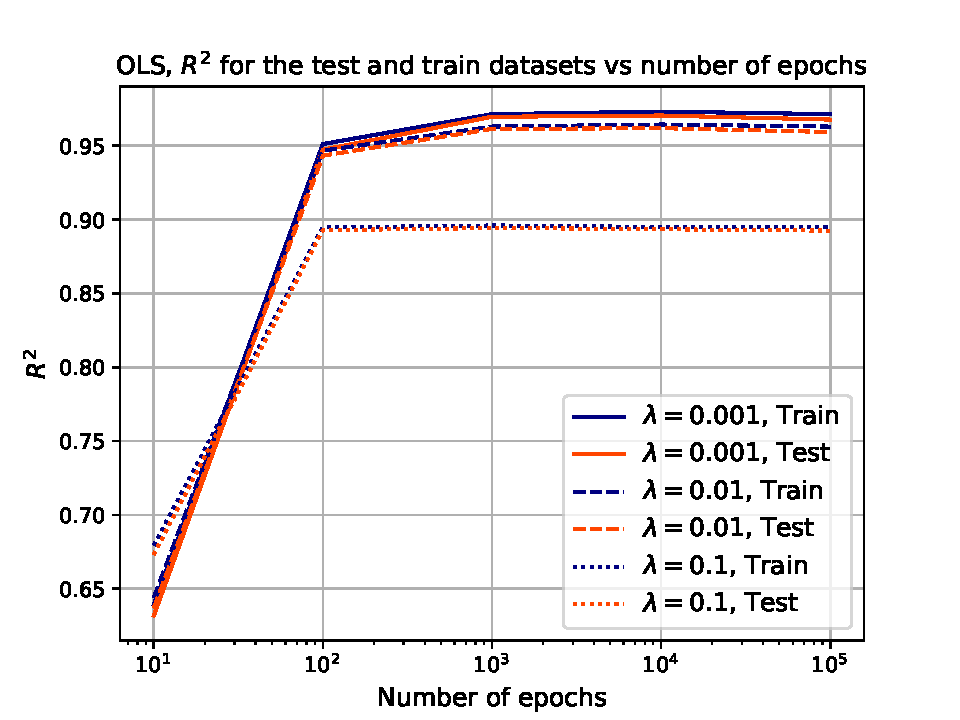
\includegraphics[width=.49\textwidth]{Figures/Ridge_R2_epochs.pdf}
    \caption{$R^2$ scores for the test and training datasets obtained with SGD and 5-fold cross-validation with $M=5$ and $\eta=0.001$ for different numbers of epochs. Ridge case $\lambda=0.1,0.01,0.001$.}
    \label{fig: R2_Ridge_epochs}
\end{figure}

A complementary study of the MSE for the test and training datasets demonstrate a rapid decrease of MSE with the increasing number of epochs. Here, again, the MSE seems to have a certain local minimum at $N_{\mathrm{epochs}}\approx10^4$. 

\begin{figure}[h]
    \centering
    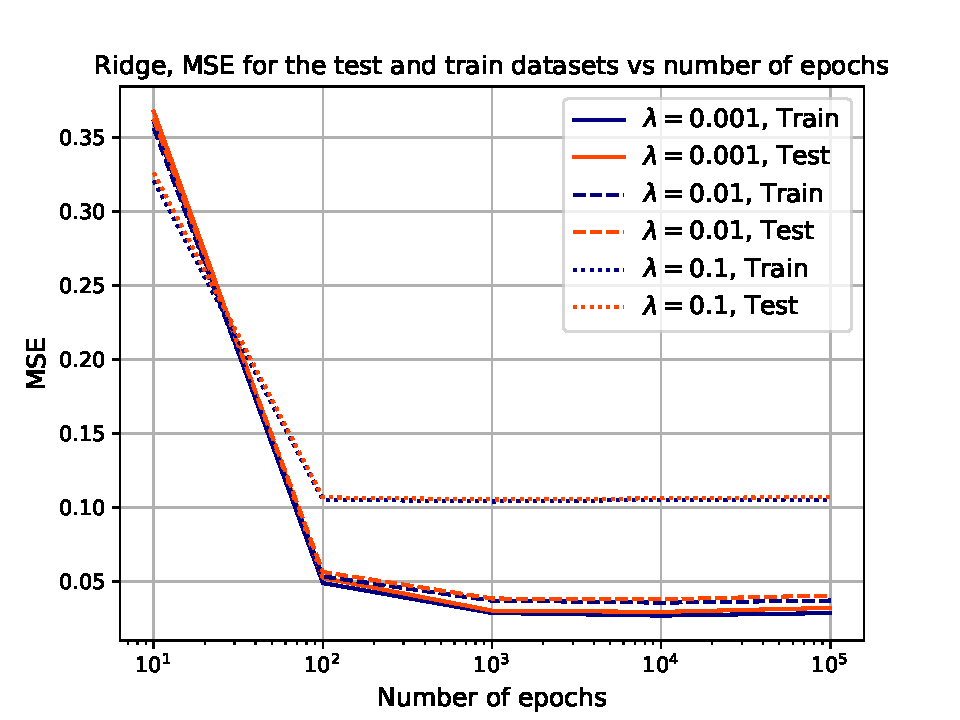
\includegraphics[width=.49\textwidth]{Figures/Ridge_MSE_epochs.pdf}
    \caption{MSE for the test and training datasets obtained with SGD and 5-fold cross-validation with $M=5$ and $\eta=0.001$ for different numbers of epochs. OLS case $\lambda=0.1,0.01,0.001$.}
    \label{fig: MSE_Ridge_epochs}
\end{figure}

\newpage
%////////////////////////////////////////////////////////////////
\begin{thebibliography}

\bibitem{proj1}
L. G. Pedersen and M. L. Markova, "Analysis of the data with the linear regression methods with application of resampling techniques", October 9, 2020. URL: \url{https://github.com/linegpe/FYS-STK4155/tree/master/Project1}, accessed November 2, 2020.

\bibitem{proj1_2}
J. E. Vevik and T. Storebakken, "Regression analysis and resampling techniques", October 7, 2020. URL: \url{https://github.com/tellefs/ML-projects/tree/master/project1}, accessed November 2, 2020.

\bibitem{MNIST}
Y. LeCun, C. Cortes and C. J. C. Burges, "The MNIST database of handwritten digits". URL: \url{http://yann.lecun.com/exdb/mnist/}, last accessed November 2, 2020.

\bibitem{Morten}
H.J. Morten // Applied Data Analysis and Machine Learning, FYS-STK4155 - lecture notes fall 2020.

\bibitem{skl}
Scikit-learn user guide and documentation, Release 0.23.2: URL: \url{https://scikit-learn.org/stable/_downloads/scikit-learn-docs.pdf}, last accessed November 4, 2020.

\bibitem{numpy}
NumPy documentation: \url{https://numpy.org/doc/}, last accessed November 4, 2020.

\bibitem{keras}
Keras documentation:
\url{https://faroit.com/keras-docs/1.2.0/}, last accessed November 4, 2020.

\end{thebibliography} 


\end{document}



%-------------------------SAMPLES OF TABLES AND FIGURES ---------------------
